\documentclass[12pt,a4paper]{report}
\pdfminorversion=7
\usepackage[utf8]{inputenc}
\usepackage[T1]{fontenc}
\usepackage[italian]{babel}
\usepackage[margin=2.5cm]{geometry}
\usepackage{amsmath}
\usepackage{graphicx}
\usepackage[normalem]{ulem}
\usepackage{float}
\usepackage{pdflscape}
\usepackage{array,booktabs,longtable,xltabular}
\usepackage{enumitem}
\usepackage[table]{xcolor}
\usepackage{listings}
\usepackage{hyperref}
\hypersetup{hidelinks,pdftitle={DriveHub -- Relazione di Ingegneria del Software},pdfauthor={Federico D'Amodio, Matteo Orlandi}}
\graphicspath{{images/}}
\setlist{itemsep=2pt,topsep=4pt}
\renewcommand{\arraystretch}{1.17}
\emergencystretch=2em
\setcounter{tocdepth}{2}
\DeclareRobustCommand{\code}[1]{\nolinkurl{#1}}
\lstset{basicstyle=\ttfamily\small,breaklines=true,frame=single,columns=fullflexible,showstringspaces=false,
  keywordstyle=\color{blue!60!black},commentstyle=\color{green!40!black},captionpos=b}
\newcommand{\dhfigure}[4]{%
  \begin{figure}[htbp]\centering
  \includegraphics[width=#1\linewidth,height=.67\textheight,keepaspectratio]{#2}
  \caption{#3}\label{#4}\end{figure}}

\begin{document}
\hypersetup{pageanchor=false}
\begin{titlepage}
  \centering
  {\Large\textsc{Università degli Studi di Firenze}\par}
  {\large Scuola di Ingegneria\par}
  {\large Corso di Laurea in Ingegneria Informatica\par}
  \vspace{2cm}
  \rule{\linewidth}{.5pt}\par\vspace{.8cm}
  {\Huge\bfseries\color{blue!55!black} DriveHub\par}\vspace{.35cm}
  {\Large\itshape Sistema informativo per la vendita e il noleggio di veicoli\par}
  \vspace{.8cm}\rule{\linewidth}{.5pt}\par
  \vspace{1.7cm}
  \begin{minipage}[t]{.48\linewidth}\raggedright
    \textbf{Candidati:}\\[.3cm]
    Federico D'Amodio\\
    Matteo Orlandi
  \end{minipage}\hfill
  \begin{minipage}[t]{.48\linewidth}\raggedleft
    \textbf{Corso:}\\
    Ingegneria del Software\\[.35cm]
    \textbf{Docente:}\\
    Prof. Enrico Vicario
  \end{minipage}
  \vfill
  {\large Anno Accademico 2025/2026\par}
\end{titlepage}
\hypersetup{pageanchor=true}
\pagenumbering{roman}\tableofcontents\clearpage\pagenumbering{arabic}
\chapter{Introduzione}\label{ch:introduzione}

\section{Descrizione}
\textbf{DriveHub} è un'applicazione desktop per le attività essenziali di un concessionario: presentare i veicoli disponibili, organizzare test drive e noleggi, gestire le richieste di acquisto e valutare le auto proposte dai clienti. Un unico catalogo collega queste operazioni allo stato di ciascun veicolo, così che le scelte degli utenti si riflettano sulla sua disponibilità.

Il sistema prevede tre figure operative:
\begin{itemize}
  \item \textbf{Cliente (\code{CLIENT}):} si registra, consulta il catalogo, prenota un test drive o un noleggio, versa l'acconto per richiedere un acquisto e propone al concessionario un proprio veicolo. Può consultare le proprie operazioni e usare un conto dimostrativo per i movimenti previsti dall'applicazione.
  \item \textbf{Venditore (\code{SALESMAN}):} esamina i veicoli proposti dai clienti e decide se accettarli o rifiutarli; autorizza il completamento delle richieste di acquisto e può cambiare la destinazione di un veicolo tra vendita e noleggio. Nella propria area consulta anche richieste, noleggi e test drive.
  \item \textbf{Manager (\code{MANAGER}):} cura il catalogo inserendo marche, modelli e veicoli, applica sconti a modelli o singole auto e consulta le vendite registrate.
\end{itemize}

Le tre aree condividono le informazioni sul veicolo, ma espongono operazioni diverse in base al ruolo. Nel codice il cliente è identificato da \code{CLIENT}; la denominazione \emph{Customer} compare anche nei materiali di progetto.

\section{Stack tecnologico}
\begin{itemize}
  \item \textbf{Linguaggio e interfaccia:} Java 21 e JavaFX 21.0.2. I layout sono definiti in FXML, lo stile in CSS e le azioni delle schermate nei controller.
  \item \textbf{Organizzazione del codice:} i package \code{presentation}, \code{business}, \code{domain} e \code{dao} separano interfaccia, casi d'uso, regole del dominio e accesso ai dati. Le interfacce DAO sono distinte dalle implementazioni JDBC.
  \item \textbf{Persistenza:} PostgreSQL tramite driver JDBC. All'avvio, se la connessione non riesce, l'applicazione usa un database H2 in memoria in modalità compatibile con PostgreSQL, inizializzato con dati dimostrativi.
  \item \textbf{Sicurezza:} le password sono salvate come hash derivati con PBKDF2, anziché in chiaro.
  \item \textbf{Build e verifica:} Maven gestisce dipendenze e compilazione; JUnit 5 e Mockito supportano i test, JaCoCo la misurazione della copertura.
\end{itemize}

\section{Semplificazioni adottate}\label{sec:semplificazioni}
Per mantenere il progetto realizzabile e dimostrabile, alcuni processi del concessionario sono rappresentati in forma ridotta:
\begin{itemize}
  \item \textbf{Pagamenti interni:} acconti, saldi, noleggi e rimborsi modificano il saldo di un \code{BankAccount} locale. Non sono integrati banche o circuiti di pagamento e i movimenti non costituiscono transazioni finanziarie reali.
  \item \textbf{Account dello staff:} la registrazione consente di scegliere anche i ruoli Venditore e Manager. È una scelta del prototipo; l'attribuzione di questi ruoli in un sistema operativo richiederebbe un controllo amministrativo.
  \item \textbf{Modalità dimostrativa:} H2 permette di avviare l'applicazione senza un server PostgreSQL, ma i dati in memoria non sopravvivono alla chiusura. Questa modalità serve a provare i flussi principali.
  \item \textbf{Processi aziendali:} il sistema registra le operazioni sul veicolo senza modellare sedi, fornitori, officina, consegna fisica, contratti, fatturazione o assistenza successiva alla vendita.
\end{itemize}

La documentazione in \code{docs/} conserva anche requisiti e risultati di una baseline precedente: fra questi, ordini di stock, un gateway di pagamento con stati propri e prove PostgreSQL/GUI più estese. I capitoli 2--4 descrivono il checkout presente in \code{src/} e in \code{src/main/resources/db/migration/init.sql}; quando richiamano un requisito storico non realizzato, ne dichiarano esplicitamente il limite. I risultati dei test sono attribuiti soltanto alla baseline su cui sono stati eseguiti.

Il progetto ha impiegato un assistente di intelligenza artificiale per analisi comparativa, revisione di testo, diagrammi, codice e test; il processo e le verifiche dichiarate dagli autori sono registrati in \code{docs/USO_AI.md}. La presente revisione ha confrontato i file locali e rieseguito la suite standard. I capitoli successivi presentano requisiti, progettazione, implementazione e verifiche del sistema.

\chapter{Analisi dei requisiti e progettazione}\label{ch:progettazione}

\section{Diagramma dei casi d'uso}\label{sec:casi-uso}
Il diagramma mostra le funzioni offerte ai tre ruoli di DriveHub. L'attore generale \emph{User} raccoglie registrazione e accesso; \emph{Customer}, \emph{Salesman} e \emph{Manager} ereditano queste possibilità e accedono alle operazioni delle rispettive aree. Il Customer consulta il catalogo e avvia le operazioni commerciali; il Salesman valuta le proposte e segue le pratiche; il Manager mantiene catalogo e sconti e consulta le vendite. I sei casi d'uso dettagliati sotto comprendono quattro operazioni del Customer, l'autorizzazione di un acquisto da parte del Salesman e la gestione di uno sconto da parte del Manager.

\begin{figure}[H]\centering
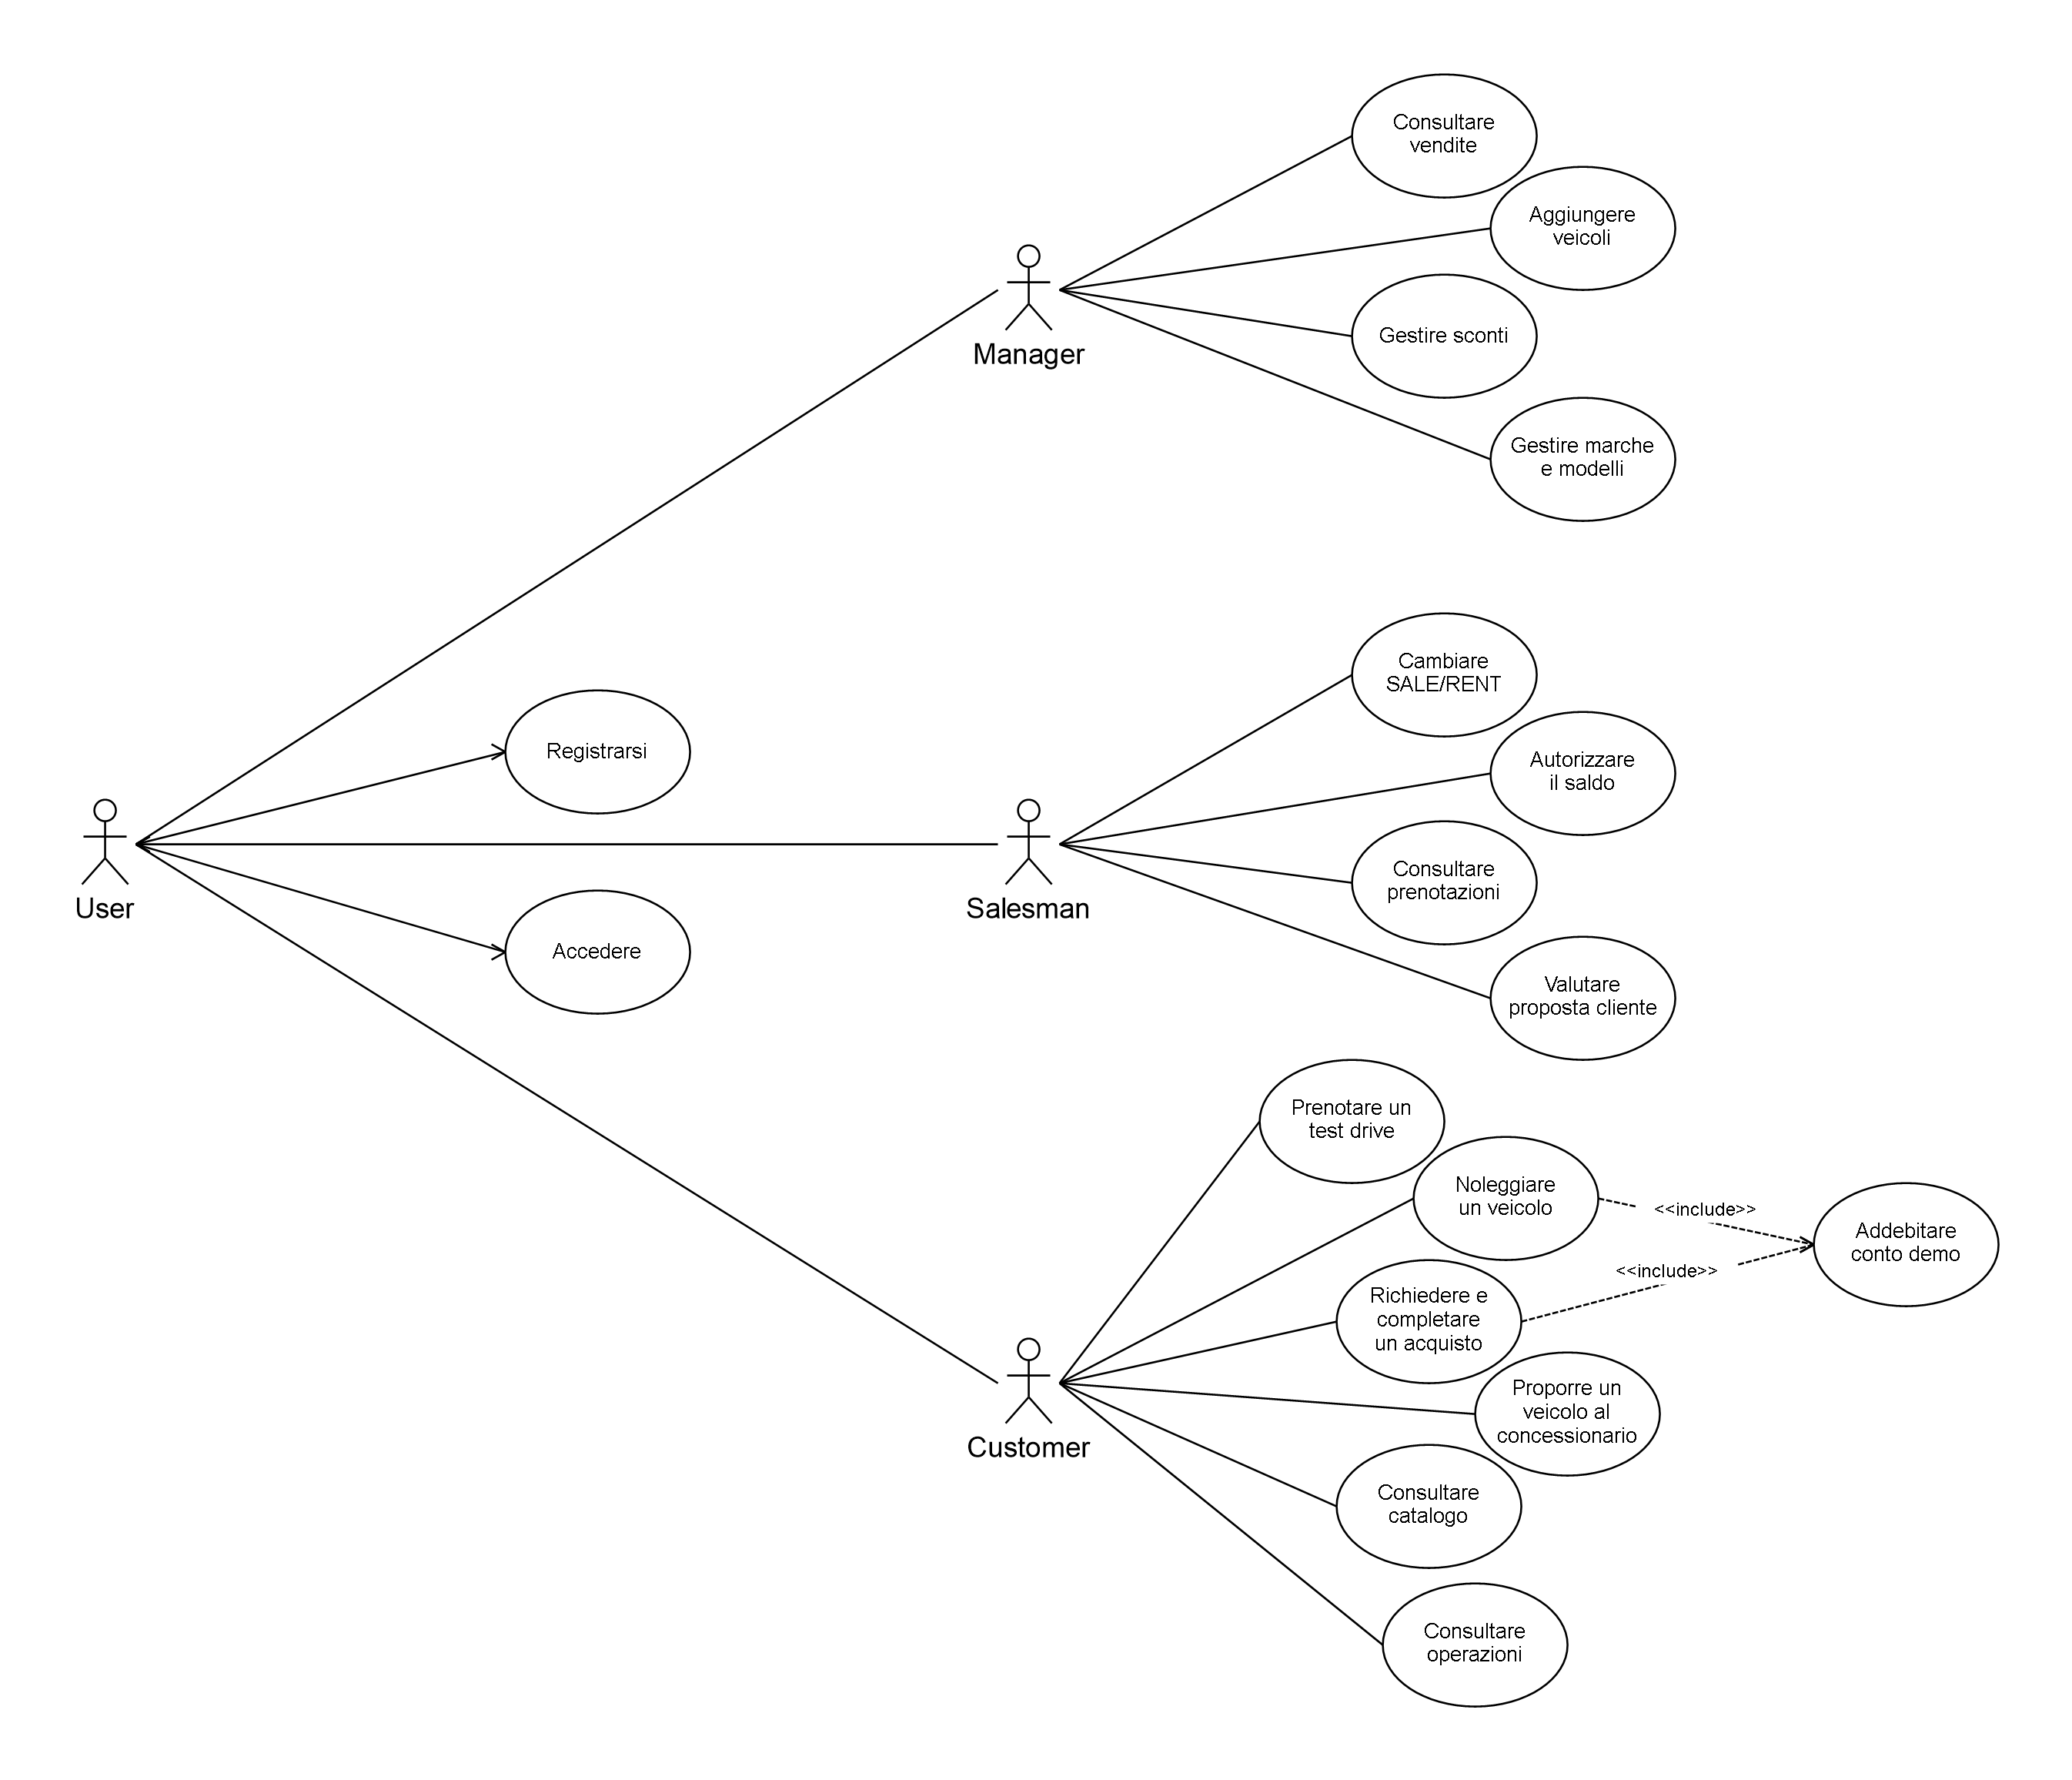
\includegraphics[width=\linewidth,height=.42\textheight,keepaspectratio]{users-swe-current.png}
\caption{Casi d'uso di DriveHub nel codice corrente. Diagramma sorgente: \texttt{docs/Users\ SWE.drawio}.}\label{fig:uc-correnti}
\end{figure}
\clearpage

\section{Template dei casi principali}
Ogni caso d'uso specifica nome, livello, descrizione, pre-condizioni, post-condizioni, attori, test e flussi. Il flusso principale è numerato a partire da 1 in ciascun template. Le alternative sono identificate da A1, A2 e così via, con il rimando al passo principale da cui si diramano. I riferimenti ai test distinguono i comportamenti coperti dalle alternative prive di una prova specifica. Le anomalie implementative sono richiamate separatamente dai flussi quando necessario.
\begingroup\renewcommand{\arraystretch}{1.4}
\subsection{Prenotare un test drive}\label{sec:uc-test-drive}
\begin{xltabular}{\textwidth}{| >{\bfseries}p{.22\textwidth} | >{\raggedright\arraybackslash}X |}
\caption{Caso d'uso: Prenotare un test drive}\label{tab:uc-test-drive}\\
\hline
\rowcolor{gray!15} Campo & \textbf{Contenuto}\\\hline
\endfirsthead
\multicolumn{2}{c}{{\tablename\ \thetable{} -- Continua dalla pagina precedente}}\\
\hline
\rowcolor{gray!15} Campo & \textbf{Contenuto}\\\hline
\endhead
\hline
\multicolumn{2}{r}{\textit{Continua nella pagina successiva...}}\\
\endfoot
\endlastfoot
Nome & Prenotare un test drive\\\hline
Livello & Obiettivo Utente\\\hline
Descrizione & Il Customer prenota una prova di guida di un'ora per un veicolo disponibile nel catalogo.\\\hline
Pre-condizioni & Il Customer ha effettuato l'accesso; il veicolo esiste ed è in stato \code{SALE} o \code{RENT}; la data e la fascia oraria scelte non sono passate.\\\hline
Post-condizioni & Una prenotazione di test drive è registrata per il Customer, il veicolo e lo slot selezionato.\\\hline
Attori & Customer\\\hline
Test & \code{UserGoalsFunctionalTest.bookTestDrive} esercita il percorso principale su H2; \code{RentalWorkflowTest} verifica le regole dell'entità. Non è presente una prova funzionale specifica per ciascuna alternativa o per richieste concorrenti.\\\hline
Flusso Principale &
\begin{enumerate}[label=\arabic*.,start=1,leftmargin=*,nosep]
  \item Il Customer seleziona un veicolo dal catalogo e apre la scheda dei test drive.
  \item Sceglie una data e uno degli orari proposti, dalle 09:00 alle 16:00.
  \item Il sistema verifica che il veicolo sia idoneo, che il Customer abbia meno di tre test drive futuri e che il veicolo non sia noleggiato nella data scelta.
  \item Il sistema verifica che lo slot di un'ora non sia già occupato per quel veicolo.
  \item Il sistema salva la prenotazione e ne comunica l'esito al Customer.
\end{enumerate}\\\hline
Flussi Alternativi &
\textbf{A1 (passo 2). Data o orario non validi:} se lo slot è nel passato o fuori dalla fascia consentita, il sistema rifiuta la prenotazione.\newline\newline
\textbf{A2 (passo 3). Veicolo non idoneo o limite raggiunto:} un veicolo non in vendita né a noleggio, oppure tre test drive futuri già registrati, impedisce il salvataggio.\newline\newline
\textbf{A3 (passi 3--4). Veicolo indisponibile:} un noleggio nel giorno scelto o un altro test drive nello stesso slot produce un conflitto.\newline\newline
\textbf{A4 (passo 4). Richieste concorrenti:} il controllo dello slot precede l'inserimento; il database non impone un vincolo univoco sullo slot, quindi due richieste simultanee potrebbero entrambe riuscire. Inoltre il servizio riconduce i minuti forniti all'inizio dell'ora: un input diretto come 10:30 è trattato come 10:00.\\\hline
\end{xltabular}

\endgroup
\begingroup\renewcommand{\arraystretch}{1.4}
\subsection{Noleggiare un veicolo}\label{sec:uc-noleggio}
\begin{xltabular}{\textwidth}{| >{\bfseries}p{.22\textwidth} | >{\raggedright\arraybackslash}X |}
\caption{Caso d'uso: Noleggiare un veicolo}\label{tab:uc-noleggio}\\
\hline
\rowcolor{gray!15} Campo & \textbf{Contenuto}\\\hline
\endfirsthead
\multicolumn{2}{c}{{\tablename\ \thetable{} -- Continua dalla pagina precedente}}\\
\hline
\rowcolor{gray!15} Campo & \textbf{Contenuto}\\\hline
\endhead
\hline
\multicolumn{2}{r}{\textit{Continua nella pagina successiva...}}\\
\endfoot
\endlastfoot
Nome & Noleggiare un veicolo\\\hline
Livello & Obiettivo Utente\\\hline
Descrizione & Il Customer prenota un veicolo per un intervallo di giorni e paga anticipatamente l'intero importo con il conto dimostrativo.\\\hline
Pre-condizioni & Il Customer ha effettuato l'accesso; il veicolo esiste ed è in stato \code{RENT}; la data iniziale non è passata e la data finale non precede quella iniziale.\\\hline
Post-condizioni & Il noleggio è registrato, l'importo è sottratto dal saldo del Customer e i test drive sul veicolo nei giorni prenotati sono cancellati. Le scritture nel database avvengono nella stessa transazione.\\\hline
Attori & Customer\\\hline
Test & \code{RentalServiceTest.bookRentalDebitsAccount} verifica il servizio con DAO simulati; \code{CheckoutFunctionalTest.rentalBookingWorkflow} verifica il percorso principale su H2. Le alternative di conflitto e la concorrenza non hanno un test funzionale dedicato nella suite corrente.\\\hline
Flusso Principale &
\begin{enumerate}[label=\arabic*.,start=1,leftmargin=*,nosep]
  \item Il Customer seleziona un veicolo disponibile per il noleggio e indica il primo e l'ultimo giorno.
  \item Il sistema mostra un preventivo. Nel conteggio sono inclusi sia il giorno iniziale sia quello finale.
  \item Il Customer conferma la prenotazione.
  \item Il sistema verifica che non vi siano noleggi sovrapposti e calcola l'importo: tariffa giornaliera pari allo 0,1\% del prezzo del veicolo, con un fattore 0,95 applicato per ogni giorno aggiuntivo.
  \item Il sistema addebita l'intero importo sul conto dimostrativo e registra il noleggio.
  \item Il sistema cancella gli eventuali test drive sul veicolo nei giorni prenotati e conferma l'operazione.
\end{enumerate}\\\hline
Flussi Alternativi &
\textbf{A1 (passo 1). Veicolo o date non validi:} il sistema rifiuta la richiesta senza registrare il noleggio.\newline\newline
\textbf{A2 (passo 4). Periodo occupato:} se esiste un noleggio che condivide almeno un giorno, l'operazione è rifiutata.\newline\newline
\textbf{A3 (passo 4). Richieste concorrenti:} la verifica delle sovrapposizioni non è protetta da un vincolo di esclusione nel database; due richieste simultanee potrebbero entrambe riuscire.\newline\newline
\textbf{A4 (passo 5). Saldo insufficiente:} l'addebito fallisce; la transazione annulla anche le altre scritture.\\\hline
\end{xltabular}

\endgroup
\clearpage
\begingroup\renewcommand{\arraystretch}{1.4}
\subsection{Richiedere e completare un acquisto}\label{sec:uc-acquisto}
\begin{xltabular}{\textwidth}{| >{\bfseries}p{.22\textwidth} | >{\raggedright\arraybackslash}X |}
\caption{Caso d'uso: Richiedere e completare un acquisto}\label{tab:uc-acquisto}\\
\hline
\rowcolor{gray!15} Campo & \textbf{Contenuto}\\\hline
\endfirsthead
\multicolumn{2}{c}{{\tablename\ \thetable{} -- Continua dalla pagina precedente}}\\
\hline
\rowcolor{gray!15} Campo & \textbf{Contenuto}\\\hline
\endhead
\hline
\multicolumn{2}{r}{\textit{Continua nella pagina successiva...}}\\
\endfoot
\endlastfoot
Nome & Richiedere e completare un acquisto\\\hline
Livello & Obiettivo Utente\\\hline
Descrizione & Il Customer riserva un veicolo in vendita versando un acconto; dopo l'autorizzazione del Salesman, paga il saldo e conclude l'acquisto. Le azioni possono avvenire in sessioni diverse.\\\hline
Pre-condizioni & Customer e Salesman hanno effettuato l'accesso alle rispettive aree; il veicolo esiste ed è in stato \code{SALE}; il Customer dispone dell'importo necessario per l'acconto.\\\hline
Post-condizioni & Dopo l'acconto il veicolo è \code{BLOCKED} e la richiesta è registrata. Dopo il saldo il veicolo è \code{SOLD}, la richiesta è eliminata, la vendita è registrata e gli eventuali test drive futuri sono cancellati. Ciascuna fase ha una propria transazione.\\\hline
Attori & Customer (primario), Salesman\\\hline
Schermate & Passi 1--2: catalogo (figura~\ref{fig:ui-catalogo}); passo 3: richieste Salesman (figura~\ref{fig:ui-salesman-richieste}); passi 4--6: acquisti del Customer (figura~\ref{fig:ui-acquisti}) e conto (figura~\ref{fig:ui-conto}).\\\hline
Test & \code{CheckoutFunctionalTest.completePurchaseWorkflow} verifica il percorso principale su H2; \code{cancelPurchaseWorkflowWithPenalty} verifica l'annullamento. \code{SalesServiceTest} verifica avvio e penale con mock. Autorizzazione assente, scadenza e variazione del prezzo non sono coperti da una prova funzionale dedicata.\\\hline
Flusso Principale &
\begin{enumerate}[leftmargin=*,nosep]
  \item Il Customer seleziona un veicolo in vendita; l'interfaccia calcola l'acconto, pari al 20\% del prezzo visualizzato. Il saldo finale usa invece \code{Vehicle.price}, che può differire dal prezzo visualizzato in presenza di sconti.
  \item Il Customer conferma: il sistema addebita l'acconto, registra la richiesta e blocca il veicolo.
  \item Il Salesman consulta la richiesta e la autorizza; il sistema registra il venditore e fissa la scadenza a un mese.
  \item Il Customer seleziona la richiesta autorizzata e conferma il pagamento del saldo.
  \item Il sistema calcola la differenza tra il prezzo corrente del veicolo e l'acconto già versato, quindi addebita l'eventuale residuo.
  \item Il sistema registra la vendita, elimina la richiesta, pone il veicolo in stato \code{SOLD} e cancella i test drive futuri relativi al veicolo.
\end{enumerate}\\\hline
Flussi Alternativi &
\textbf{2. Veicolo non disponibile o saldo insufficiente:} la richiesta non viene creata e le scritture della fase sono annullate.\newline\newline
\textbf{4. Autorizzazione assente:} l'interfaccia impedisce di avviare il saldo. Il servizio di completamento non verifica autonomamente autorizzazione e scadenza: una chiamata diretta potrebbe aggirare quel controllo.\newline\newline
\textbf{4. Annullamento o scadenza:} la richiesta viene eliminata e il veicolo torna in vendita; il sistema trattiene il 20\% dell'acconto e rimborsa l'80\%. Le richieste scadute sono elaborate all'avvio e durante alcune consultazioni, senza un timer dedicato.\newline\newline
\textbf{5. Prezzo variato:} la richiesta non conserva un prezzo finale bloccato; il residuo è calcolato sul prezzo del veicolo letto al momento del saldo.\\\hline
\end{xltabular}

\endgroup
\begingroup\renewcommand{\arraystretch}{1.4}
\subsection{Proporre un veicolo al concessionario}\label{sec:uc-cessione}
\begin{xltabular}{\textwidth}{| >{\bfseries}p{.22\textwidth} | >{\raggedright\arraybackslash}X |}
\caption{Caso d'uso: Proporre un veicolo al concessionario}\label{tab:uc-cessione}\\
\hline
\rowcolor{gray!15} Campo & \textbf{Contenuto}\\\hline
\endfirsthead
\multicolumn{2}{c}{{\tablename\ \thetable{} -- Continua dalla pagina precedente}}\\
\hline
\rowcolor{gray!15} Campo & \textbf{Contenuto}\\\hline
\endhead
\hline
\multicolumn{2}{r}{\textit{Continua nella pagina successiva...}}\\
\endfoot
\endlastfoot
Nome & Proporre un veicolo al concessionario\\\hline
Livello & Obiettivo Utente\\\hline
Descrizione & Il Customer propone alla concessionaria il proprio veicolo. Il sistema calcola una valutazione; un Salesman può accettare la proposta e accreditare l'importo sul conto dimostrativo del Customer.\\\hline
Pre-condizioni & Il Customer ha effettuato l'accesso; sceglie marca e modello, inserisce VIN, chilometri e anno di immatricolazione validi. Se manca la targa, i chilometri devono essere zero.\\\hline
Post-condizioni & Dopo l'invio, il veicolo è in stato \code{WAITING} e la proposta è registrata. Se accettata, l'importo è accreditato al Customer, la proposta è eliminata, la spesa della concessionaria è registrata e il veicolo passa a \code{SALE}. Invio e decisione sono due transazioni distinte.\\\hline
Attori & Customer (primario), Salesman\\\hline
Test & \code{CheckoutFunctionalTest.customerProposeAndApprove} esercita proposta e approvazione su H2. Rifiuto, riuso di VIN \code{SOLD} e accredito fallito non hanno un test funzionale dedicato nella suite corrente.\\\hline
Flusso Principale &
\begin{enumerate}[label=\arabic*.,start=1,leftmargin=*,nosep]
  \item Il Customer apre la schermata di vendita del proprio veicolo e seleziona marca e modello.
  \item Inserisce VIN, eventuale targa, chilometri e anno di immatricolazione.
  \item Il sistema mostra una valutazione calcolata dal prezzo di listino del modello, tenendo conto di targa, età e chilometri.
  \item Il Customer conferma la proposta; il sistema registra il veicolo in stato \code{WAITING} e la richiesta con l'importo stimato.
  \item Il Salesman esamina i veicoli in attesa e approva la proposta.
  \item Il sistema accredita la valutazione al Customer, registra l'operazione con importo negativo per la concessionaria, elimina la richiesta e mette il veicolo in vendita.
\end{enumerate}\\\hline
Flussi Alternativi &
\textbf{A1 (passo 2). Dati non validi:} l'interfaccia rifiuta VIN mancante o troppo lungo, chilometri negativi, anno fuori intervallo e veicolo senza targa con chilometri diversi da zero.\newline\newline
\textbf{A2 (passo 4). VIN già attivo:} se il VIN appartiene a un veicolo non \code{SOLD}, la proposta è rifiutata. Se il VIN appartiene a un veicolo \code{SOLD}, il sistema riutilizza quella scheda e la pone in stato \code{WAITING}.\newline\newline
\textbf{A3 (passo 5). Proposta rifiutata:} il Salesman elimina la richiesta; il veicolo torna \code{SOLD} se ha operazioni precedenti, altrimenti viene eliminato dal catalogo.\newline\newline
\textbf{A4 (passo 6). Accredito non riuscito:} le modifiche della decisione vengono annullate dalla transazione.\\\hline
\end{xltabular}

\endgroup
\clearpage
\begingroup\renewcommand{\arraystretch}{1.4}
\subsection{Autorizzare una richiesta di acquisto}\label{sec:uc-autorizzazione}
\begin{xltabular}{\textwidth}{| >{\bfseries}p{.22\textwidth} | >{\raggedright\arraybackslash}X |}
\caption{Caso d'uso: Autorizzare una richiesta di acquisto}\label{tab:uc-autorizzazione}\\
\hline
\rowcolor{gray!15} Campo & \textbf{Contenuto}\\\hline
\endfirsthead
\multicolumn{2}{c}{{\tablename\ \thetable{} -- Continua dalla pagina precedente}}\\
\hline
\rowcolor{gray!15} Campo & \textbf{Contenuto}\\\hline
\endhead
\hline
\multicolumn{2}{r}{\textit{Continua nella pagina successiva...}}\\
\endfoot
\endlastfoot
Nome & Autorizzare una richiesta di acquisto\\\hline
Livello & Obiettivo Utente\\\hline
Descrizione & Il Salesman autorizza il Customer a completare un acquisto per cui è già stato versato un acconto. L'autorizzazione assegna il venditore alla pratica e stabilisce il termine per il saldo.\\\hline
Pre-condizioni & Il Salesman ha effettuato l'accesso alla propria area; esiste una richiesta di acquisto con acconto positivo e il relativo veicolo è stato riservato dal Customer.\\\hline
Post-condizioni & La richiesta conserva l'identificativo del Salesman e una scadenza pari alla data di autorizzazione più un mese. Il veicolo resta \code{BLOCKED}; in questa fase non avvengono addebiti.\\\hline
Attori & Salesman (primario), Customer (beneficiario dell'autorizzazione)\\\hline
Test & \code{CheckoutFunctionalTest.completePurchaseWorkflow} verifica che l'autorizzazione imposti la scadenza a un mese e che il successivo acquisto registri il venditore. La selezione nella GUI e i rami di errore non sono verificati da quel test.\\\hline
Flusso Principale &
\begin{enumerate}[label=\arabic*.,start=1,leftmargin=*,nosep]
  \item Il Salesman consulta le richieste di acquisto e seleziona la pratica da autorizzare.
  \item Attiva il comando di autorizzazione.
  \item Il sistema recupera la richiesta e verifica che si tratti di un acquisto, riconoscibile dall'acconto positivo.
  \item Il sistema salva nella richiesta l'identificativo del Salesman e la data di scadenza, in un'unica transazione.
  \item L'interfaccia conferma l'esito e aggiorna l'elenco. Il Customer può procedere al saldo dalla propria area.
\end{enumerate}\\\hline
Flussi Alternativi &
\textbf{A1 (passo 1). Nessuna richiesta selezionata:} l'interfaccia mostra un messaggio e non invia l'autorizzazione.\newline\newline
\textbf{A2 (passo 3). Richiesta assente o di tipo diverso:} una richiesta non più presente produce un errore; una proposta di cessione è rifiutata dall'interfaccia e dal servizio di autorizzazione. Nessuna autorizzazione viene salvata.\newline\newline
\textbf{A3 (passo 4). Salvataggio non riuscito:} la transazione viene annullata e l'interfaccia comunica l'errore.\\\hline
\end{xltabular}

\endgroup
\begingroup\renewcommand{\arraystretch}{1.4}
\subsection{Gestire lo sconto su un veicolo}\label{sec:uc-sconto}
\begin{xltabular}{\textwidth}{| >{\bfseries}p{.22\textwidth} | >{\raggedright\arraybackslash}X |}
\caption{Caso d'uso: Gestire lo sconto su un veicolo}\label{tab:uc-sconto}\\
\hline
\rowcolor{gray!15} Campo & \textbf{Contenuto}\\\hline
\endfirsthead
\multicolumn{2}{c}{{\tablename\ \thetable{} -- Continua dalla pagina precedente}}\\
\hline
\rowcolor{gray!15} Campo & \textbf{Contenuto}\\\hline
\endhead
\hline
\multicolumn{2}{r}{\textit{Continua nella pagina successiva...}}\\
\endfoot
\endlastfoot
Nome & Gestire lo sconto su un veicolo\\\hline
Livello & Obiettivo Utente\\\hline
Descrizione & Il Manager applica, modifica o rimuove una promozione sul singolo veicolo. Il catalogo del Customer considera questa percentuale nel calcolo del prezzo esposto.\\\hline
Pre-condizioni & Il Manager ha effettuato l'accesso alla propria area e il veicolo è presente nel catalogo.\\\hline
Post-condizioni & La percentuale di sconto del veicolo è salvata nel database. Il successivo calcolo del preventivo considera il maggiore fra sconto del veicolo e sconto del modello, senza sommarli.\\\hline
Attori & Manager\\\hline
Test & \code{UserGoalsFunctionalTest.managerVehicleDiscount} applica il 10\%, verifica la riduzione del preventivo e controlla il ritorno al prezzo precedente dopo la rimozione. Il test attraversa servizio e persistenza H2; non esercita i comandi della GUI né il saldo dell'acquisto.\\\hline
Flusso Principale &
\begin{enumerate}[label=\arabic*.,start=1,leftmargin=*,nosep]
  \item Il Manager consulta il parco veicoli e seleziona un esemplare.
  \item Inserisce una percentuale intera compresa fra 0 e 50 e attiva il comando per applicarla.
  \item Il sistema valida la percentuale e salva lo sconto del veicolo, sostituendo quello eventualmente già presente nella stessa transazione.
  \item L'interfaccia conferma l'esito e aggiorna i dati. Alla successiva consultazione del catalogo, il preventivo viene ricalcolato considerando la promozione salvata.
\end{enumerate}\\\hline
Flussi Alternativi &
\textbf{A1 (passo 1). Nessun veicolo selezionato:} l'interfaccia richiede una selezione e non invia modifiche.\newline\newline
\textbf{A2 (passo 2). Percentuale non valida:} campo vuoto, valore non intero o fuori dall'intervallo 0--50 causano un errore; lo sconto precedente resta invariato.\newline\newline
\textbf{A3 (passo 2). Rimozione dello sconto:} il Manager sceglie il comando di rimozione; il sistema elimina la promozione individuale. L'eventuale sconto del modello resta applicabile al preventivo.\newline\newline
\textbf{A4 (passo 3). Salvataggio non riuscito:} la transazione viene annullata e l'interfaccia comunica l'errore.\\\hline
\end{xltabular}
\noindent\textbf{Limite del flusso di acquisto.} Lo sconto interviene sul preventivo di catalogo; il saldo usa invece il prezzo memorizzato nel veicolo, secondo l'anomalia descritta nella sezione~\ref{sec:pricing}.

\endgroup

\clearpage
\section{Mockups}\label{sec:interfaccia}
Le schermate seguenti sono state acquisite dall'applicazione JavaFX corrente, avviata con il database dimostrativo in memoria. I dati visualizzati appartengono al popolamento di prova. Le viste sono presentate nell'ordine in cui l'utente le incontra e poi raggruppate per ruolo, come nella relazione ChargeNet.

\newcommand{\uiscreen}[3]{%
  \begin{figure}[H]
    \centering
    \includegraphics[width=\textwidth,height=.64\textheight,keepaspectratio]{mockups/#1}
    \caption{#2}\label{#3}
  \end{figure}}
\newcommand{\uiauthscreen}[4]{%
  \begin{figure}[H]
    \centering
    \includegraphics[trim=#4,clip,width=.80\textwidth,height=.64\textheight,keepaspectratio]{mockups/#1}
    \caption{#2}\label{#3}
  \end{figure}}

\subsection{Autenticazione}

\filbreak
\subsubsection{Schermata iniziale}
La pagina di benvenuto è il punto di ingresso dell'applicazione e offre i collegamenti all'accesso e alla creazione di un account.
\uiauthscreen{00-benvenuto.png}{Schermata iniziale di DriveHub.}{fig:ui-benvenuto}{340bp 180bp 340bp 180bp}

\filbreak
\subsubsection{Accesso}
La schermata di login richiede email e password. Dopo la verifica delle credenziali, l'utente viene indirizzato all'area corrispondente al proprio ruolo.
\uiauthscreen{01-accesso.png}{Schermata di accesso.}{fig:ui-accesso}{410bp 20bp 410bp 20bp}

\filbreak
\subsubsection{Registrazione}
La registrazione raccoglie nome, cognome, email, password e ruolo. Per il Customer viene creato automaticamente un conto dimostrativo. La scelta pubblica dei ruoli Salesman e Manager è una semplificazione del prototipo.
\uiauthscreen{02-registrazione.png}{Schermata di registrazione.}{fig:ui-registrazione}{410bp 20bp 410bp 20bp}

\subsection{Area Customer}

\filbreak
\subsubsection{Catalogo veicoli}
Il catalogo presenta i veicoli con targa, VIN, modello, anno, chilometri, prezzo e stato. Il Customer può cercare per testo, filtrare per modalità e scegliere un veicolo per avviare acquisto, noleggio o test drive.
\uiscreen{customer-catalogo.png}{Catalogo dei veicoli nell'area Customer.}{fig:ui-catalogo}

\filbreak
\subsubsection{Acquisti e richieste}
La scheda distingue le richieste ancora aperte dallo storico delle compravendite. Per una richiesta di acquisto autorizzata il Customer può pagare il saldo; può anche annullare l'acquisto con rimborso parziale dell'acconto.
\uiscreen{customer-acquisti.png}{Richieste di acquisto e storico del Customer.}{fig:ui-acquisti}

\filbreak
\subsubsection{Noleggi e test drive}
Le due operazioni condividono una scheda: il noleggio richiede un intervallo di date, mentre il test drive richiede una data e uno slot di un'ora fra le 09:00 e le 16:00. Le tabelle sottostanti mostrano le prenotazioni del Customer.
\uiscreen{customer-noleggi-test-drive.png}{Prenotazione di noleggi e test drive.}{fig:ui-noleggi-test-drive}

\filbreak
\subsubsection{Proposta di vendita del proprio veicolo}
Il Customer seleziona marca e modello e inserisce VIN, targa, chilometri e anno. Il sistema calcola una valutazione prima dell'invio della proposta, che sarà esaminata dal Salesman.
\uiscreen{customer-cessione.png}{Modulo di proposta di un veicolo alla concessionaria.}{fig:ui-cessione}

\filbreak
\subsubsection{Conto dimostrativo}
La scheda mostra IBAN e saldo del conto usato per gli addebiti e gli accrediti delle operazioni. I comandi di deposito e prelievo modificano soltanto il conto interno al prototipo.
\uiscreen{customer-conto.png}{Conto dimostrativo del Customer.}{fig:ui-conto}

\filbreak
\subsubsection{Profilo}
Il Customer può aggiornare email e password o eliminare il proprio account, confermando le modifiche con la password corrente.
\uiscreen{customer-profilo.png}{Gestione del profilo Customer.}{fig:ui-customer-profilo}

\clearpage
\subsection{Area Salesman}

\filbreak
\subsubsection{Veicoli in attesa}
La prima scheda raccoglie i veicoli proposti dai clienti e in stato \code{WAITING}. Il Salesman può approvare la proposta, liquidando il cliente e mettendo il veicolo in vendita, oppure rifiutarla.
\uiscreen{salesman-proposte.png}{Coda delle proposte nell'area Salesman.}{fig:ui-salesman-proposte}

\filbreak
\subsubsection{Richieste di acquisto}
Il Salesman consulta gli acconti versati e autorizza le richieste d'acquisto. L'autorizzazione assegna il venditore e fissa la scadenza del saldo a un mese.
\uiscreen{salesman-richieste.png}{Richieste di acquisto e autorizzazione del saldo.}{fig:ui-salesman-richieste}

\filbreak
\subsubsection{Stato dei veicoli}
Questa scheda consente di cambiare la modalità di un veicolo fra vendita e noleggio. Il passaggio da noleggio a vendita comporta l'annullamento dei noleggi futuri e il relativo rimborso.
\uiscreen{salesman-stato-veicoli.png}{Gestione dello stato dei veicoli.}{fig:ui-salesman-stato}

\filbreak
\subsubsection{Panoramica prenotazioni}
Il Salesman vede le prenotazioni di noleggio e di test drive. La schermata fornisce una vista operativa delle richieste registrate, senza introdurre ulteriori stati di lavorazione.
\uiscreen{salesman-panoramica.png}{Panoramica di noleggi e test drive.}{fig:ui-salesman-panoramica}

\filbreak
\subsubsection{Profilo}
Anche il Salesman dispone dei comandi per cambiare email e password e per eliminare l'account.
\uiscreen{salesman-profilo.png}{Gestione del profilo Salesman.}{fig:ui-salesman-profilo}

\clearpage
\subsection{Area Manager}

\filbreak
\subsubsection{Parco veicoli}
Il Manager consulta tutti i veicoli e può applicare o rimuovere uno sconto sul singolo esemplare. Nella stessa scheda può aggiungere un nuovo veicolo al catalogo o eliminare quello selezionato.
\uiscreen{manager-parco-veicoli.png}{Parco veicoli e sconti individuali.}{fig:ui-manager-parco}

\filbreak
\subsubsection{Marche e modelli}
La schermata permette di mantenere l'anagrafica delle marche e dei modelli e di impostare sconti a livello di modello, distinti da quelli del singolo veicolo.
\uiscreen{manager-marche-modelli.png}{Gestione di marche, modelli e sconti.}{fig:ui-manager-modelli}

\filbreak
\subsubsection{Registro delle operazioni}
Il registro raccoglie vendite concluse, acquisizioni di veicoli dai clienti e penali per acquisti annullati o scaduti. Importo e tipo di operazione sono mostrati nella stessa tabella.
\uiscreen{manager-vendite.png}{Registro delle vendite e delle altre operazioni economiche.}{fig:ui-manager-vendite}

\filbreak
\subsubsection{Profilo}
Il Manager può modificare le proprie credenziali e gestire l'account dalla scheda dedicata.
\uiscreen{manager-profilo.png}{Gestione del profilo Manager.}{fig:ui-manager-profilo}

\clearpage
\section{Page Navigation Diagram}
Il diagramma mostra i percorsi tra la pagina iniziale, l'accesso, la registrazione e le aree dei tre ruoli. Dopo l'autenticazione, il sistema apre l'area corrispondente al ruolo dell'utente. I riquadri sotto Customer, Salesman e Manager rappresentano le schede interne alle rispettive aree; il logout riporta alla pagina iniziale.
\begin{figure}[H]
  \centering
  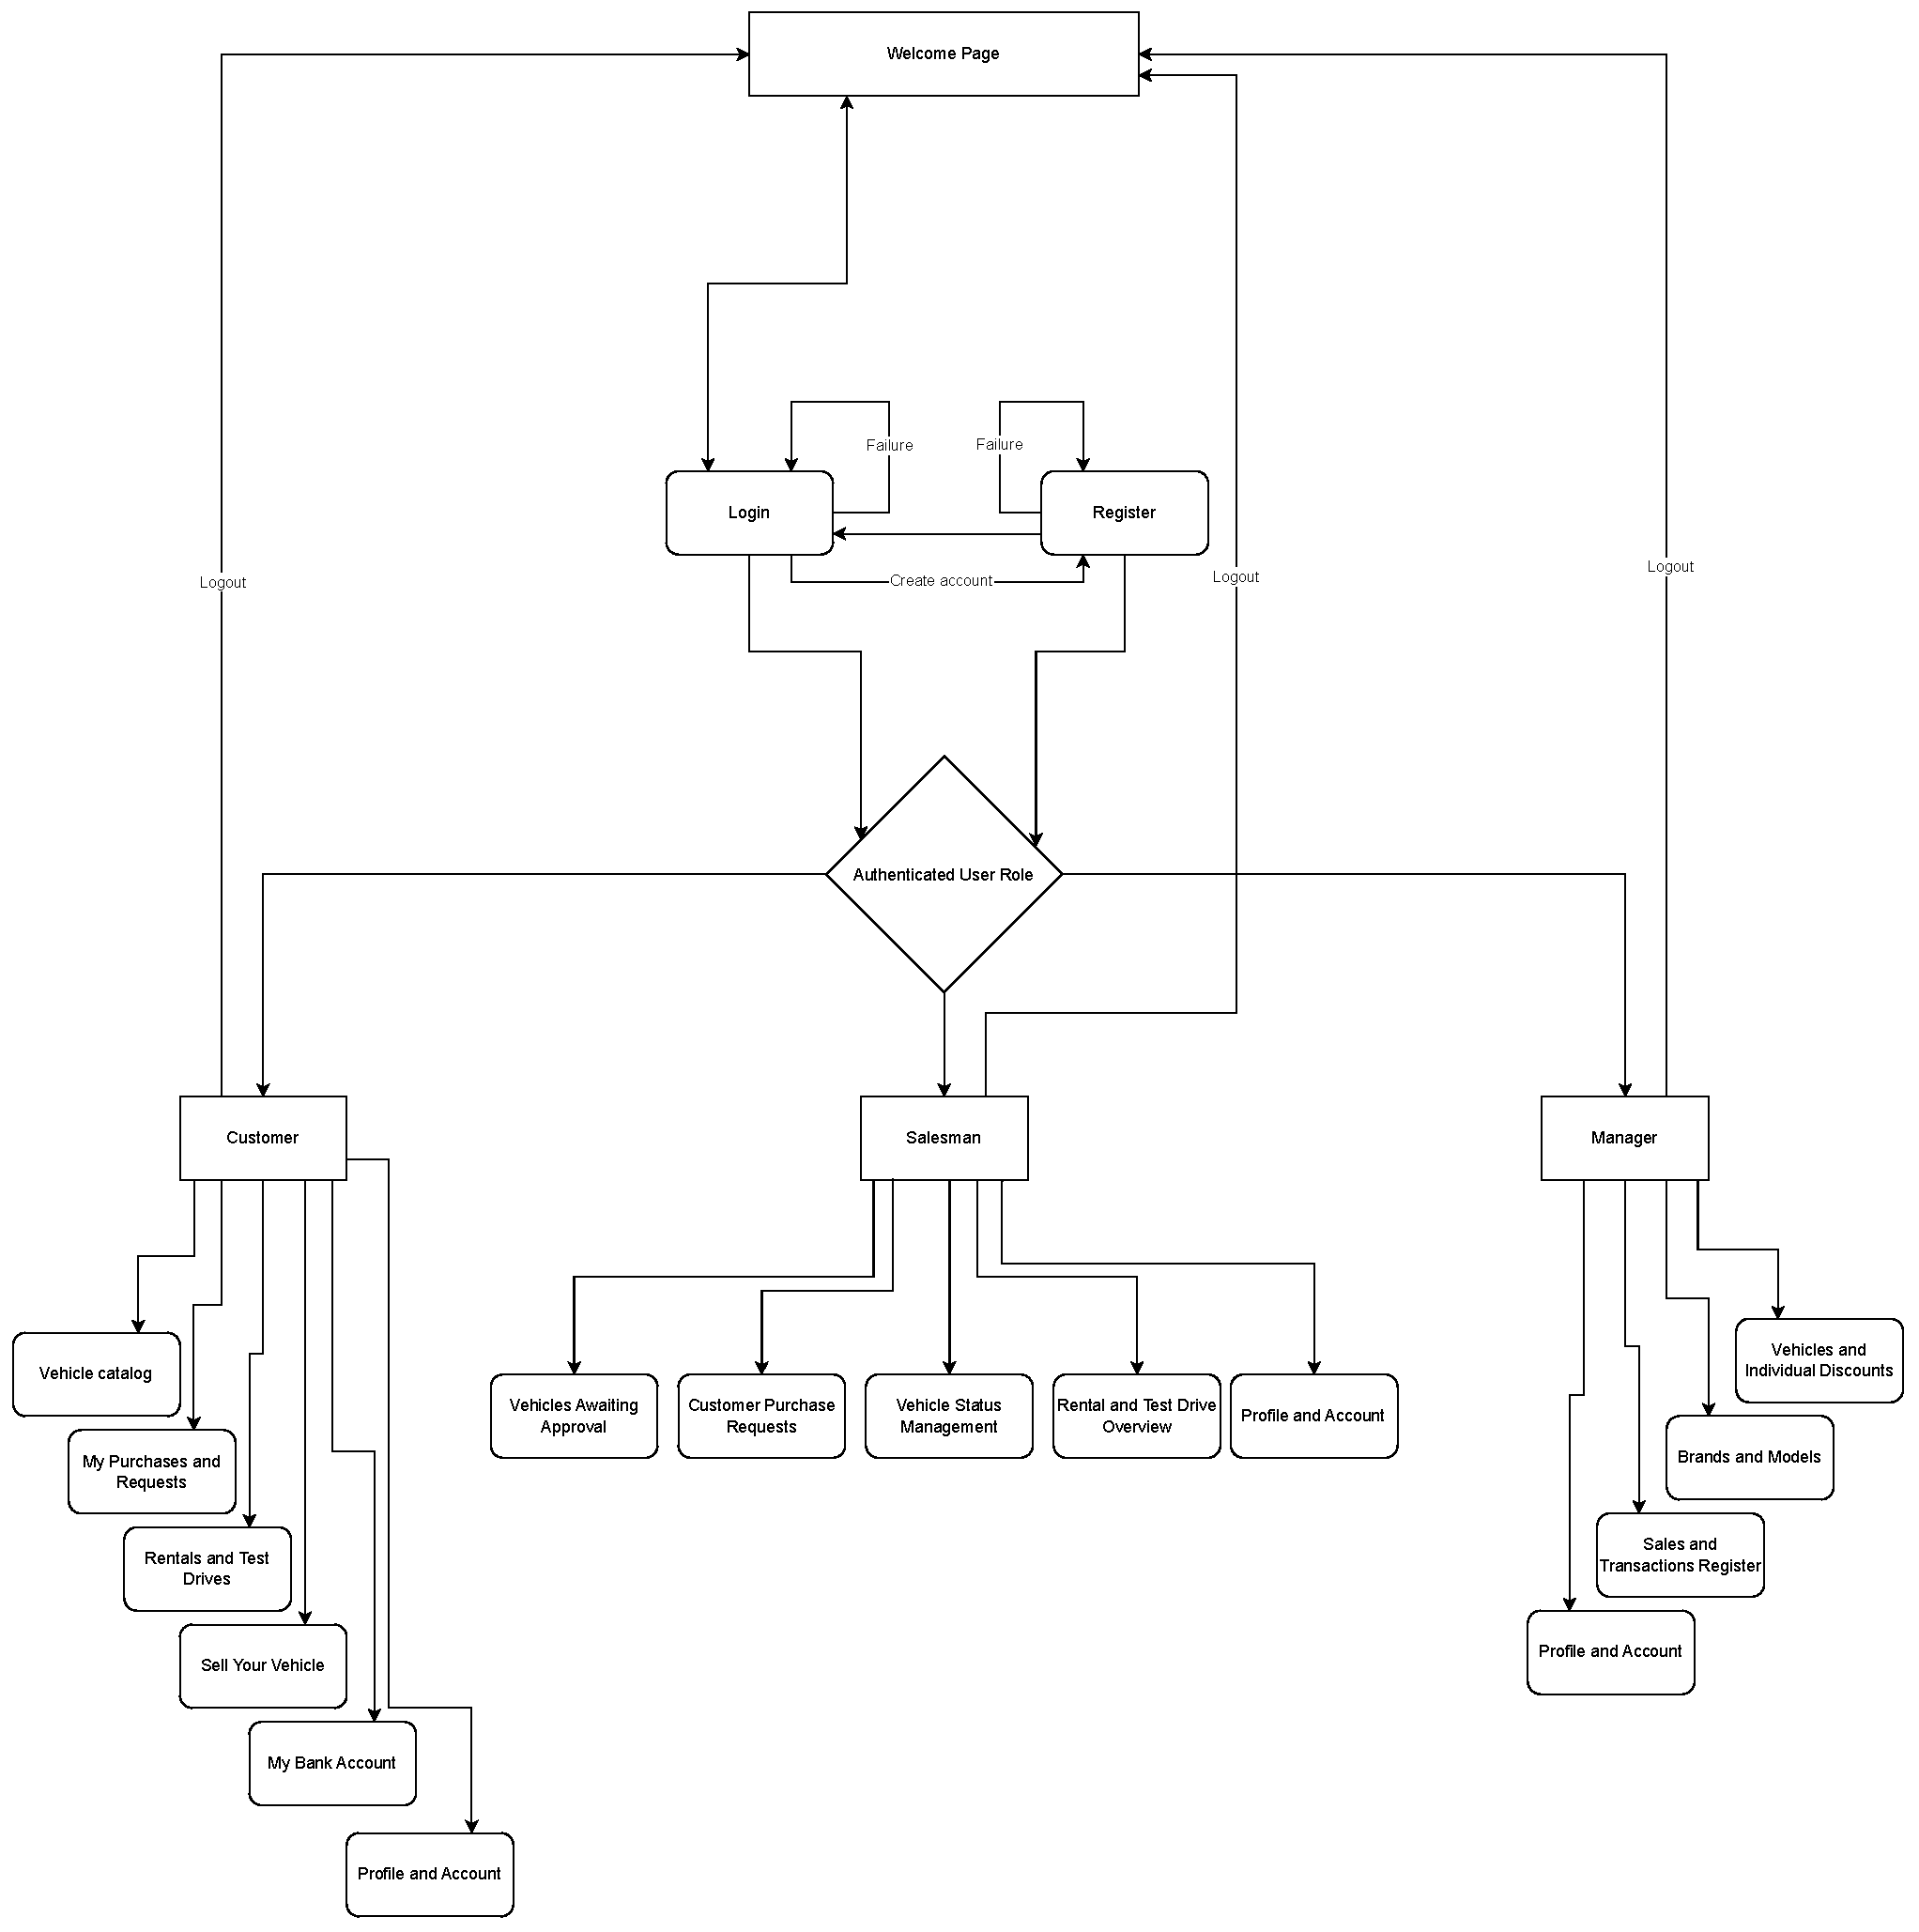
\includegraphics[width=\textwidth,height=.74\textheight,keepaspectratio]{page-navigation-original.pdf}
  \caption{Diagramma di navigazione delle pagine e delle schede di DriveHub.}\label{fig:navigazione-corrente}
\end{figure}

\clearpage
\section{Package Diagram}\label{sec:package-diagram}

Il codice di DriveHub è organizzato sotto il package radice \code{it.unifi.ing.drivehub} in quattro parti principali. \code{presentation} gestisce le schermate JavaFX, i controller e la navigazione; \code{business} coordina i casi d'uso e le strategie di calcolo; \code{dao} definisce le interfacce di persistenza e le implementa tramite JDBC; \code{domain} raccoglie le entità e le regole proprie dei veicoli e delle operazioni. Le frecce del diagramma indicano la direzione delle dipendenze: i servizi usano le interfacce DAO, l'implementazione PostgreSQL usa quelle interfacce e le entità, mentre il dominio non dipende dagli altri tre livelli.

\begin{figure}[H]
  \centering
  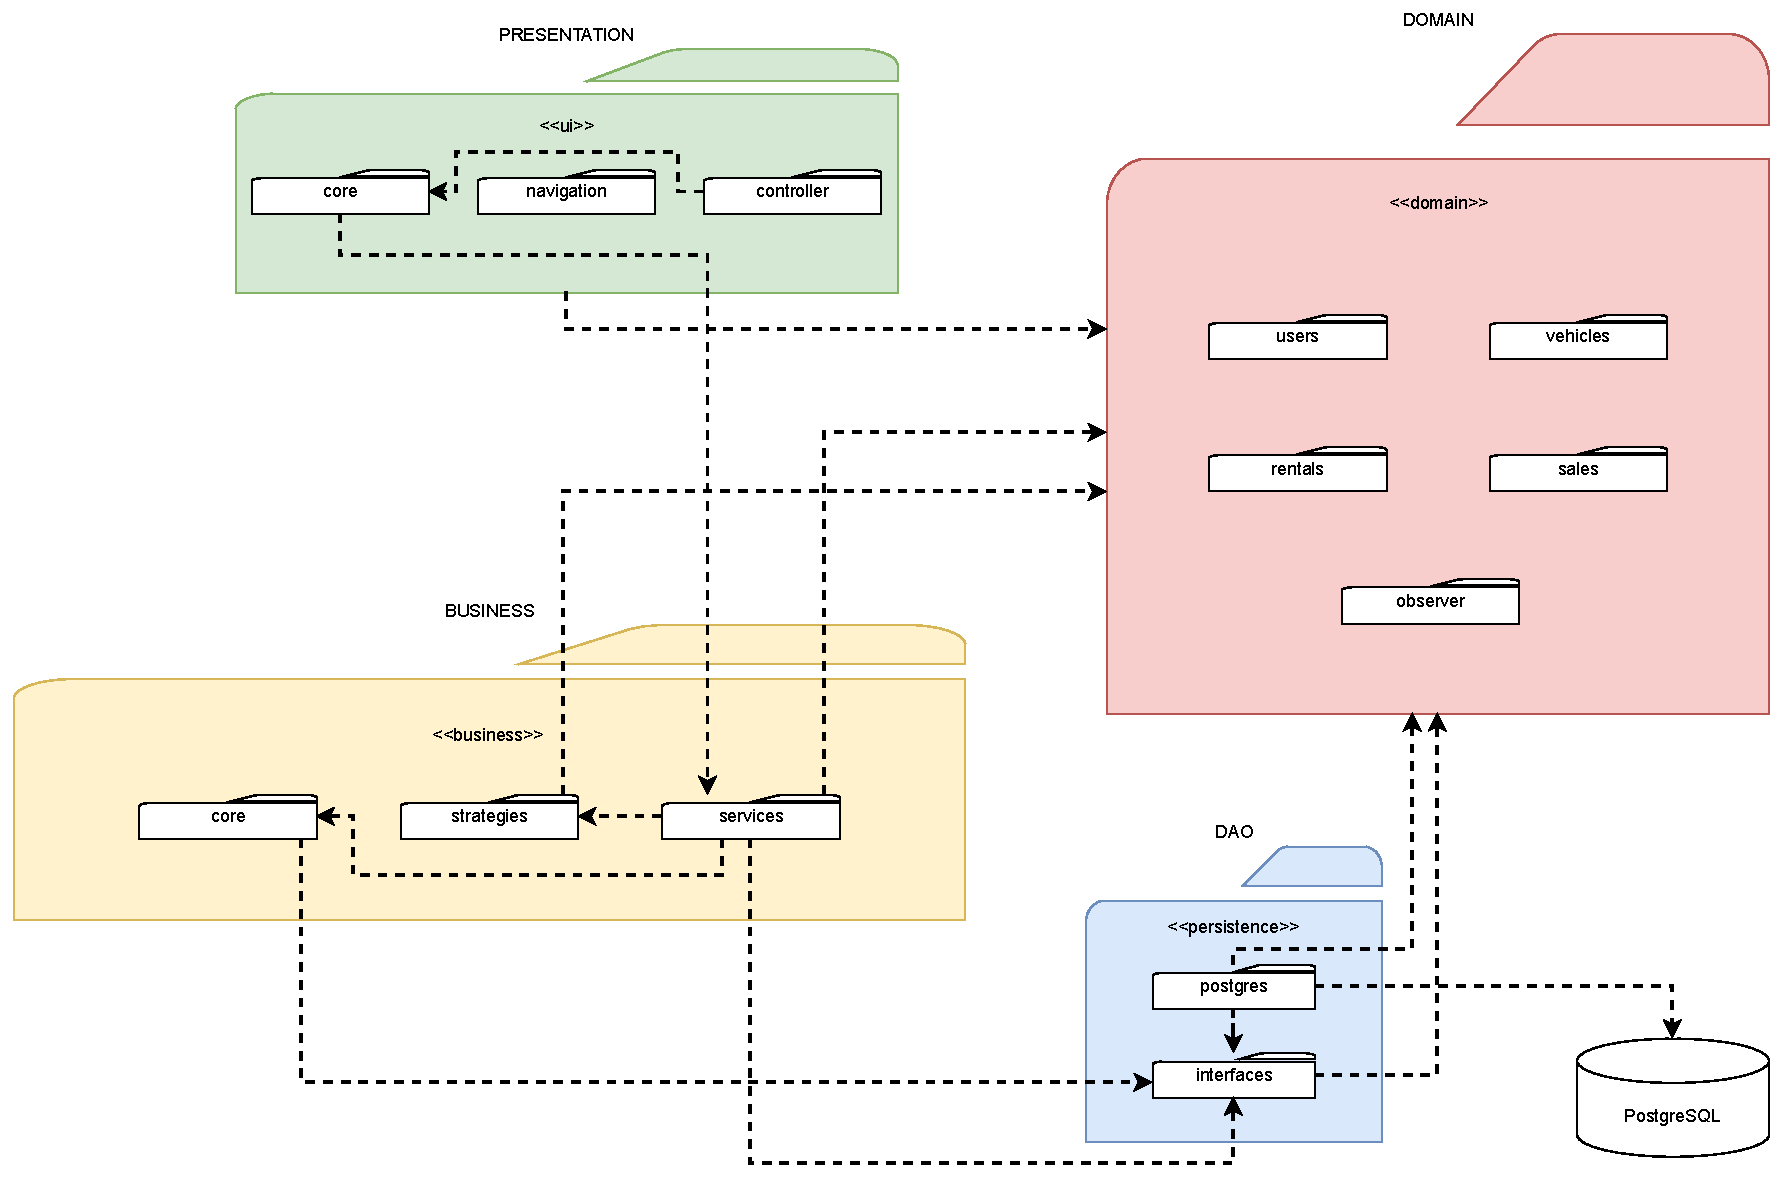
\includegraphics[width=.95\textwidth,height=.68\textheight,keepaspectratio]{package-diagram-original.pdf}
  \caption{Diagramma dei package di DriveHub e delle loro dipendenze.}\label{fig:package-attuale}
\end{figure}

\subsection*{Il dominio non dipende dagli altri livelli}

Le classi del package \code{domain} non importano classi di \code{presentation}, \code{business} o \code{dao}: le entità non conoscono né le schermate né il modo in cui vengono salvate. Nel diagramma le dipendenze entrano nel dominio, senza frecce in uscita verso gli altri livelli. Questa separazione permette di applicare e verificare le regole delle entità indipendentemente dall'interfaccia JavaFX e da PostgreSQL.

La separazione ha un effetto concreto in \code{Vehicle}: i metodi \code{approve}, \code{block} e \code{unblock} controllano lo stato corrente prima di modificarlo, senza affidare questa regola al controller o al DAO. Anche \code{BankAccount} verifica nel dominio che un prelievo non superi il saldo disponibile. I servizi coordinano queste operazioni; le condizioni proprie delle entità restano nelle classi che le rappresentano. Nel disegno le frecce \code{controller} $\rightarrow$ \code{presentation.core} e \code{presentation.core} $\rightarrow$ \code{business.services} rispecchiano il passaggio dai controller a \code{UiGateway} e poi a \code{ServiceUiGateway}, che invoca i servizi.

\clearpage
\section{Class Diagram}\label{sec:class-diagram}

Il diagramma dei package della sezione~\ref{sec:package-diagram} è dettagliato in quattro diagrammi di classe. Le figure mantengono i colori dei livelli e riportano i membri essenziali alla lettura delle dipendenze.

\subsection{Domain Model}

Il dominio comprende catalogo, utenti, operazioni ed eventi di inventario. \code{Vehicle} controlla alcune transizioni di stato e \code{BankAccount} verifica il saldo nei prelievi. \code{User}, \code{Vehicle}, \code{Request}, \code{Sale}, \code{Rent} e \code{TestDrive} derivano da \code{BaseEntity}; nel disegno compaiono solo tre generalizzazioni per evitare sovrapposizioni. I riferimenti fra entità usano ID, non associazioni Java dirette. \code{Vehicle.transitionTo} consente anche cambi di stato generici.

\begin{figure}[H]
  \centering
  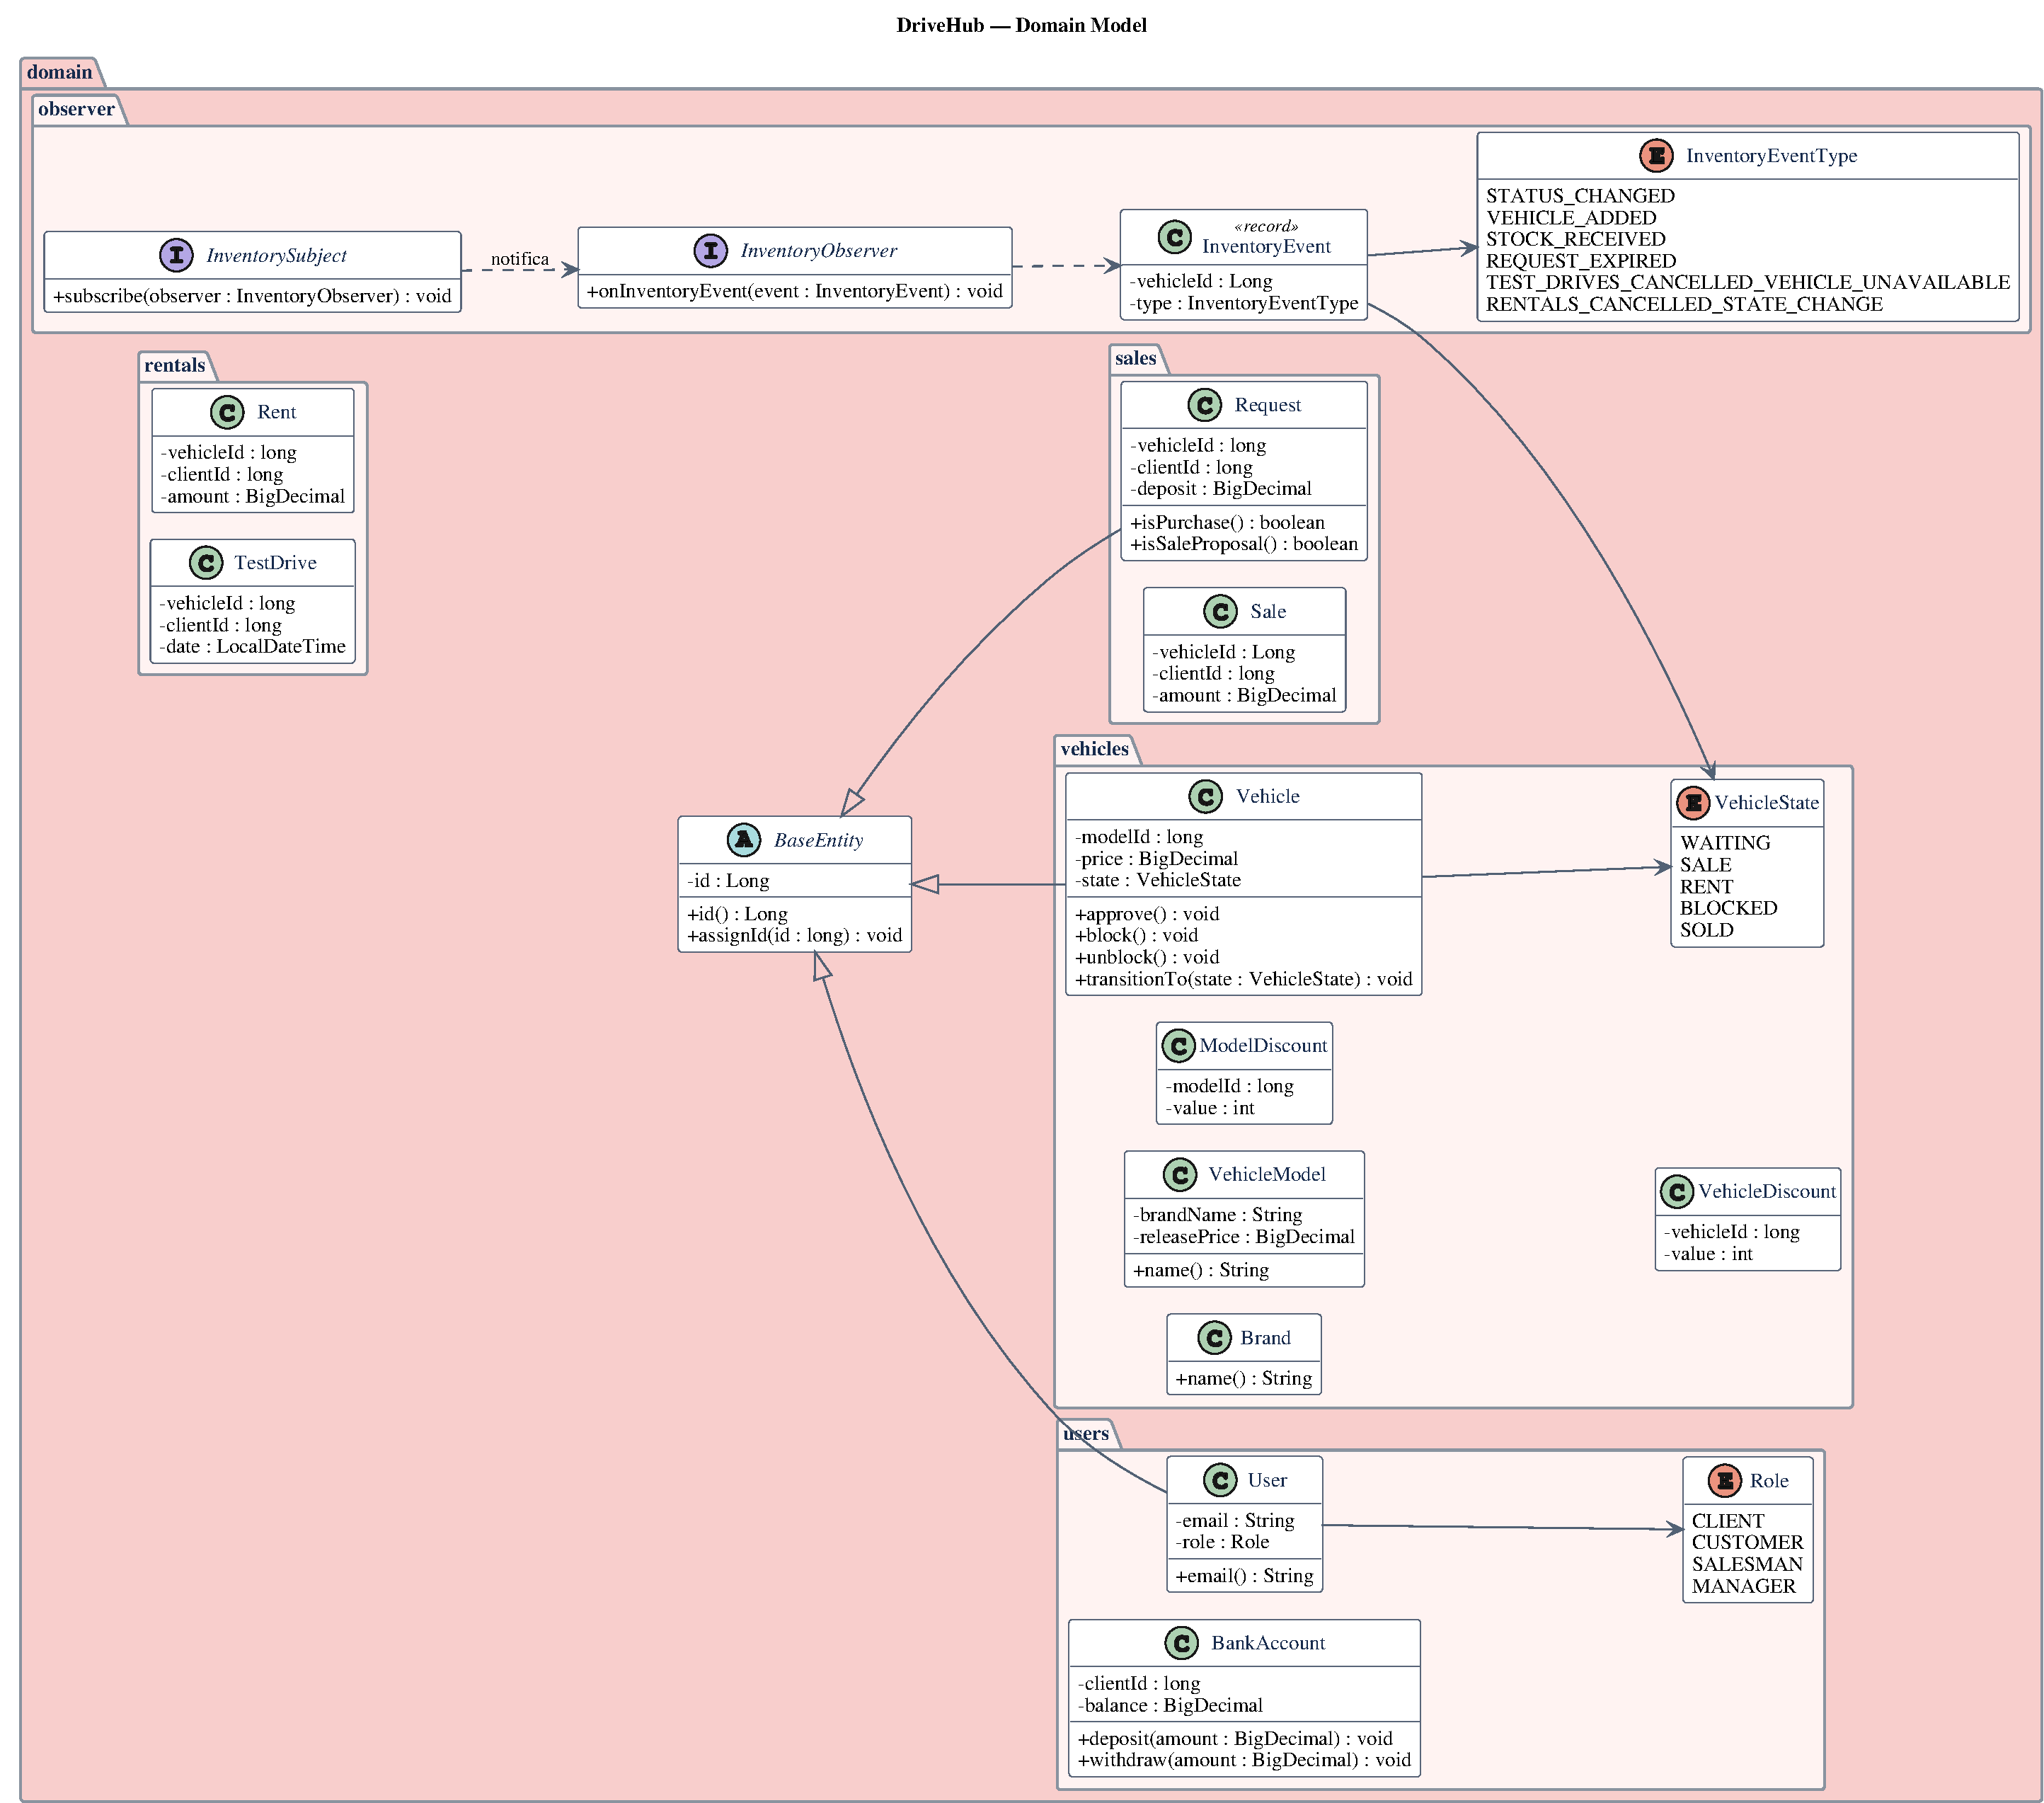
\includegraphics[width=\textwidth,height=.59\textheight,keepaspectratio]{class-domain-drivehub.pdf}
  \caption{Domain Model di DriveHub: classi rappresentative dei package interni al dominio.}\label{fig:classi-domain}
\end{figure}

\clearpage
\subsection{Business Layer}

I servizi coordinano i casi d'uso dell'applicazione. \code{TransactionRunner} apre una \code{UnitOfWork} tramite \code{DaoFactory}, così le operazioni correlate possono condividere una transazione. \code{PricingService} delega i calcoli a \code{PricingStrategy}, implementata da \code{StandardPricingStrategy}; \code{AuthService} usa \code{PasswordHasher} per le credenziali. \code{SalesService} e \code{RentalService} implementano \code{InventorySubject} e notificano gli \code{InventoryObserver}. Nel diagramma le piccole aree blu e rosse mostrano le interfacce degli altri livelli usate dal business.

\begin{figure}[H]
  \centering
  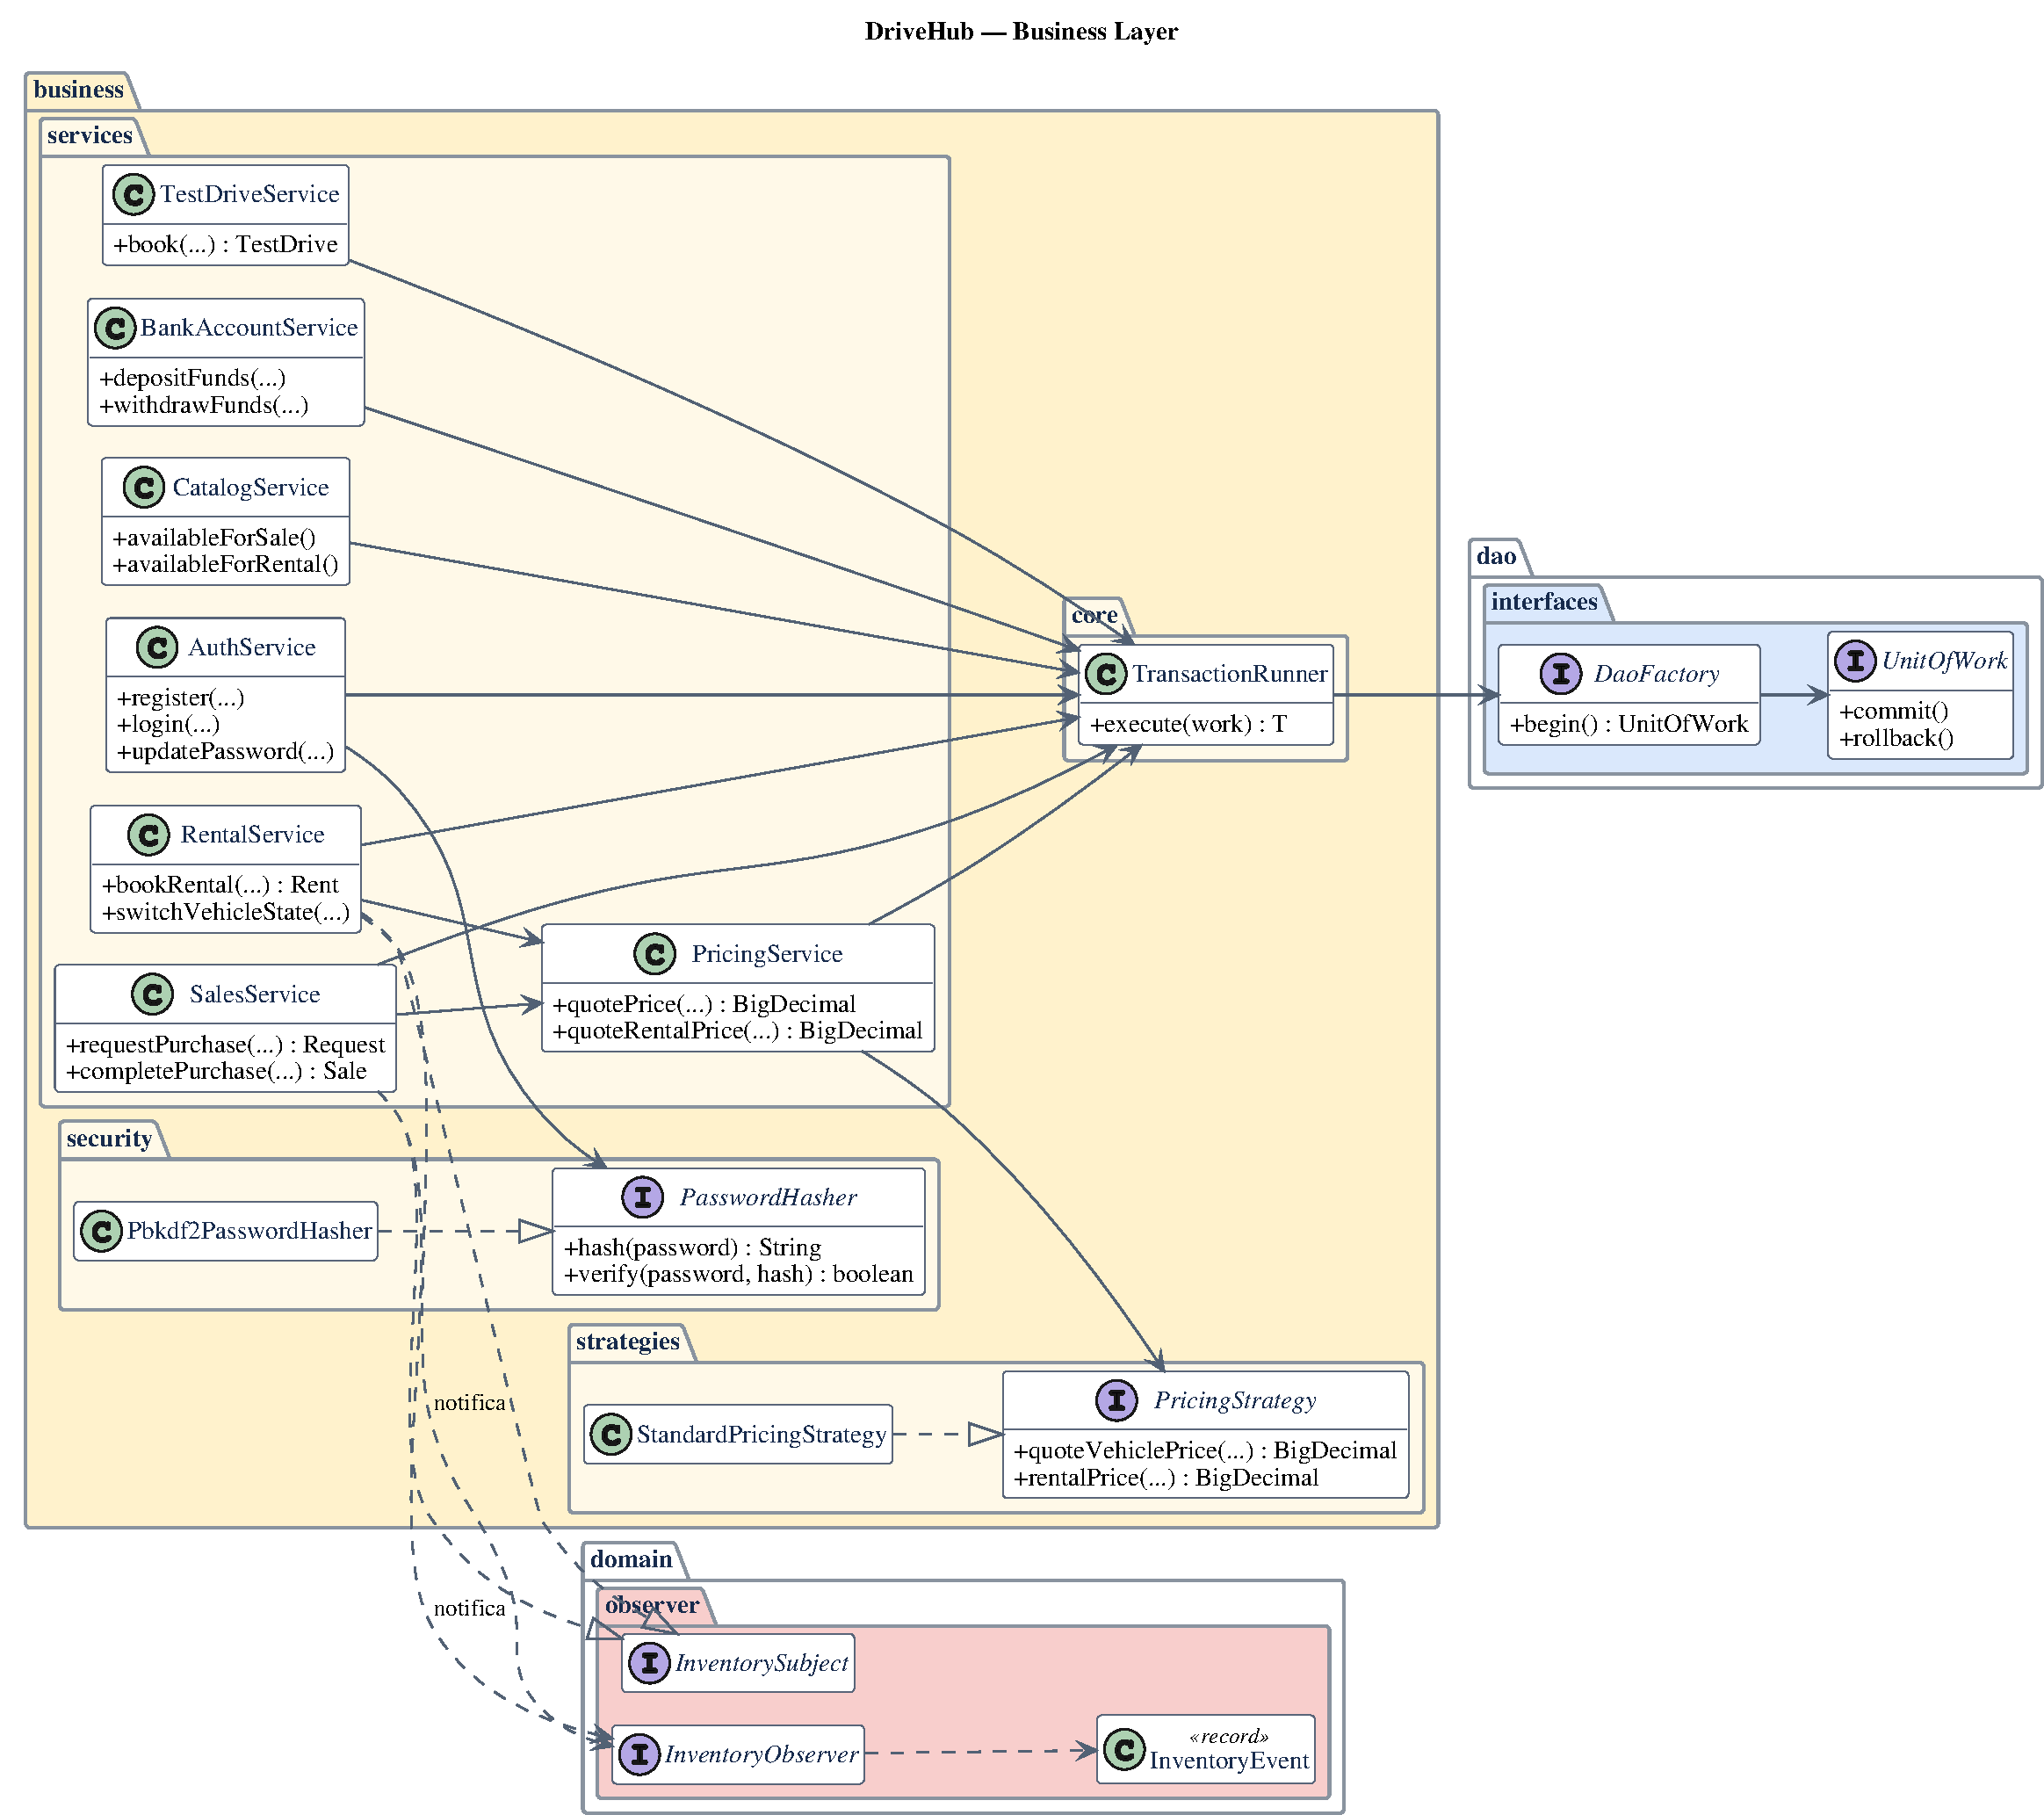
\includegraphics[width=\textwidth,height=.72\textheight,keepaspectratio]{class-business-drivehub.pdf}
  \caption{Business Layer: servizi, transazioni, Strategy e Observer.}\label{fig:classi-business}
\end{figure}

\clearpage
\subsection{DAO}

Il DAO separa le porte di persistenza dalle classi che eseguono le query JDBC. \code{PostgresDaoFactory.begin} crea una \code{PostgresUnitOfWork}; questa espone i DAO che condividono la connessione e offre \code{commit} e \code{rollback}. Il diagramma mostra quattro coppie interfaccia--implementazione come esempio. Le altre sei porte, per conti, marchi, modelli, sconti, test drive e vendite, seguono lo stesso schema. \code{JdbcEntityLoader} collabora alla ricostruzione degli oggetti dai risultati SQL.

\begin{figure}[H]
  \centering
  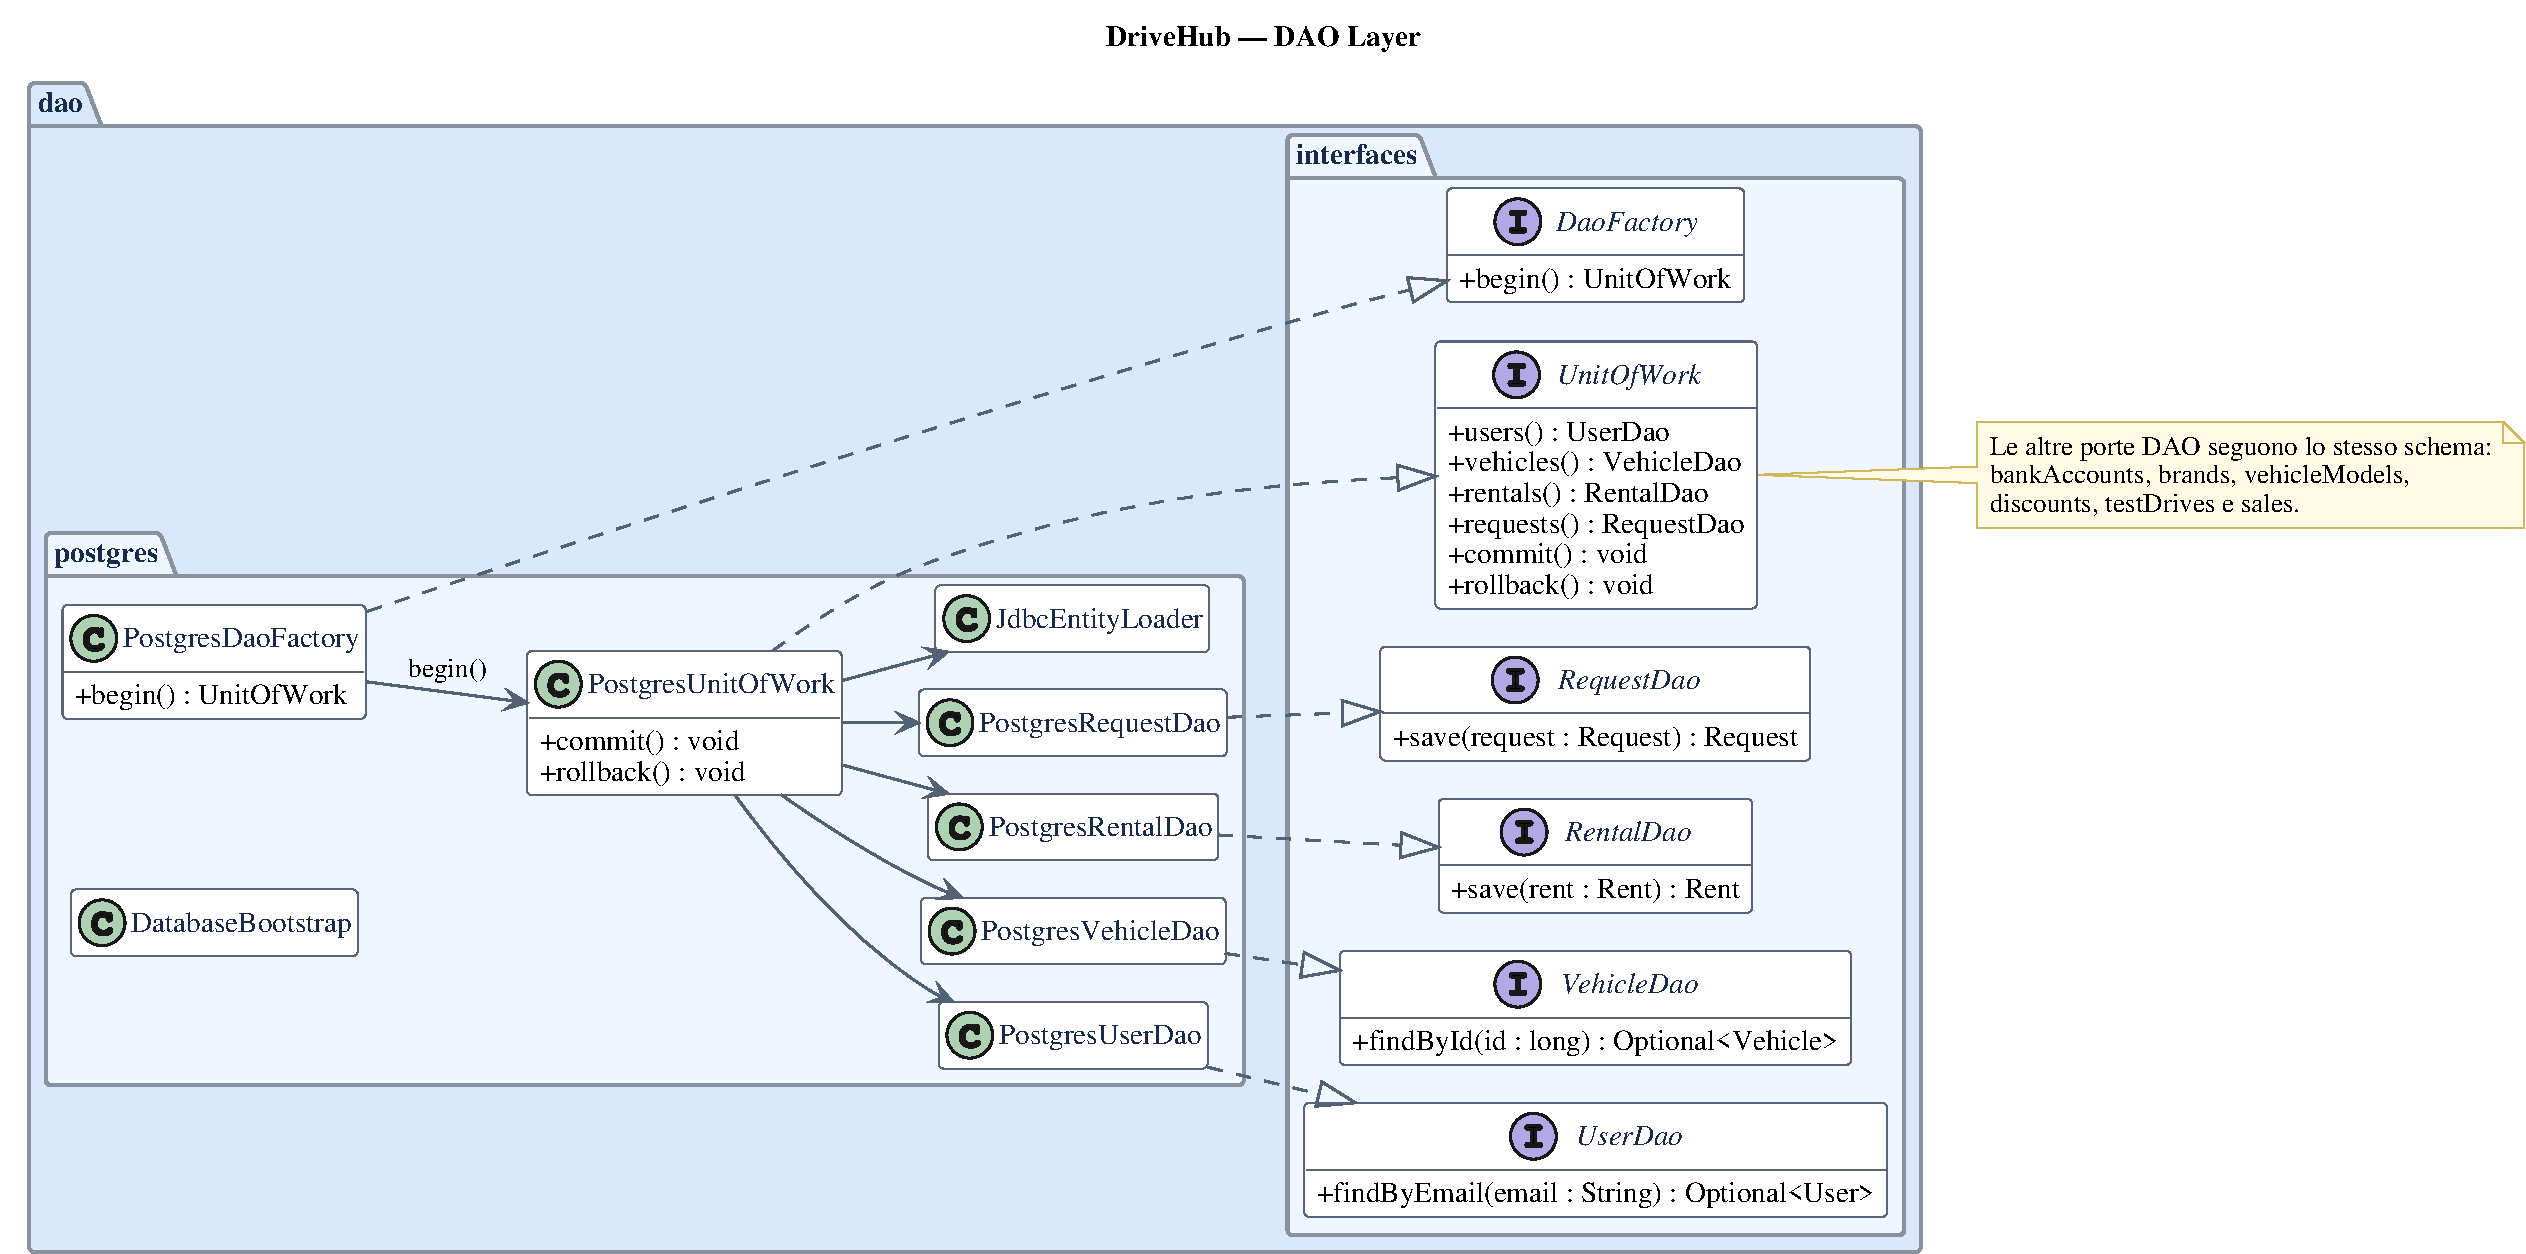
\includegraphics[width=\textwidth,height=.72\textheight,keepaspectratio]{class-dao-drivehub.pdf}
  \caption{DAO: porte, factory, unità di lavoro e implementazioni PostgreSQL rappresentative.}\label{fig:classi-dao}
\end{figure}

\clearpage
\subsection{Presentation Layer}

La presentazione raccoglie i controller JavaFX, il contesto applicativo, il gateway e la navigazione. I controller dei tre ruoli, del login e della registrazione estendono \code{AbstractController}, che riceve \code{ApplicationContext} e permette l'accesso a \code{UiGateway} e alla sessione. \code{ServiceUiGateway} implementa il gateway, invoca i servizi e restituisce i record di \code{UiModels}. \code{NavigationManager} carica le schermate individuate da \code{Route} e passa il contesto ai controller; \code{WelcomeController} è una classe separata, senza ereditarietà da \code{AbstractController}. Il controllo dei ruoli in \code{Route} riguarda la navigazione e non costituisce, da solo, un'autorizzazione di tutte le operazioni applicative.

\begin{figure}[H]
  \centering
  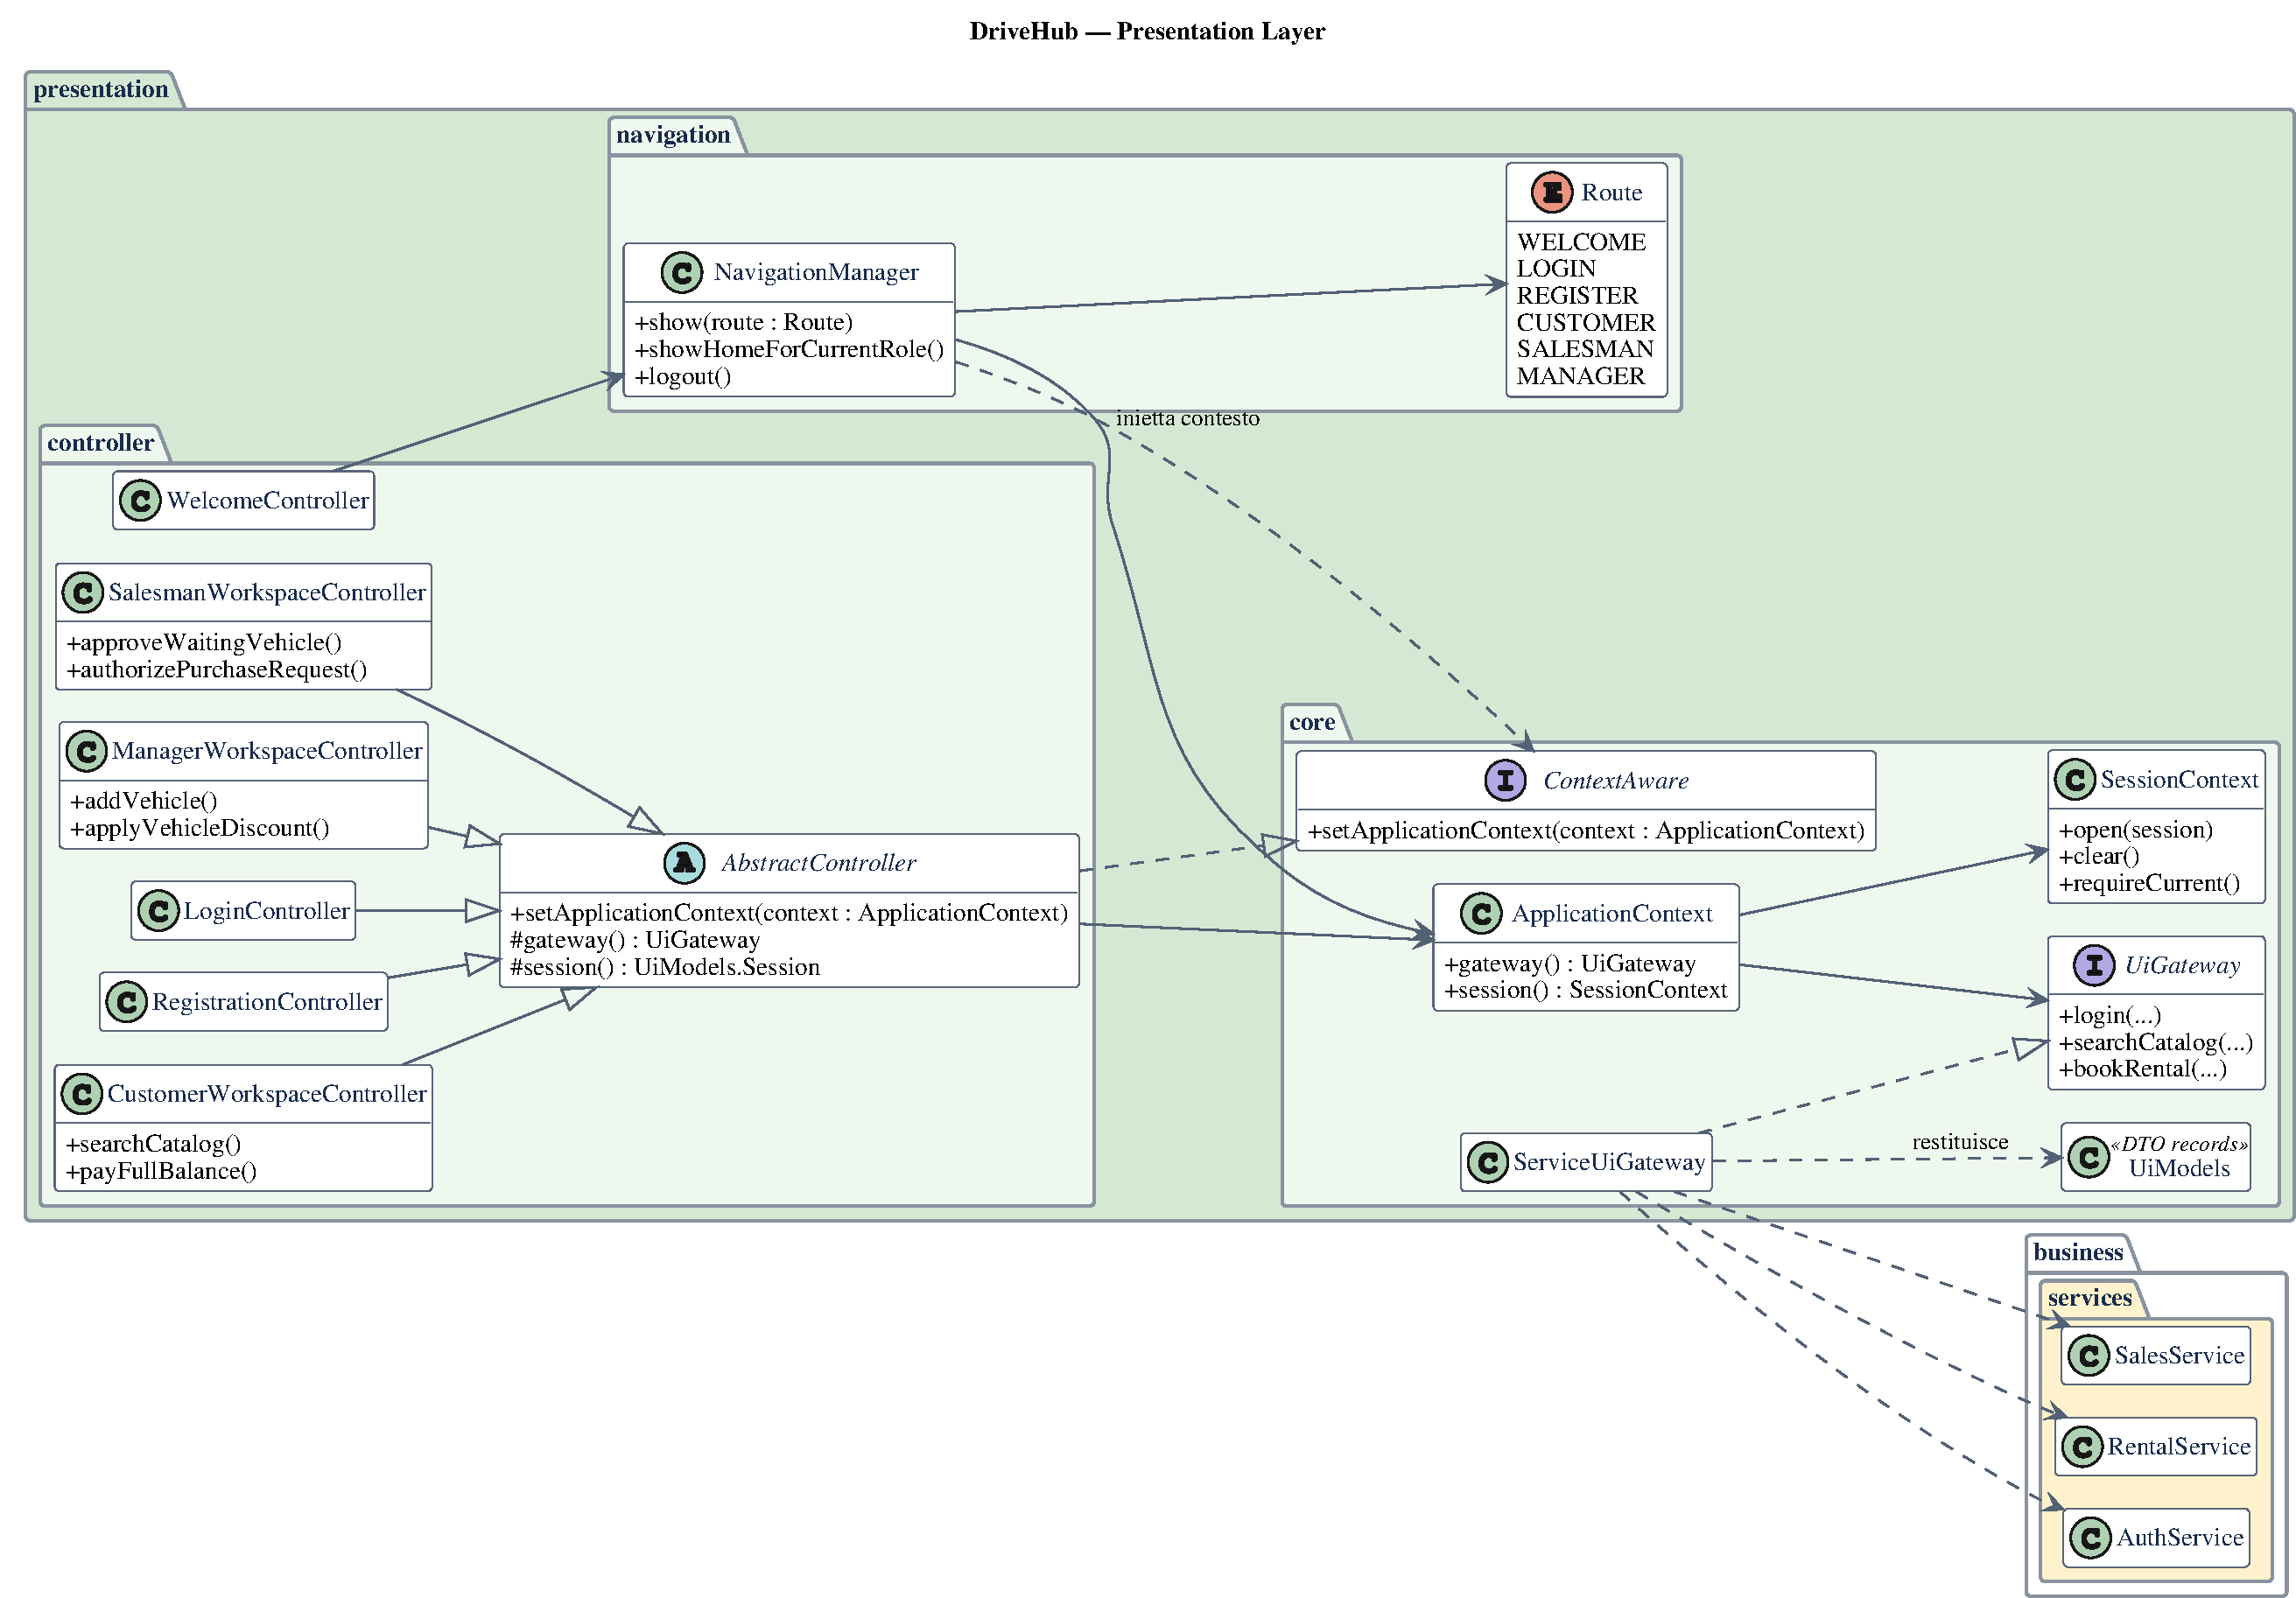
\includegraphics[width=\textwidth,height=.72\textheight,keepaspectratio]{class-presentation-drivehub.pdf}
  \caption{Presentation Layer: controller, gateway, sessione e navigazione.}\label{fig:classi-presentation}
\end{figure}

\section{Sequence Diagram}\label{sec:sequenze}

I diagrammi di sequenza descrivono tre flussi significativi di DriveHub e mostrano come presentazione, servizi, dominio e persistenza collaborano nel tempo. Le chiamate ai servizi partono dai controller JavaFX e attraversano \code{ServiceUiGateway}: nel diagramma dell'acquisizione il gateway ha una linea di vita, mentre negli altri due è indicato in una nota. La linea «UnitOfWork / DAO» raccoglie l'apertura della transazione tramite \code{DaoFactory}, le chiamate ai DAO sulla stessa connessione e il commit. I diagrammi sono stati disegnati selezionando le operazioni effettive nei metodi di servizio, non generati automaticamente dai sorgenti.

\subsection{Acquisto di un veicolo}

\begin{figure}[H]
  \centering
  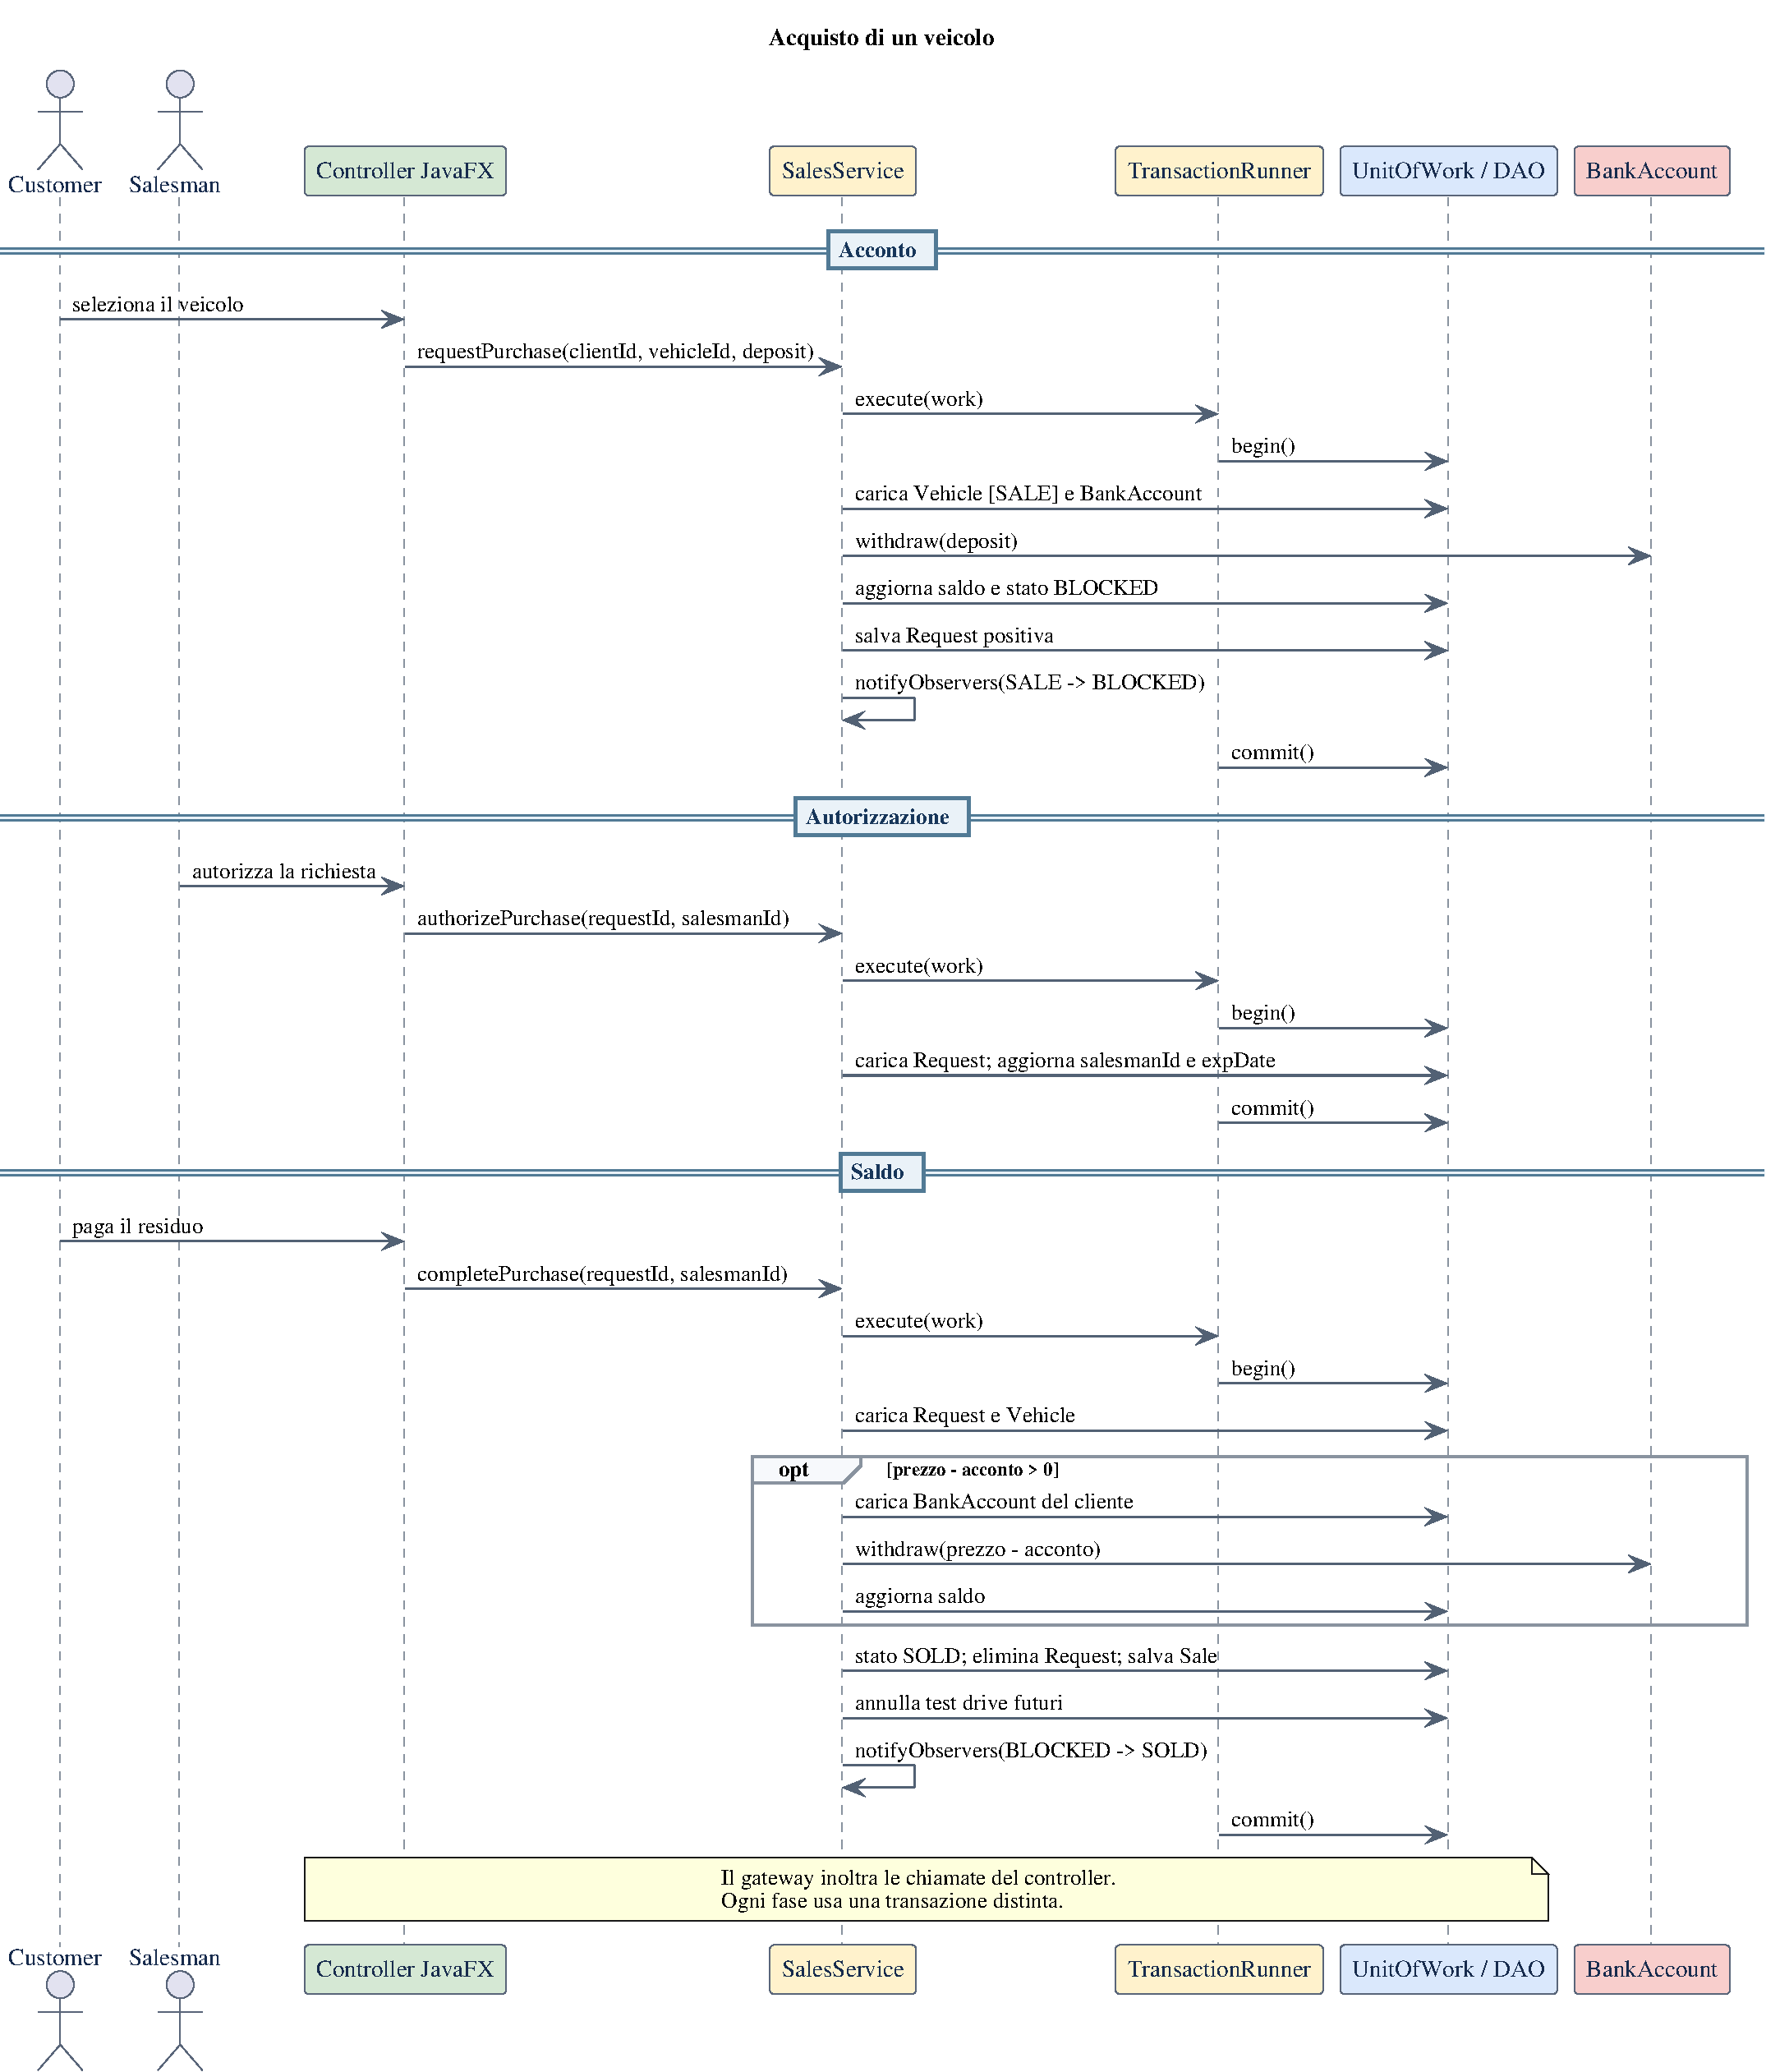
\includegraphics[width=\textwidth,height=.72\textheight,keepaspectratio]{sequence-purchase-drivehub.pdf}
  \caption{Acquisto: acconto del Customer, autorizzazione del Salesman e saldo finale.}\label{fig:seq-purchase}
\end{figure}

La figura~\ref{fig:seq-purchase} distingue tre transazioni. La prima verifica lo stato \code{SALE}, addebita l'acconto sul conto dimostrativo, porta il veicolo a \code{BLOCKED} e salva una \code{Request} positiva. Il Salesman imposta poi il proprio ID e una scadenza di un mese. Infine \code{SalesService} addebita al cliente della richiesta il residuo (prezzo meno acconto), registra la \code{Sale}, elimina la \code{Request} e annulla i test drive futuri prima del commit. Il controller abilita il saldo dopo l'autorizzazione, ma \code{completePurchase} non ricontrolla scadenza né identità del chiamante.

\clearpage
\subsection{Prenotazione di un noleggio}

\begin{figure}[H]
  \centering
  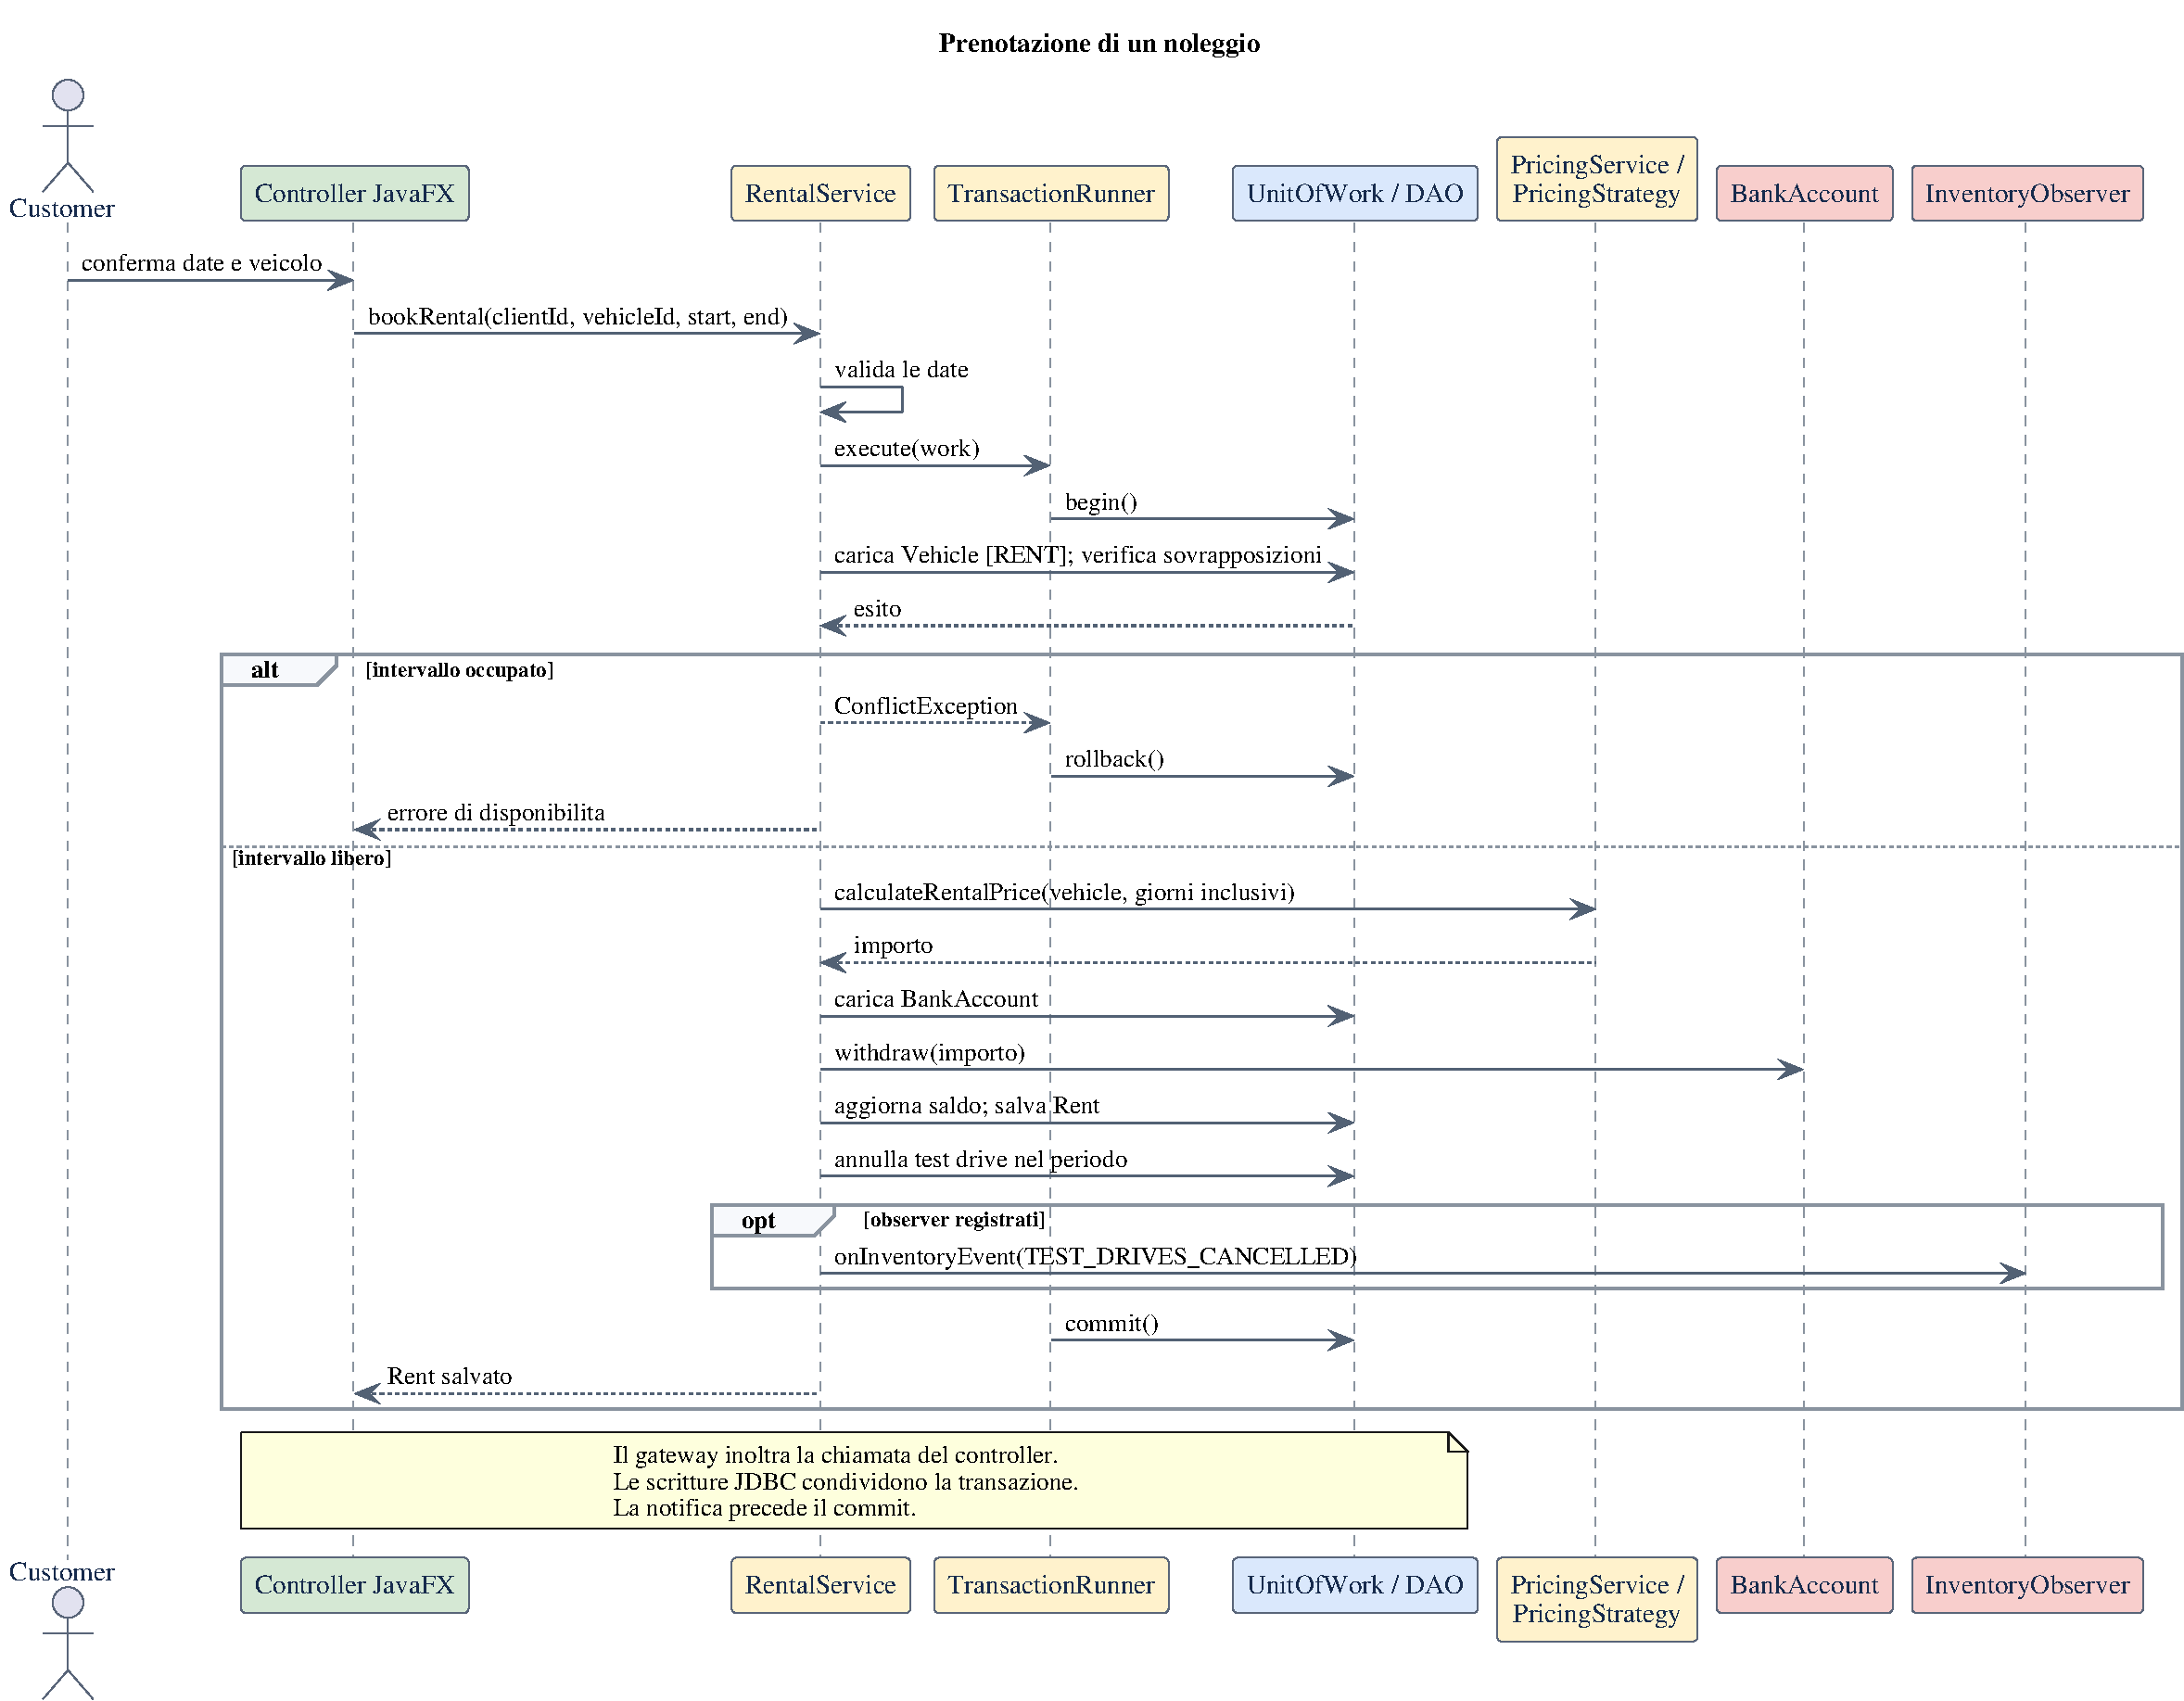
\includegraphics[width=\textwidth,height=.72\textheight,keepaspectratio]{sequence-rental-drivehub.pdf}
  \caption{Noleggio: controllo delle date, prezzo, addebito e registrazione nella stessa transazione.}\label{fig:seq-rental}
\end{figure}

La figura~\ref{fig:seq-rental} segue \code{RentalService.bookRental}. Il servizio valida le date, richiede che il veicolo sia in stato \code{RENT} e interroga il DAO per cercare noleggi sovrapposti. Se trova un conflitto, \code{TransactionRunner} esegue il rollback e la prenotazione non viene salvata. Nel percorso valido \code{PricingService} usa la \code{PricingStrategy} per calcolare l'importo sui giorni inclusivi; quindi il servizio addebita il conto dimostrativo, salva \code{Rent} e cancella i test drive nel periodo. La notifica a eventuali \code{InventoryObserver} precede il commit e non ha la stessa atomicità delle scritture JDBC. Il controllo di sovrapposizione è applicativo: nello schema non è presente un vincolo che escluda due prenotazioni concorrenti sullo stesso intervallo.

\clearpage
\subsection{Acquisizione di un veicolo del Customer}

\begin{figure}[H]
  \centering
  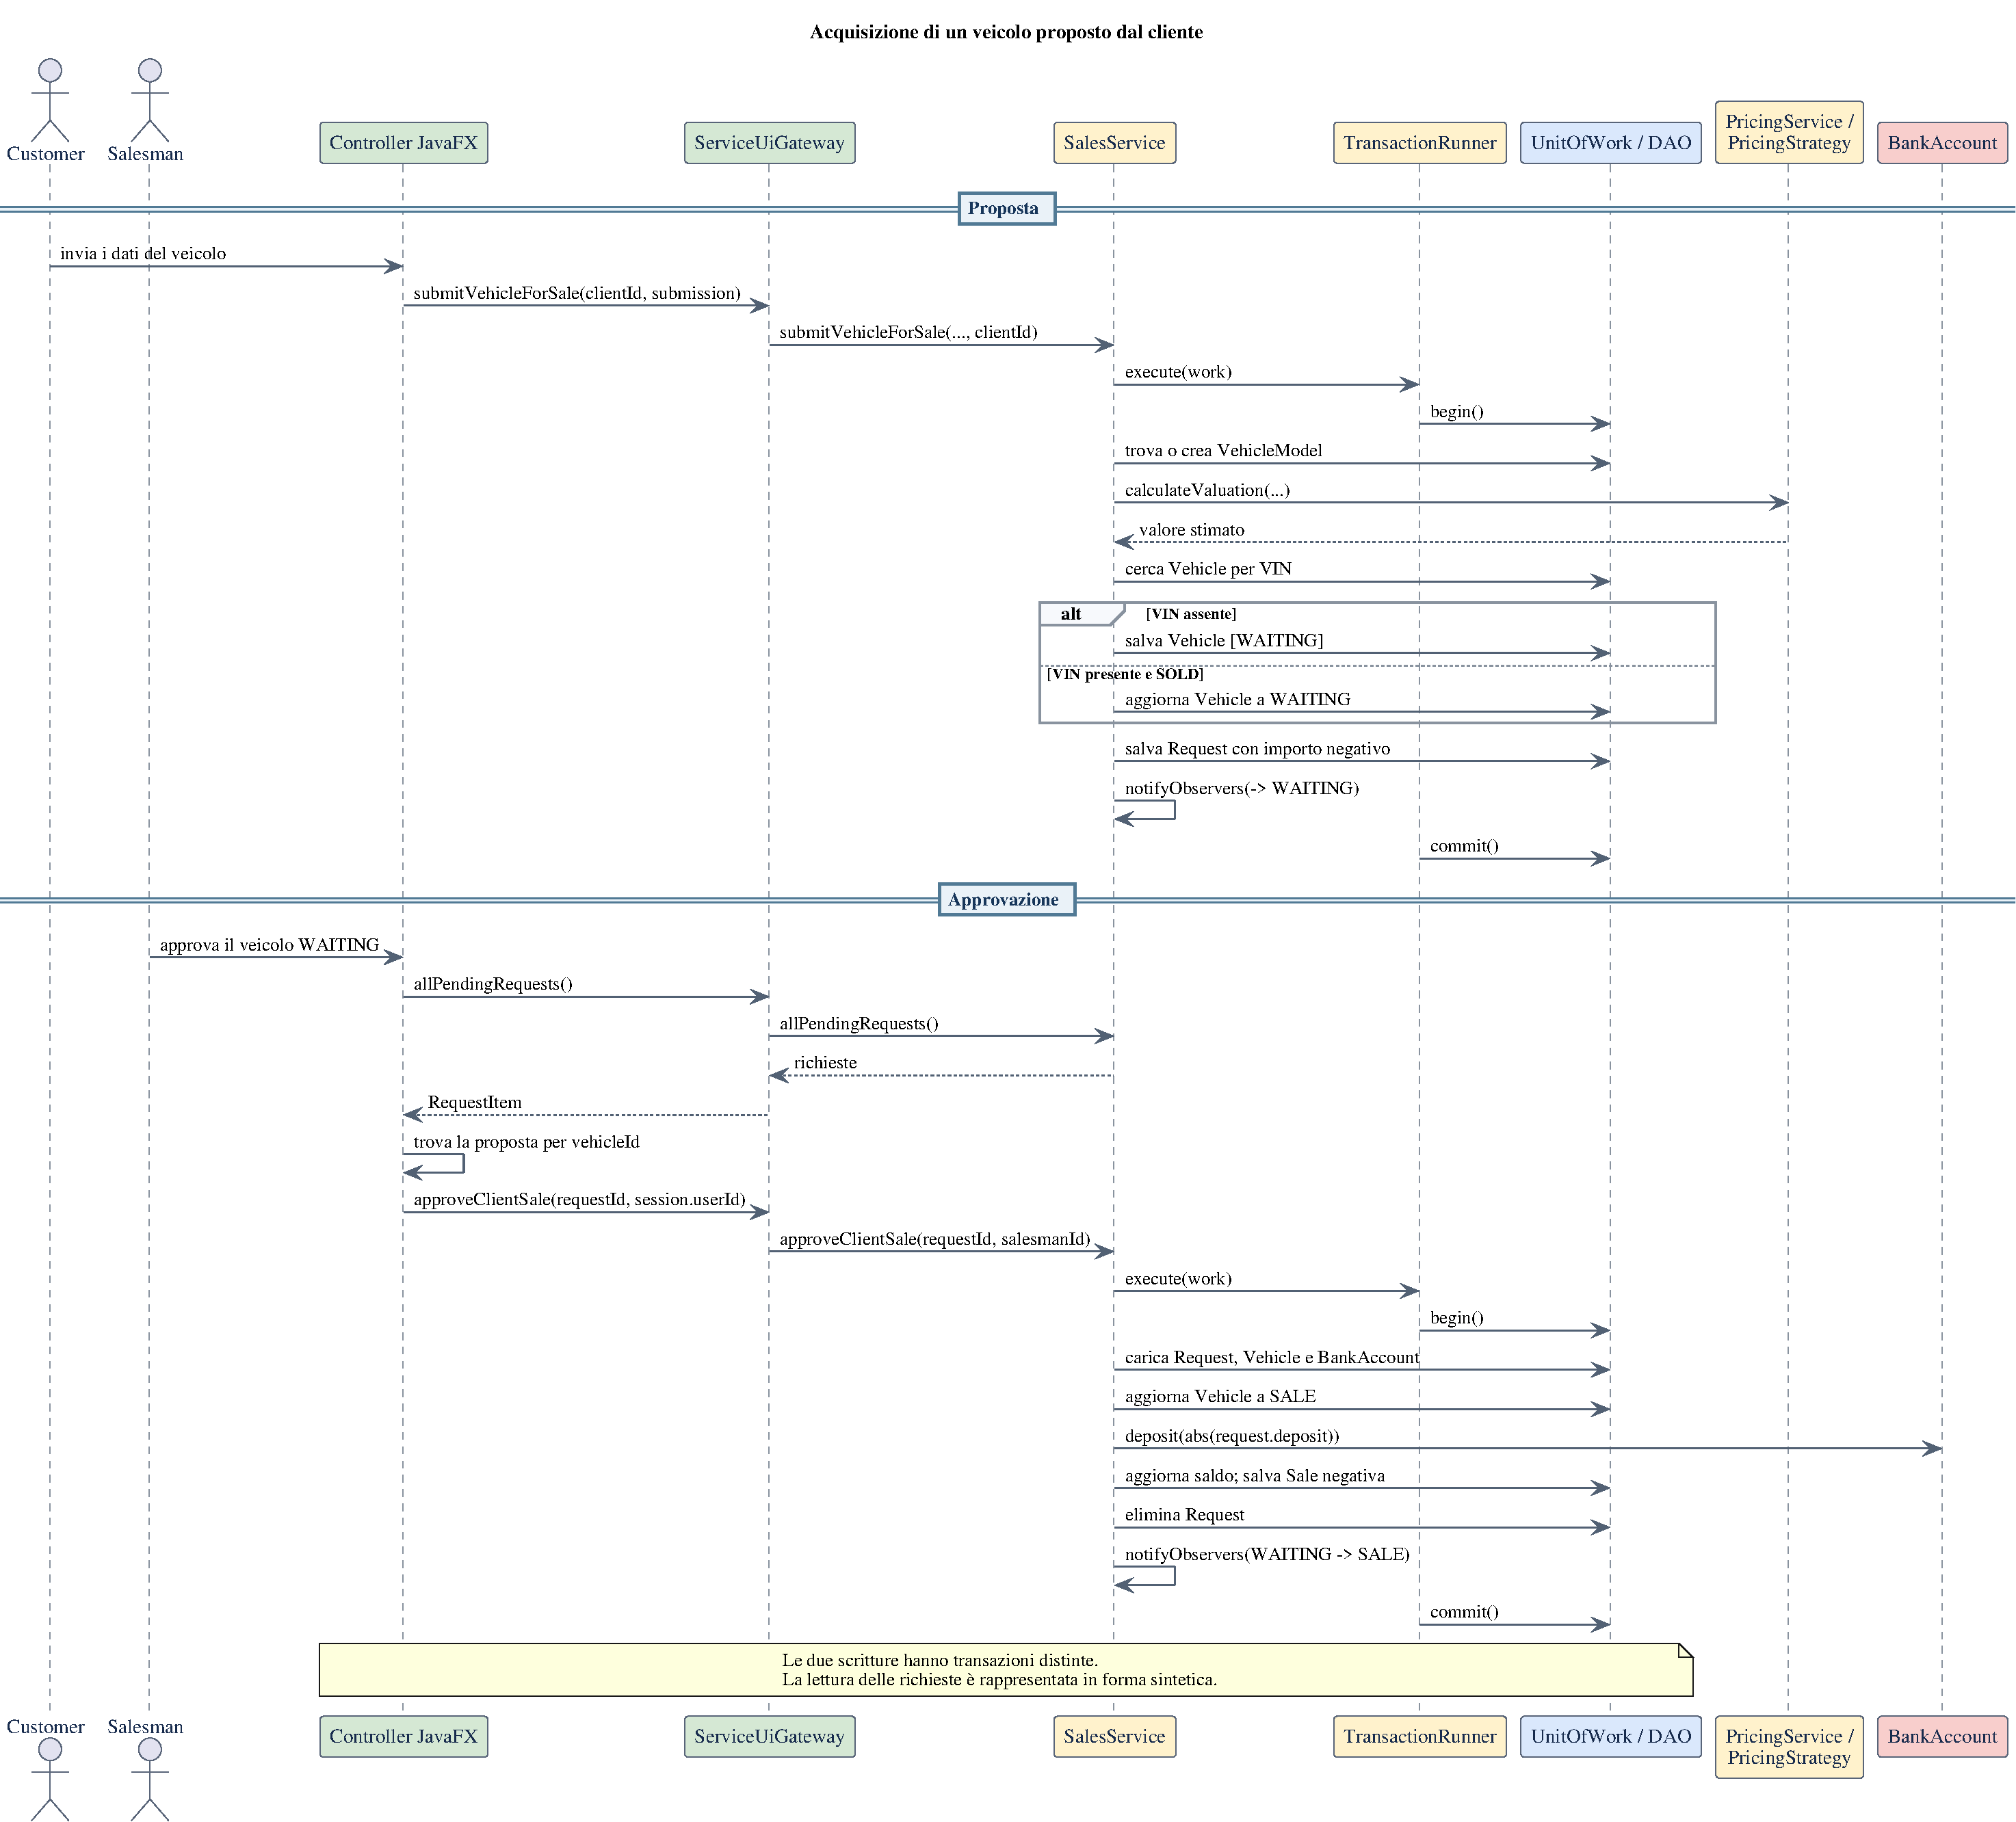
\includegraphics[width=\textwidth,height=.72\textheight,keepaspectratio]{sequence-acquisition-drivehub.pdf}
  \caption{Acquisizione: proposta del Customer e approvazione del Salesman, ciascuna in una transazione di scrittura.}\label{fig:seq-acquisition}
\end{figure}

Nella figura~\ref{fig:seq-acquisition}, la proposta crea o riusa un veicolo \code{SOLD}, lo pone in \code{WAITING} e salva una \code{Request} negativa. Il controller del Salesman cerca la richiesta di proposta per il veicolo selezionato e passa a \code{approveClientSale} l'ID del venditore in sessione. L'approvazione accredita il cliente, registra una \code{Sale} negativa, elimina la richiesta e porta il veicolo a \code{SALE} in una transazione. Il metodo \code{approveVehicle} è usato dal controller solo quando non trova una proposta; se chiamato direttamente su una proposta, apre invece due unità di lavoro annidate e usa l'ID venditore costante \code{1L}. La decisione appartiene al Salesman, non al Manager della specifica storica.

\clearpage
\section{Database}\label{sec:dati}

\subsection{Schema ER}
\begin{figure}[H]
  \centering
  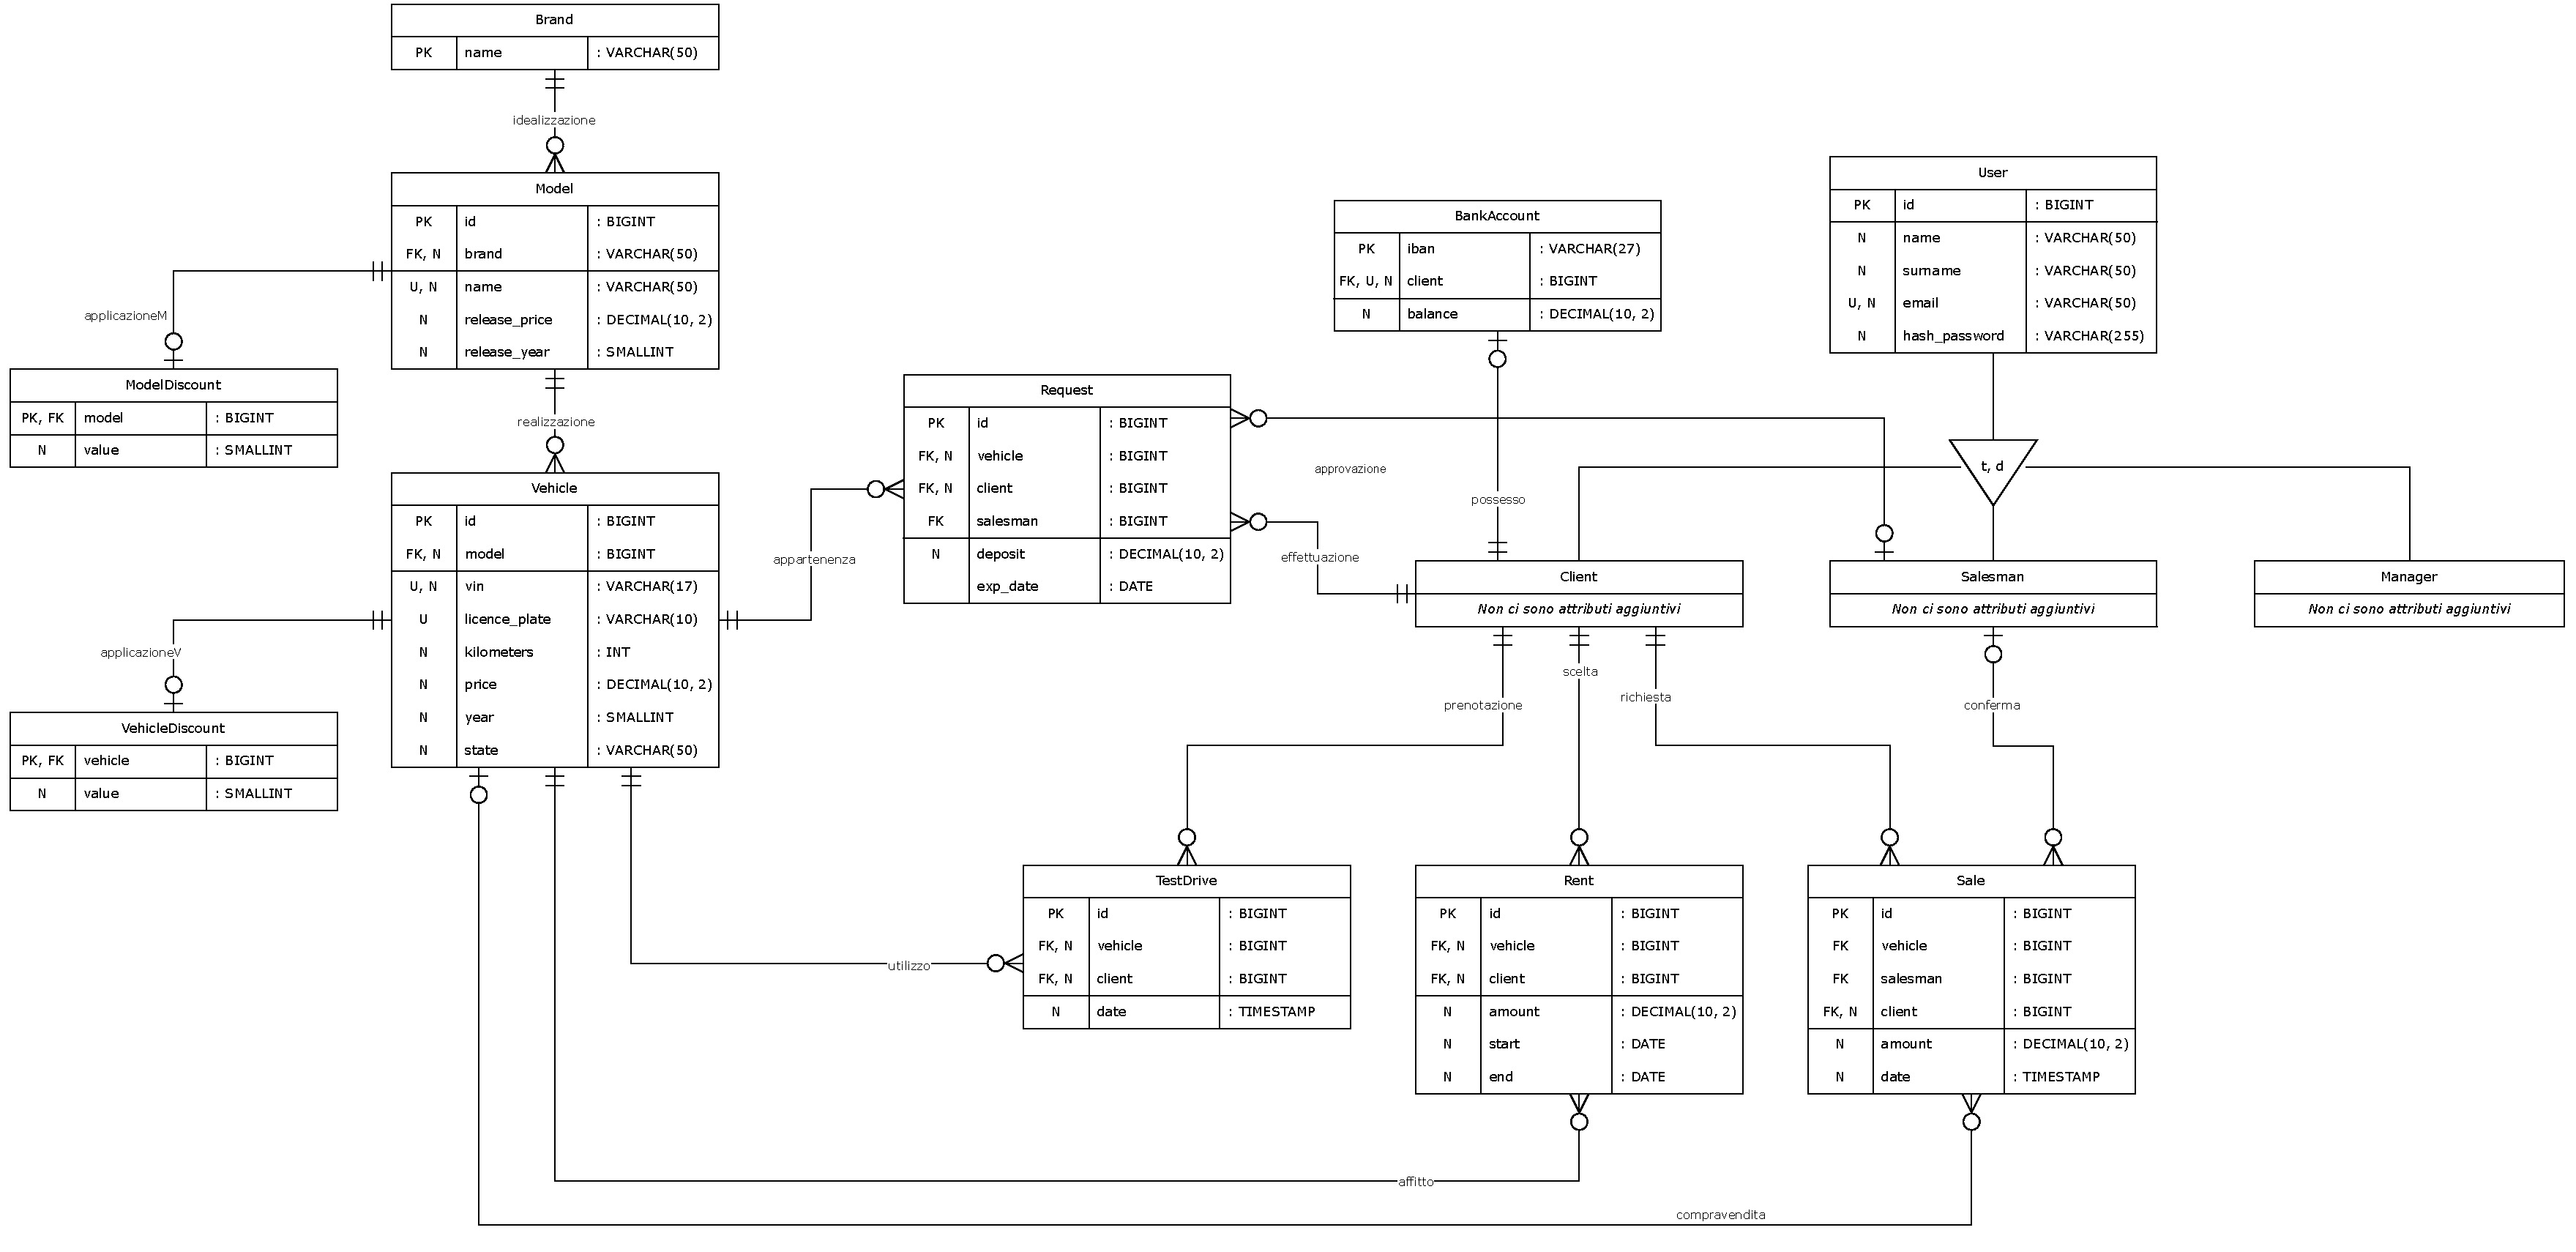
\includegraphics[width=\linewidth,height=.76\textheight,keepaspectratio]{swe-er-original.pdf}
  \caption{Schema entità--relazione di DriveHub, esportato dal diagramma originale dell'autore.}\label{fig:er-drivehub}
\end{figure}
\clearpage
DriveHub conserva catalogo, utenti e operazioni in un database relazionale. La configurazione ordinaria usa PostgreSQL tramite JDBC; la modalità dimostrativa avvia invece H2 in memoria con compatibilità PostgreSQL. Entrambe applicano \code{init.sql}, ma su H2 \code{SqlScriptRunner} omette le istruzioni procedurali specifiche di PostgreSQL, fra cui i trigger. \code{DatabaseBootstrap} registra l'applicazione dello script in \code{drivehub_schema_migrations}, così la migration non viene rieseguita a ogni avvio. Il seed dimostrativo è configurabile ed è attivo per impostazione predefinita. Il conto dei clienti è un saldo simulato nel database: non rappresenta una connessione a un istituto bancario.

La figura~\ref{fig:er-drivehub} riproduce la pagina «schema er» del file originale \texttt{docs/SWE\ ER.drawio}. I simboli alle estremità delle relazioni indicano cardinalità e partecipazione; nelle tabelle, \code{PK}, \code{FK}, \code{U} e \code{N} indicano rispettivamente chiave primaria, chiave esterna, unicità e valore non nullo. Il disegno combina la generalizzazione concettuale degli utenti con gli attributi e le chiavi delle relazioni persistenti.

\noindent\code{Brand} è associata a zero o più \code{Model}, e ciascun modello identifica zero o più \code{Vehicle}. Gli sconti di modello e veicolo sono facoltativi e al più uno per elemento. Un \code{Client} può effettuare più richieste, test drive, noleggi e compravendite. Ogni \code{Request}, \code{TestDrive} e \code{Rent} si riferisce a un cliente e a un veicolo; il \code{Salesman} di una richiesta o vendita è facoltativo. In \code{Sale} è facoltativo anche il veicolo, perché una penale viene registrata senza veicolo. Il medesimo veicolo può comparire in più vendite nel tempo, anche dopo un'acquisizione o una nuova messa in vendita. Il collegamento \code{Client}--\code{BankAccount} indica \code{1..1} sul lato \code{Client} e \code{0..1} sul lato \code{BankAccount}, in accordo con lo schema fisico: ogni conto appartiene a un cliente, mentre un cliente può avere al massimo un conto.

\subsection{Modello relazionale}\label{sec:modello-relazionale}

La traduzione delle relazioni uno-a-molti pone la chiave esterna sul lato «molti». La generalizzazione \code{User} è realizzata con tre tabelle distinte, una per ruolo, che ripetono gli attributi comuni. Lo schema fisico di \code{init.sql} comprende le tredici relazioni seguenti; la vista \code{user} non è una quattordicesima tabella.

\begin{quote}
\ttfamily\small\raggedright
brand(\uline{name})

\smallskip
model(\uline{id}, \dashuline{brand}, name, release\_price, release\_year)\\
\hspace*{2em}\textsc{unique}(name)

\smallskip
model\_discount(\uline{model}$^{\dagger}$, value)

\smallskip
vehicle(\uline{id}, \dashuline{model}, vin, licence\_plate$^{\ast}$,\\
\hspace*{2em}kilometers, price, year, state)\\
\hspace*{2em}\textsc{unique}(vin), \textsc{unique}(licence\_plate)

\smallskip
vehicle\_discount(\uline{vehicle}$^{\dagger}$, value)

\smallskip
client(\uline{id}, name, surname, email, hash\_password)\\
\hspace*{2em}\textsc{unique}(email)

\smallskip
salesman(\uline{id}, name, surname, email, hash\_password)\\
\hspace*{2em}\textsc{unique}(email)

\smallskip
manager(\uline{id}, name, surname, email, hash\_password)\\
\hspace*{2em}\textsc{unique}(email)

\smallskip
bank\_account(\uline{iban}, \dashuline{client}, balance)\\
\hspace*{2em}\textsc{unique}(client)

\smallskip
request(\uline{id}, \dashuline{vehicle}, \dashuline{client},\\
\hspace*{2em}\dashuline{salesman}$^{\ast}$, deposit, exp\_date$^{\ast}$)

\smallskip
test\_drive(\uline{id}, \dashuline{vehicle}, \dashuline{client}, date)

\smallskip
rent(\uline{id}, \dashuline{vehicle}, \dashuline{client}, amount, start, end)

\smallskip
sale(\uline{id}, \dashuline{vehicle}$^{\ast}$, \dashuline{salesman}$^{\ast}$,\\
\hspace*{2em}\dashuline{client}, amount, date)
\end{quote}

\noindent Le chiavi esterne si riferiscono alle seguenti relazioni:
\begin{quote}
\ttfamily\small\raggedright
model.brand $\rightarrow$ brand.name\\
model\_discount.model $\rightarrow$ model.id\\
vehicle.model $\rightarrow$ model.id\\
vehicle\_discount.vehicle $\rightarrow$ vehicle.id\\
bank\_account.client $\rightarrow$ client.id\\
request.vehicle, test\_drive.vehicle, rent.vehicle, sale.vehicle $\rightarrow$ vehicle.id\\
request.client, test\_drive.client, rent.client, sale.client $\rightarrow$ client.id\\
request.salesman, sale.salesman $\rightarrow$ salesman.id
\end{quote}

\begin{samepage}
\noindent\textbf{Legenda della notazione}
\begin{itemize}
\item[] \uline{attributo}: chiave primaria; \dashuline{attributo}: chiave esterna.
\item[] $^{\dagger}$: attributo che è contemporaneamente chiave primaria ed esterna.
\item[] $^{\ast}$: attributo opzionale (\code{NULL} ammesso); gli altri sono obbligatori.
\item[] \textsc{unique}(attributo): vincolo di unicità limitato alla relazione indicata.
\end{itemize}
\end{samepage}

Le date di \code{test_drive} e \code{sale} sono \code{TIMESTAMP}; \code{rent} usa \code{DATE}. Lo schema definisce inoltre \code{CHECK} su prezzi di modelli e veicoli, saldo, importo del noleggio, sconti, stato del veicolo e ordine delle date del noleggio. Non definisce un \code{CHECK} per \code{request.deposit} o \code{sale.amount}: i due campi usano anche valori negativi per distinguere operazioni diverse. Le eccezioni e i limiti di questi vincoli sono spiegati nel paragrafo seguente.

\subsection{Utenti, vincoli e semplificazioni}

Nel diagramma \code{User} raccoglie concettualmente nome, cognome, email e hash della password; \code{Client}, \code{Salesman} e \code{Manager} sono i tre ruoli. La traduzione SQL non crea una tabella \code{user}: replica gli attributi comuni nelle tre tabelle di ruolo e definisce una vista \code{user} mediante \code{UNION ALL}, aggiungendo il campo \code{role}. \code{PostgresUserDao} scrive nella tabella del ruolo e legge dalla vista quando serve una ricerca comune. Gli \code{id} sono generati separatamente nelle tre tabelle e possono quindi coincidere: per identificare un utente fra ruoli occorre considerare anche \code{role}; l'\code{id} mostrato nel supertipo non è una chiave primaria globale della vista.

La registrazione applicativa verifica che l'email non sia già utilizzata e, per un \code{Client}, crea il \code{BankAccount} nella stessa transazione. La relazione uno-a-uno mostrata nel diagramma descrive questo percorso ordinario: nel database \code{UNIQUE(client)} impedisce più conti per lo stesso cliente, ma non obbliga ogni cliente ad averne uno. Per facilitare le prove nella modalità dimostrativa, i trigger sull'email non vengono installati su H2. Su PostgreSQL \code{init.sql} definisce invece la funzione \code{check_user_email_disjoint} e tre trigger, ma il loro confronto esclude righe con lo stesso \code{id} numerico anche se provengono da tabelle diverse. Gli ID dei ruoli sono indipendenti, quindi i trigger non assicurano l'unicità trasversale in tutti i casi. \code{UNIQUE(email)} vale all'interno di ciascuna tabella; il normale percorso di registrazione esegue anche una ricerca preventiva nella vista \code{user}.

Le regole espresse nello schema includono, fra le altre, \code{UNIQUE} su VIN e targa, saldo non negativo, sconti fra 0 e 50, stato del veicolo limitato a \code{WAITING}, \code{SALE}, \code{RENT}, \code{BLOCKED} e \code{SOLD}, e fine del noleggio non precedente all'inizio. Altre condizioni restano applicative: non esiste un vincolo SQL che impedisca la sovrapposizione temporale di due \code{Rent} o renda unico lo slot di \code{TestDrive}. Il segno di \code{Request.deposit} distingue l'acconto d'acquisto dalla stima di cessione; il segno di \code{Sale.amount} distingue la vendita dall'esborso per un'auto acquisita. Una penale è una \code{Sale} con \code{vehicle} e \code{salesman} nulli. Lo schema consente queste rappresentazioni, ma non contiene \code{CHECK} che ne garantiscano tutte le combinazioni ammissibili.


\chapter{Implementazione}\label{ch:implementazione}
Questo capitolo descrive le scelte implementative dei livelli \code{domain}, \code{business}, \code{presentation} e \code{dao}, concentrandosi sulle classi e sulle regole che guidano i casi d'uso principali. Gli esempi di codice provengono dai sorgenti di DriveHub; i diagrammi del capitolo precedente ne mostrano le relazioni.

\section{Domain Model}\label{sec:implementazione-dominio}

Il Domain Model rappresenta veicoli, utenti e operazioni senza importare classi di \code{presentation}, \code{business} o \code{dao}. È organizzato in cinque pacchetti, già mostrati nel diagramma di classe della figura~\ref{fig:classi-domain}:
\begin{itemize}
  \item \textbf{users}: identità, ruolo e conto dimostrativo del cliente;
  \item \textbf{vehicles}: catalogo, stato dei veicoli e sconti;
  \item \textbf{rentals}: noleggi e prenotazioni di test drive;
  \item \textbf{sales}: richieste, compravendite e penali;
  \item \textbf{observer}: contratti ed eventi relativi all'inventario.
\end{itemize}
Alla radice di \code{domain}, \code{BaseEntity} conserva l'ID delle entità persistite. Una nuova entità nasce con ID nullo; \code{assignId} accetta soltanto valori positivi e impedisce di sostituire un ID già assegnato con uno diverso. \code{requireId} segnala invece l'uso di un'entità ancora priva di identità persistente. Le associazioni fra gli oggetti sono rappresentate soprattutto da ID: per esempio \code{Vehicle} conserva \code{modelId} e \code{Request} conserva \code{vehicleId} e \code{clientId}. Il caricamento degli oggetti associati spetta ai DAO e ai servizi.

\subsection{Users}
Il pacchetto \code{users} contiene \code{User}, \code{Role} e \code{BankAccount}. A differenza della gerarchia concettuale nello schema ER, nel codice Java \code{Client}, \code{Salesman} e \code{Manager} non sono sottoclassi: sono valori del campo \code{role} di un'unica classe \code{User}. L'enumerazione contiene \code{CLIENT}, \code{CUSTOMER}, \code{SALESMAN} e \code{MANAGER}; \code{Role.fromString} converte il vecchio nome \code{CUSTOMER} in \code{CLIENT}. La persistenza dei ruoli in tabelle distinte è descritta nel paragrafo~\ref{sec:dati}.

Il costruttore di \code{User} richiede nome, cognome e hash non vuoti; normalizza l'email in minuscolo e ne controlla il formato. La factory \code{create} produce un utente senza ID, che il DAO assegna dopo l'inserimento. Il controllo di unicità dell'email richiede una ricerca nei dati persistiti: il singolo oggetto non può garantirlo. \code{equals} e \code{hashCode} si basano sull'email, indipendentemente dal ruolo; questa scelta presuppone che il normale flusso applicativo eviti email duplicate fra ruoli.

\code{BankAccount} non deriva da \code{BaseEntity}: è identificato dall'IBAN e conserva l'ID del cliente intestatario. Il costruttore richiede un IBAN di 27 caratteri e un saldo non negativo. I metodi \code{deposit} e \code{withdraw} ammettono solo importi positivi; il prelievo verifica anche che il saldo sia sufficiente prima di aggiornarlo. Il conto rappresenta un saldo simulato, senza collegamento a un servizio bancario esterno.

\subsection{Vehicles}
Il pacchetto \code{vehicles} riunisce \code{Brand}, \code{VehicleModel}, \code{Vehicle}, \code{VehicleState}, \code{ModelDiscount} e \code{VehicleDiscount}. \code{Brand} richiede un nome non vuoto; \code{VehicleModel} associa marca, nome, prezzo e anno di lancio, rifiutando prezzi negativi e anni fuori dall'intervallo 1900--anno corrente. Gli sconti di modello e di veicolo sono percentuali intere fra 0 e 50 e conservano l'ID del rispettivo elemento.

\code{Vehicle} conserva il modello, il VIN, l'eventuale targa, chilometraggio, prezzo, anno e stato. Il costruttore normalizza VIN e targa in maiuscolo, rifiuta chilometri e prezzi negativi e impone chilometri zero quando la targa manca. \code{VehicleState} comprende \code{WAITING}, \code{SALE}, \code{RENT}, \code{BLOCKED} e \code{SOLD}. Tre metodi esprimono transizioni con una precondizione esplicita:
\begin{lstlisting}[language=Java,caption={Transizioni controllate dello stato di Vehicle.}]
public void approve() {
    if (state != VehicleState.WAITING) {
        throw new DomainRuleViolationException(
                "Cannot approve vehicle not in WAITING state");
    }
    this.state = VehicleState.SALE;
}

public void block() {
    if (state != VehicleState.SALE) {
        throw new DomainRuleViolationException(
                "Cannot block vehicle not in SALE state");
    }
    this.state = VehicleState.BLOCKED;
}
\end{lstlisting}
\code{unblock} applica la stessa struttura al passaggio da \code{BLOCKED} a \code{SALE}. Esiste anche \code{transitionTo}, che assegna qualsiasi \code{VehicleState} non nullo, e \code{updateDetails} riceve direttamente il nuovo stato: dunque la classe non impone a ogni chiamante l'uso delle tre transizioni controllate. I servizi devono verificare il contesto dell'operazione; il database limita i valori ammessi, ma non l'ordine dei passaggi.

\subsection{Rentals}
\code{Rent} e \code{TestDrive} condividono il riferimento a un cliente e a un veicolo, ma modellano tempi diversi. \code{Rent} registra un intervallo di giorni \code{LocalDate} e un importo non negativo; il costruttore respinge una data finale precedente a quella iniziale. \code{TestDrive} registra invece un \code{LocalDateTime} e verifica che l'ora di partenza sia fra le 09:00 e le 16:00 con minuti pari a zero. Il metodo \code{end} restituisce l'ora successiva alla partenza.

Nessuna delle due classi contiene uno stato di workflow. Un oggetto \code{Rent} valido può comunque sovrapporsi a un altro noleggio dello stesso veicolo, e due oggetti \code{TestDrive} validi possono avere lo stesso slot: sono verifiche che richiedono la consultazione delle prenotazioni già registrate. I servizi eseguono queste ricerche prima del salvataggio; il rischio residuo delle richieste concorrenti è discusso nella sezione~\ref{sec:concorrenza}.

\subsection{Sales}
Il pacchetto \code{sales} contiene \code{Request} e \code{Sale}. \code{Request} rappresenta due pratiche con lo stesso insieme di campi. \code{createPurchase} richiede un acconto positivo per l'acquisto dal catalogo; \code{createSaleProposal} richiede una stima positiva e la salva con segno negativo per la proposta di cessione del cliente:
\begin{lstlisting}[language=Java,caption={Factory method di Request per i due tipi di pratica.},label={lst:request}]
public static Request createPurchase(long vehicleId, long clientId,
                                     BigDecimal deposit) {
    if (deposit.compareTo(BigDecimal.ZERO) <= 0) {
        throw new IllegalArgumentException(
                "Purchase deposit must be strictly positive");
    }
    return new Request(null, vehicleId, clientId, null, deposit, null);
}

public static Request createSaleProposal(long vehicleId, long clientId,
                                         BigDecimal estimatedValue) {
    if (estimatedValue.compareTo(BigDecimal.ZERO) <= 0) {
        throw new IllegalArgumentException(
                "Estimated value must be strictly positive");
    }
    return new Request(null, vehicleId, clientId, null,
                       estimatedValue.negate(), null);
}
\end{lstlisting}
Il costruttore vieta un valore zero e \code{isPurchase}/\code{isSaleProposal} distinguono le due pratiche dal segno. L'eventuale \code{salesmanId} e la scadenza sono assegnati in un momento successivo tramite i metodi della richiesta. La codifica compatta evita due tipi persistenti separati, ma rende necessario interpretare correttamente il segno nei servizi e nelle query.

\code{Sale} è il registro degli esiti economici. Un importo positivo con veicolo rappresenta una vendita al cliente; un importo negativo rappresenta l'acquisizione di un'auto dal cliente. La factory \code{penalty} costruisce una riga senza veicolo né venditore per la penale. \code{isAcquisition} controlla il segno e \code{isPenalty} controlla i due riferimenti nulli. Il costruttore, però, richiede soltanto cliente positivo, importo e data non nulli: non impedisce ogni combinazione incoerente di segno e riferimenti. La coerenza del caso d'uso resta responsabilità dei servizi.

\subsection{Observer}
Il pacchetto \code{observer} definisce \code{InventorySubject}, \code{InventoryObserver}, il record \code{InventoryEvent} e l'enumerazione \code{InventoryEventType}. L'evento trasporta tipo, veicolo interessato, targa, eventuale stato precedente e successivo, e istante di creazione. Le factory \code{statusChanged} e \code{requestExpired} preparano i dati degli eventi più ricorrenti.

Le interfacce appartengono al dominio, mentre i soggetti concreti sono \code{SalesService} e \code{RentalService} nel livello business. Questi servizi registrano gli observer e li notificano quando un'operazione modifica l'inventario. Il record descrive il fatto avvenuto, senza conoscere controller o database; la notifica, tuttavia, è eseguita dal servizio durante l'operazione e non costituisce una garanzia di consegna dopo il commit della transazione.

\section{Business Layer}\label{sec:business-layer}

Il Business Layer coordina le entità del dominio per eseguire i casi d'uso. I servizi ottengono i dati attraverso le interfacce DAO e delegano alle entità le regole che queste possono verificare autonomamente. Il diagramma della figura~\ref{fig:classi-business} mostra le dipendenze principali. Il package \code{business} è suddiviso in sei parti:
\begin{itemize}
  \item \textbf{services}: servizi applicativi per identità, catalogo, conto, test drive, noleggio, vendita e prezzi; contiene anche \code{RegistrationRequest} e \code{CatalogModels};
  \item \textbf{core}: \code{TransactionRunner}, che esegue un lavoro all'interno di una \code{UnitOfWork};
  \item \textbf{strategies}: algoritmi sostituibili per prezzi, noleggi e valutazioni;
  \item \textbf{security}: contratto \code{PasswordHasher} e implementazione \code{Pbkdf2PasswordHasher};
  \item \textbf{banking}: \code{IbanGenerator} per il conto simulato del cliente;
  \item \textbf{exceptions}: errori applicativi per autenticazione, conflitti e risorse assenti.
\end{itemize}
La separazione mantiene le query nelle porte DAO, la verifica del saldo in \code{BankAccount} e la scelta del flusso nei servizi. Il business dipende dal dominio e dalle interfacce di persistenza, non dai controller JavaFX né dalle classi JDBC concrete.

\subsection{Core: unità di lavoro e transazioni}
Ogni servizio costruisce un \code{TransactionRunner} a partire da \code{DaoFactory}. \code{execute} apre un'unità di lavoro, passa la stessa istanza alla lambda del caso d'uso, esegue il commit se il lavoro termina e il rollback se viene lanciata un'eccezione. Il \code{try}-with-resources chiude l'unità anche in caso di errore:
\par\medskip\noindent\begin{minipage}{\linewidth}
\begin{lstlisting}[language=Java,caption={Nucleo di TransactionRunner.execute, dal sorgente corrente.},label={lst:transaction-runner}]
try (UnitOfWork unit = daoFactory.begin()) {
    try {
        T result = work.apply(unit);
        unit.commit();
        return result;
    } catch (RuntimeException | Error failure) {
        try {
            unit.rollback();
        } catch (RuntimeException rollbackFailure) {
            failure.addSuppressed(rollbackFailure);
        }
        throw failure;
    }
}
\end{lstlisting}
\end{minipage}\par\medskip
Questo meccanismo lega fra loro le scritture eseguite nella stessa lambda, come saldo e registrazione di un noleggio. Non unifica però due chiamate di servizio separate; inoltre una chiamata annidata a \code{execute} apre un'altra \code{UnitOfWork}. L'implementazione JDBC del contratto è descritta nella sezione~\ref{sec:transazioni}.

\subsection{Services: responsabilità}
\code{AuthService} gestisce registrazione, login e modifiche dell'account; \code{BankAccountService} consulta e aggiorna il saldo del cliente. \code{CatalogService} legge e modifica marche, modelli e veicoli. \code{TestDriveService} e \code{RentalService} verificano disponibilità temporali e salvano le prenotazioni. \code{SalesService} governa richieste di acquisto, saldo, penali e proposte di cessione. \code{PricingService} legge modello e sconti e passa i dati alla strategia di prezzo. La classe di supporto \code{CatalogModels} trova o crea marca e modello durante la proposta di un veicolo; \code{RegistrationRequest} trasporta i dati necessari alla registrazione.

La distinzione fra validazione locale e verifica applicativa è visibile nel test drive. \code{TestDrive} valida l'ora contenuta nel proprio oggetto; \code{TestDriveService.book} deve anche interrogare le prenotazioni già presenti, il noleggio del veicolo e il numero di test drive attivi del cliente. Analogamente \code{Rent} valida date e importo, mentre \code{RentalService.bookRental} decide disponibilità, prezzo e addebito. I paragrafi seguenti esaminano questi flussi e le altre decisioni dei servizi.

\subsection{Services: flussi applicativi}\label{sec:flussi-implementati}
I servizi coordinano le porte DAO entro \code{TransactionRunner.execute}. Le tre sequenze della sezione~\ref{sec:sequenze} visualizzano le chiamate principali; qui sono analizzate le decisioni e le scritture, incluse le alternative che un diagramma compatto non rende leggibili.

\subsubsection{Catalogo e test drive}
\code{CatalogService.availableForSale}, \code{availableForRental} e \code{waitingVehicles} interrogano \code{VehicleDao.findByState}. \code{ServiceUiGateway.searchCatalog} applica poi in memoria un testo a descrizione, VIN e targa e calcola il prezzo esposto con \code{PricingService.quotePrice}. Il filtro viene quindi eseguito in parte dal database e in parte dal gateway. La UI non offre il prezzo massimo promesso da \code{RF-CAT-01}.

\code{TestDriveService.book} controlla prima data e ora, poi carica il veicolo. Ammette \code{SALE} e \code{RENT}; limita a tre i test drive attivi del cliente; interroga \code{RentalDao.isVehicleRentedOnDate} e \code{TestDriveDao.hasConflictingTestDrive}; infine salva \code{TestDrive}. Lo slot applicativo è un'ora, con partenza alle 09:00--16:00. Il servizio tronca i minuti della \code{LocalTime} al costruire \code{dateTime}, quindi un input con minuti diversi da zero viene ricondotto all'inizio dell'ora anziché rifiutato in quel punto. Il costruttore \code{TestDrive} ammette solo minuti zero.

\par\medskip\noindent\begin{minipage}{\linewidth}
\begin{lstlisting}[language=Java,caption={Controlli sequenziali di disponibilità nel test drive, estratto da \code{TestDriveService.book}.},label={lst:test-drive-book}]
if (unit.rentals().isVehicleRentedOnDate(vehicleId, date)) {
    throw new ConflictException("Il veicolo e noleggiato per il giorno selezionato");
}
if (unit.testDrives().hasConflictingTestDrive(vehicleId, dateTime)) {
    throw new ConflictException("La fascia oraria e gia occupata");
}
TestDrive testDrive = TestDrive.create(vehicleId, clientId, dateTime);
return unit.testDrives().save(testDrive);
\end{lstlisting}
\end{minipage}\par\medskip
Nel listato le stringhe di errore sono abbreviate per mostrare le chiamate rilevanti; per i messaggi letterali si rimanda al sorgente. Le due letture non bloccano un inserimento concorrente: l'assenza di una unique su \code{(vehicle,date)} è discussa in sezione~\ref{sec:concorrenza}.

\subsubsection{Noleggio con saldo del conto}
La UI mostra un preventivo per \code{days = DAYS.between(start,end)+1}. Alla conferma, \code{RentalService.bookRental} ripete i controlli e ricalcola l'importo. L'algoritmo verifica stato \code{RENT} e overlap, poi trova il conto del cliente, esegue \code{BankAccount.withdraw}, salva il nuovo saldo, inserisce \code{Rent} e cancella test drive nel periodo. Tutte le scritture DAO passano sulla stessa \code{PostgresUnitOfWork}. Non esiste un pagamento con stato \code{PENDING}/\code{COMPLETED}/\code{FAILED}: \code{RF-PAY-01} è quindi coperto soltanto dall'addebito dimostrativo.

La query di overlap usa gli estremi inclusivi. Per prenotazioni già salvate dello stesso veicolo, \code{NOT ("end" < ? OR start > ?)} rileva un'intersezione. Due periodi adiacenti che condividono un giorno sono conflittuali; uno che inizia il giorno dopo la fine dell'altro è ammesso. Lo schema protegge \code{end >= start} ma non l'assenza di sovrapposizioni, perciò il controllo non è sicuro sotto concorrenza.
\begin{lstlisting}[language=SQL,caption={Predicato di overlap da \code{PostgresRentalDao.hasOverlappingRentals}.},label={lst:overlap}]
SELECT 1 FROM "rent"
WHERE vehicle = ? AND NOT ("end" < ? OR start > ?)
LIMIT 1
\end{lstlisting}

\code{RentalService.switchVehicleState} è un secondo flusso significativo. Quando un Salesman passa un veicolo da \code{RENT} a \code{SALE}, il servizio legge noleggi futuri, riaccredita l'intero importo sui conti dei clienti e cancella le righe \code{rent}; quindi cambia lo stato del veicolo. L'operazione è in una transazione JDBC, ma le notifiche Observer vengono emesse durante l'esecuzione della lambda, prima del commit. Nel verso \code{SALE} a \code{RENT} il codice non compie il medesimo rimborso.

\subsubsection{Richiesta di acquisto, saldo e penale}
Il controller calcola l'acconto come 20\% di \code{selectedCatalogVehicle.price()} e chiede conferma. \code{SalesService.requestPurchase} riceve però l'importo dal chiamante senza confrontarlo con \code{PricingStrategy.calculateDeposit}: un client alternativo può passare un valore positivo diverso. Il metodo controlla \code{VehicleState.SALE}, sottrae l'acconto dal conto, aggiorna il veicolo a \code{BLOCKED} e salva \code{Request.createPurchase}. \code{authorizePurchase} aggiunge \code{salesmanId} e \code{expDate = LocalDate.now().plusMonths(1)}.

\code{CustomerWorkspaceController.payFullBalance} nasconde il comando finché \code{expDate} è nulla; il controllo però non è ripetuto in \code{SalesService.completePurchase}. Quest'ultimo calcola \code{remaining = vehicle.price() - request.deposit()}, preleva il residuo se positivo, imposta \code{SOLD}, elimina la richiesta, salva \code{Sale} e cancella i futuri test drive. Il prezzo di partenza del saldo è il campo \code{Vehicle.price}, mentre il catalogo mostra \code{PricingService.quotePrice}; lo sconto mostrato non è conservato nella \code{Request}. La differenza va risolta come regola commerciale, senza supporre che i due importi coincidano sempre.

Se una richiesta scade o viene annullata, \code{cancelRequestWithPenalty} calcola una penale del 20\% dell'acconto con \code{HALF_UP}, rimborsa il restante 80\%, cancella la richiesta, riporta il veicolo in \code{SALE} e salva una \code{Sale.penalty}. \code{processExpiredRequests} ricerca le pratiche scadute e chiama quel metodo separatamente per ognuna; cattura e ignora le eccezioni della singola pratica. L'elaborazione avviene all'accesso e in alcune letture del gateway, non tramite scheduler persistente.

\subsubsection{Proposta di cessione del veicolo}
\code{SalesService.submitVehicleForSale} usa \code{CatalogModels.findOrCreate} per marca e modello, quindi \code{PricingService.calculateValuation}. Un VIN già presente è ammesso soltanto se il veicolo precedente è \code{SOLD}; in quel caso la riga viene aggiornata a \code{WAITING}, altrimenti viene creata una nuova riga. \code{Request.createSaleProposal} memorizza il valore stimato con segno negativo. La proposta non attraversa un'offerta modificabile dal Salesman e una successiva approvazione Manager come nella specifica storica.

\code{approveClientSale} porta il veicolo a \code{SALE}, accredita al cliente il valore assoluto della \code{Request}, registra una \code{Sale} negativa ed elimina la richiesta. \code{rejectClientSale} elimina la richiesta e conserva il veicolo come \code{SOLD} solo se esistono vendite pregresse, altrimenti lo elimina. Quando trova la proposta, il controller del Salesman chiama direttamente \code{approveClientSale} passando l'ID della sessione; usa \code{approveVehicle} se non trova alcuna proposta per il veicolo selezionato. Se \code{approveVehicle} viene chiamato direttamente su una proposta, chiama \code{approveClientSale} all'interno di un'altra lambda transazionale, aprendo una seconda unità di lavoro, e passa il valore costante \code{1L} come ID del Salesman. Questa scorciatoia può attribuire la vendita al venditore sbagliato quando opera un altro account. Il confine annidato è analizzato in sezione~\ref{sec:transazioni}.

La stima esposta prima della proposta può divergere dal valore poi salvato: \code{quoteValuation} usa un prezzo di rilascio predefinito di 25.000 quando non trova il modello, mentre \code{CatalogModels.findOrCreate} usa l'importo fornito o 20.000 per creare il nuovo modello. Sono due fallback diversi nei sorgenti, non una policy documentata da un requisito.

\subsection{Strategies: prezzi e sconti}\label{sec:pricing}
\code{PricingService} dipende da \code{PricingStrategy}; la composizione normale istanzia \code{StandardPricingStrategy}. La porta rende sostituibile l'algoritmo nei test o in una futura revisione. La persistenza offre al massimo uno sconto per modello e uno per veicolo; \code{quotePrice} sceglie il maggiore fra i due valori, non li cumula. \code{ModelDiscount} e \code{VehicleDiscount} ammettono interi fra 0 e 50, coerenti con i CHECK SQL.

Per un veicolo in catalogo, la strategia parte da \code{VehicleModel.releasePrice}; se la targa non è nulla applica un fattore $0{,}80$, poi $1-p/100$ con $p$ pari allo sconto promozionale maggiore, quindi $0{,}95^{a}$ per gli anni trascorsi e $0{,}95^{\lfloor km/10000\rfloor}$ per il chilometraggio. Il risultato è arrotondato a due decimali con \code{HALF_UP} e non scende sotto zero. La formula è una scelta del codice e non va confusa con un prezzo di mercato verificato:
\[
P_{\mathrm{catalogo}}=
\operatorname{round}_{2}\!\left(
P_{\mathrm{lancio}}\cdot f_{\mathrm{targa}}
\cdot (1-p/100)\cdot 0{,}95^{a+\lfloor km/10000\rfloor}
\right),\qquad
f_{\mathrm{targa}}\in\{1;0{,}80\}.
\]
\code{calculateDeposit(price)} restituisce il 20\% del prezzo passato dal chiamante. Nel flusso GUI l'acconto è calcolato sul prezzo mostrato; \code{SalesService.requestPurchase}, tuttavia, non ricontrolla la percentuale.

Per rendere verificabile la distinzione fra prezzi, si consideri un esempio ipotetico coerente con il codice: modello e \code{Vehicle.price} a 40.000 euro, veicolo nuovo senza targa e promozione del 10\%. \code{quotePrice} mostra 36.000 euro e la UI calcola un acconto di 7.200 euro. Il metodo \code{completePurchase} sottrae invece tale acconto da \code{Vehicle.price} e chiede 32.800 euro; l'esborso totale diventa 40.000 euro. L'esempio non afferma che una transazione del dataset abbia questi valori: mostra perché è necessario fissare il prezzo preventivato nella pratica o ricalcolare il saldo con una regola esplicita.

Il noleggio usa \code{Vehicle.price}, non \code{quotePrice}. Per $d$ giorni inclusivi, \code{rentalPrice} calcola una tariffa base giornaliera di $\mathrm{price}/1000$, poi un fattore $0{,}95^{d-1}$ sul totale; arrotonda a centesimi e impone un minimo di 0,01. La label della UI in \code{CustomerWorkspaceController.updateRentalQuotePreview} dice invece «Sconto 5\% ogni 5 gg applicato»: il testo non corrisponde alla formula corrente e deve essere corretto o accompagnato da una modifica della policy. La valutazione del veicolo ceduto riusa il fattore targa, età e km, senza promozione Manager.

\begin{longtable}{p{.25\linewidth}p{.39\linewidth}p{.28\linewidth}}
\caption{Origine degli importi nei flussi economici.}\label{tab:prezzi}\\
\toprule Importo & Origine nel codice & Uso\\\midrule\endfirsthead
\toprule Importo & Origine nel codice & Uso\\\midrule\endhead
Prezzo esposto nel catalogo & \code{PricingService.quotePrice} & Anteprima di acquisto\\
Acconto GUI & 20\% di \code{VehicleItem.price} & \code{requestPurchase}\\
Saldo effettivo & \code{Vehicle.price - Request.deposit} & \code{completePurchase}\\
Prezzo noleggio & \code{StandardPricingStrategy.rentalPrice} & \code{bookRental}\\
Stima cessione & \code{calculateValuation} & \code{submitVehicleForSale}\\
\bottomrule
\end{longtable}

\subsection{Security e Banking: autenticazione e conto}\label{sec:sicurezza}
\code{AuthService.register} normalizza l'email, ne verifica l'assenza tramite \code{UserDao.findByEmail}, calcola l'hash e salva \code{User}. Se il ruolo è \code{CLIENT} o \code{CUSTOMER}, crea nello stesso \code{UnitOfWork} un \code{BankAccount} con saldo iniziale zero e IBAN derivato da \code{IbanGenerator}. \code{login} cerca l'email e chiama \code{PasswordHasher.verify}. Il verificatore \code{Pbkdf2PasswordHasher} usa PBKDF2-HMAC-SHA256, sale casuale di 16 byte, 210.000 iterazioni e chiave di 256 bit nei parametri predefiniti; confronta l'hash con \code{MessageDigest.isEqual}. La password non è salvata in chiaro.

Il conto dimostrativo mantiene l'invariante del saldo in \code{BankAccount.withdraw}: un importo nullo o non positivo è rifiutato; se il saldo è inferiore all'importo il metodo lancia \code{DomainRuleViolationException}; solo dopo aggiorna il valore in memoria. Le varianti per IBAN di deposito e prelievo in \code{BankAccountService} recuperano il conto con \code{findByIbanForUpdate}; le varianti per ID cliente e i flussi di noleggio e vendita usano \code{findByClientId}, senza quel lock. Questa distinzione è rilevante sotto concorrenza: la presenza di un lock in un percorso non lo estende agli altri.

Nella UI, \code{RegistrationController} converte il campo password in \code{char[]} e lo azzera dopo la richiesta. La route successiva dipende dal ruolo restituito. \code{AuthService.updateEmail}, \code{updatePassword} e \code{deleteAccount} richiedono la password corrente; l'eliminazione è rifiutata se il DAO trova operazioni collegate. Tali controlli non eliminano le lacune seguenti, che vanno tenute separate dalla proprietà dell'hash:
\begin{itemize}
\item \code{RegistrationController} espone pubblicamente anche \code{SALESMAN} e \code{MANAGER}; è una scelta da prototipo, non provisioning sicuro dello staff.
\item \code{DatabaseConfig} offre una password DB di fallback e seed demo attivo per default, in contrasto con \code{README.md}. I valori devono essere scelti esplicitamente prima di un'installazione non dimostrativa.
\item Il guard \code{Route.allows} protegge la navigazione, mentre i servizi ricevono ID da parametri e non verificano il ruolo o la proprietà di ogni operazione. \code{ServiceUiGateway.completePurchase} ignora il \code{clientId} ricevuto nel controllo del proprietario della \code{Request}.
\item \code{AbstractController.showError} mostra \code{Throwable.getMessage()}. Le eccezioni dei DAO o dei servizi potrebbero quindi rivelare dettagli oltre a un messaggio d'uso; manca una traduzione centralizzata degli errori.
\end{itemize}

\subsection{Observer e gestione dell'inventario}\label{sec:observer}
\code{SalesService} e \code{RentalService} implementano \code{InventorySubject}. Gli observer sono conservati in una \code{CopyOnWriteArrayList}. \code{InventoryEvent} trasporta tipo, ID e targa del veicolo, stato precedente/corrente e istante. Il codice produce, fra gli altri, \code{STATUS_CHANGED}, \code{REQUEST_EXPIRED}, \code{TEST_DRIVES_CANCELLED_VEHICLE_UNAVAILABLE} e \code{RENTALS_CANCELLED_STATE_CHANGE}. Il literal \code{STOCK_RECEIVED} nell'enum non prova l'esistenza di un modulo stock, assente dai sorgenti correnti.

La notifica agli observer avviene durante la transazione del servizio, prima del commit. L'handler cattura eccezioni dei subscriber e continua. Queste due scelte impediscono all'Observer di far fallire una vendita per errore di un listener, ma un rollback successivo può lasciare un evento già osservato per una modifica non persistita. La garanzia after-commit dichiarata in \code{docs/ARCHITETTURA_E_DATI.md} appartiene alla baseline storica, non a questa implementazione.

\section{Presentation Layer}\label{sec:implementazione-ui}
Il livello di presentazione collega le viste JavaFX ai casi d'uso del Business Layer. Le schermate sono definite nei file FXML; i controller leggono gli input, invocano \code{UiGateway} e aggiornano i controlli grafici con i record di \code{UiModels}. Non costruiscono DAO né connessioni JDBC. DriveHub raccoglie le funzioni di ciascun ruolo in un workspace con più schede. Il diagramma delle classi della figura~\ref{fig:classi-presentation} mostra i componenti e le loro dipendenze.

\subsection{Controller e aree applicative}
I sei controller corrispondono alle tre pagine pubbliche e ai tre workspace autenticati:
\begin{itemize}
  \item \textbf{WelcomeController}: apre login e registrazione;
  \item \textbf{LoginController}: invia le credenziali al gateway, apre la sessione e passa al workspace del ruolo autenticato;
  \item \textbf{RegistrationController}: raccoglie anagrafica, credenziali e ruolo, registra l'utente e apre la sessione;
  \item \textbf{CustomerWorkspaceController}: gestisce catalogo, richieste di acquisto, saldo finale, noleggi, test drive, proposta di cessione, conto dimostrativo e profilo;
  \item \textbf{SalesmanWorkspaceController}: mostra veicoli e richieste in attesa, approva o rifiuta le proposte, autorizza gli acquisti e cambia la destinazione dei veicoli tra vendita e noleggio;
  \item \textbf{ManagerWorkspaceController}: gestisce marche, modelli, veicoli e sconti e consulta l'elenco delle vendite.
\end{itemize}
\code{AbstractController}, ereditato da tutti salvo \code{WelcomeController}, centralizza l'accesso al gateway e alla sessione, la conversione degli input numerici e la visualizzazione di messaggi di successo o errore. I controller restano responsabili anche di alcune verifiche utili all'interazione, come la presenza di una selezione e l'abilitazione delle date nei calendari. Molti controlli di stato vengono ripetuti dai servizi, ma non tutte le verifiche della UI lo sono: il saldo dell'acquisto, per esempio, non ricontrolla nel servizio autorizzazione, scadenza e identità del cliente.

\subsection{Creazione dei controller e navigazione}
\code{DriveHubApplication.start} costruisce il gateway, lo inserisce in \code{ApplicationContext} e inizializza \code{NavigationManager}. Quando viene aperta una route, \code{FXMLLoader} crea il controller e inietta i campi \code{@FXML}; subito dopo \code{NavigationManager.show} gli passa il contesto, se implementa \code{ContextAware}. L'ordine è rilevante: \code{initialize()} prepara i controlli, mentre \code{onContextReady()} può interrogare il gateway e popolare la vista. Nei workspace, quest'ultimo metodo richiama \code{refresh()} dopo aver ricevuto il contesto.

\begin{lstlisting}[language=Java,caption={Passaggio del contesto dopo il caricamento della vista.},label={lst:context-aware}]
FXMLLoader loader = new FXMLLoader(resource);
Parent root = loader.load();
Object controller = loader.getController();
if (controller instanceof ContextAware aware) {
    aware.setApplicationContext(context);
}
\end{lstlisting}

La classe \code{Route} associa a ogni vista il file FXML e l'insieme dei ruoli ammessi. \code{NavigationManager.show} controlla la sessione prima di caricare una route privata; \code{showHomeForCurrentRole} apre il workspace di Customer, Salesman o Manager; \code{logout} svuota la sessione e torna a \code{WELCOME}. Il controllo della route protegge la navigazione, ma non sostituisce l'autorizzazione delle singole operazioni. In particolare, \code{ServiceUiGateway.completePurchase} riceve gli identificatori del cliente e della richiesta e delega al servizio senza confrontarli con la sessione: il requisito \code{RNF-SEC-02} non è quindi garantito universalmente dal solo Presentation Layer.

\subsection{Gateway, dati della UI e aggiornamento}
\code{UiGateway} è il contratto consumato dai controller; \code{ServiceUiGateway} lo implementa usando i servizi applicativi. Le query come \code{searchCatalog}, \code{clientRentals} e \code{allSales} restituiscono record di \code{UiModels}, adatti alle tabelle JavaFX. I comandi come \code{bookRental}, \code{bookTestDrive} e \code{requestPurchase} sono invece \code{void}: dopo un esito positivo il controller richiama \code{refresh()} e rilegge i dati. Questo evita di considerare la copia mostrata nella tabella come stato aggiornato del database.

Nel workspace del cliente, ad esempio, \code{refresh()} usa l'identificatore della sessione per ricaricare richieste, vendite, noleggi e test drive; aggiorna poi il conto tramite \code{getBankAccount}. I workspace del venditore e del manager ricaricano analogamente le rispettive liste dopo le operazioni. \code{SessionContext} conserva solo la sessione corrente, mentre saldo, catalogo e pratiche sono letti dal gateway. Un preventivo di noleggio viene mostrato prima della conferma, ma \code{RentalService.bookRental} ricalcola l'importo quando esegue il caso d'uso: il valore a schermo non è il vincolo di prezzo.

La registrazione espone nella \code{ComboBox} anche i ruoli Salesman e Manager, oltre a Client. È una scelta presente nell'interfaccia corrente; in un sistema distribuito l'assegnazione dei ruoli privilegiati richiederebbe un percorso amministrato. Anche per questo le guardie di navigazione e i controlli dei controller vanno letti come comportamento della UI, non come prova di autorizzazione end-to-end.

\section{Persistenza: livello DAO e mapping oggetti/tabelle}\label{sec:persistenza}\label{sec:dao}
Il livello DAO traduce oggetti del dominio e righe SQL senza ricorrere a un ORM. Le query e il mapping sono scritti in JDBC, con \code{PreparedStatement} per i parametri. Le interfacce del package \code{dao.interfaces} costituiscono le porte usate dai servizi; le classi \code{dao.postgres} ne forniscono le implementazioni. Il diagramma della figura~\ref{fig:classi-dao} mostra factory, unità di lavoro e DAO rappresentativi.

\subsection{Porte DAO e implementazioni JDBC}
DriveHub definisce una porta per ciascuna area persistente, come \code{UserDao}, \code{VehicleDao}, \code{RentalDao} e \code{SaleDao}. Non c'è un'interfaccia CRUD generica: ciascuna porta espone le query necessarie ai propri casi d'uso. Per esempio, \code{UserDao} offre ricerche per ID, email e ruolo, oltre alla verifica delle operazioni collegate all'account.

\begin{lstlisting}[language=Java,caption={Operazioni di lettura e controllo dichiarate da UserDao.},label={lst:user-dao}]
Optional<User> findById(long id);
Optional<User> findByEmail(String normalizedEmail);
List<User> findByRole(Role role);
List<User> findAll();
boolean hasOperations(long userId, Role role);
\end{lstlisting}

\code{PostgresUserDao} implementa questa porta e scrive nella tabella del ruolo. Gli altri \code{Postgres*Dao} gestiscono catalogo, sconti, conto e operazioni; \code{JdbcEntityLoader} concentra il caricamento per ID di più entità. \code{JdbcSupport} raccoglie operazioni JDBC comuni, fra cui inserimento con chiave generata e gestione dei valori interi nullable. Il servizio riceve una \code{DaoFactory}, quindi non dipende dalle classi JDBC concrete.

\subsection{Mapping degli utenti e vista unificata}
Lo schema contiene tre tabelle, \code{client}, \code{salesman} e \code{manager}. La vista \code{user} le combina con \code{UNION ALL} e aggiunge la colonna \code{role}; non è una quarta tabella. \code{PostgresUserDao.save} seleziona la tabella mediante il ruolo dell'oggetto, mentre le ricerche comuni leggono dalla vista. Il caricatore costruisce un \code{User} con i campi condivisi e converte la stringa SQL in \code{Role}:

\begin{lstlisting}[language=Java,caption={Ricostruzione di User da una riga della vista user.},label={lst:user-mapping}]
return load("SELECT id, name, surname, email, "
        + "hash_password, role FROM \"user\" WHERE id = ?", id,
        row -> new User(
                row.getLong("id"),
                row.getString("name"),
                row.getString("surname"),
                row.getString("email"),
                row.getString("hash_password"),
                Role.fromString(row.getString("role"))));
\end{lstlisting}

La vista non possiede una chiave primaria globale: le tre tabelle generano gli ID indipendentemente. Il metodo \code{JdbcEntityLoader.user(id)} interroga la vista con il solo ID e prende la prima riga; se due ruoli hanno lo stesso numero, il risultato può essere ambiguo. Le operazioni di modifica di \code{PostgresUserDao} ricevono invece anche il ruolo per scegliere la tabella. La ricerca per email usa \code{LOWER(email) = LOWER(?)}; l'unicità SQL dell'email è definita nelle singole tabelle, mentre il percorso di registrazione controlla anche la vista comune. I trigger di disgiunzione previsti da \code{init.sql} sono installati su PostgreSQL, ma non su H2 nella modalità dimostrativa; su PostgreSQL il confronto degli ID numerici fra tabelle diverse ne limita comunque la garanzia, come spiegato nella sezione~\ref{sec:modello-relazionale}.

\subsection{Mapping delle operazioni e valori opzionali}
\code{JdbcEntityLoader} converte gli identificatori esterni in campi dell'entità e i tipi SQL \code{DATE} e \code{TIMESTAMP} in \code{LocalDate} e \code{LocalDateTime}. La tabella \code{sale} consente che \code{vehicle} e \code{salesman} siano \code{NULL}; è necessario conservarli tali nel modello Java, perché una penale può non riferirsi a un veicolo e a un venditore. Il mapping di \code{Sale} usa quindi \code{JdbcSupport.nullableLong}:

\begin{lstlisting}[language=Java,caption={Lettura delle due chiavi opzionali nel mapping di Sale.},label={lst:sale-mapping}]
JdbcSupport.nullableLong(row, "vehicle"),
JdbcSupport.nullableLong(row, "salesman"),
\end{lstlisting}

In scrittura, \code{PostgresSaleDao.save} usa \code{JdbcSupport.setNullableLong} per gli stessi campi. Una lettura diretta con \code{ResultSet.getLong} restituirebbe invece zero per un valore SQL nullo se non fosse accompagnata da \code{wasNull()}. Il modello relazionale della sezione~\ref{sec:modello-relazionale} precisa quali associazioni sono obbligatorie e quali opzionali.

\subsection{Vincoli SQL e controlli dei servizi}\label{sec:concorrenza}
Lo schema aggiunge vincoli che operano anche se un dato raggiunge il database senza passare dai controlli della schermata: \code{UNIQUE} su VIN e targa, \code{CHECK} su saldo, prezzi, sconti e stati del veicolo, chiavi esterne fra le operazioni e i rispettivi soggetti. Tre esempi dall'inizializzazione SQL sono:

\begin{lstlisting}[caption={Vincoli fisici presenti in init.sql.},label={lst:vincoli-sql}]
CONSTRAINT "uq_vehicle_vin" UNIQUE ("vin"),
CONSTRAINT "chk_bank_account_balance" CHECK ("balance" >= 0),
CONSTRAINT "chk_rent_dates" CHECK ("end" >= "start")
\end{lstlisting}

I vincoli fisici non coprono tutte le regole temporali. Per un noleggio, il metodo \code{hasOverlappingRentals} di \code{PostgresRentalDao} usa il predicato del listato~\ref{lst:overlap}; il servizio verifica il risultato prima dell'inserimento. La query parametrizzata evita di incorporare i valori nella stringa SQL, ma la lettura e l'\code{INSERT} non sono protetti da un vincolo di esclusione contro richieste concorrenti. Analogamente, lo slot di un test drive viene controllato dal servizio e non da una chiave unica nello schema. \code{PostgresVehicleDao.updateState} aggiorna per ID senza confrontare nella \code{WHERE} lo stato precedente. La tabella~\ref{tab:garanzie} riassume la portata delle garanzie.

\subsection{Connessione condivisa e Unit of Work}\label{sec:transazioni}
\code{DaoFactory.begin} apre una \code{UnitOfWork}. \code{PostgresDaoFactory} ottiene una connessione dal \code{DataSource}, disabilita l'auto-commit e imposta \code{TRANSACTION_READ_COMMITTED}. \code{PostgresUnitOfWork} costruisce tutti i DAO con quella connessione e lo stesso \code{JdbcEntityLoader}: i metodi dei DAO non ricevono quindi la connessione a ogni chiamata. Il listato~\ref{lst:transaction-runner} mostra come il Business Layer esegue il lavoro, conferma il risultato o chiede il rollback. La chiusura dell'unità annulla una transazione rimasta incompleta.

Il rollback copre le scritture della singola unità prima del commit. Non unifica chiamate applicative separate: richiesta di acquisto, autorizzazione e saldo sono tre transazioni. Non revoca neppure un evento Observer pubblicato durante la lambda, prima del commit. Una chiamata annidata a \code{TransactionRunner.execute}, come nel percorso di \code{SalesService.approveVehicle}, apre un'altra unità di lavoro. Il bootstrap SQL usa separatamente \code{JdbcTransactionManager}.

\begin{longtable}{p{.27\linewidth}p{.34\linewidth}p{.30\linewidth}}
\caption{Garanzie transazionali e vincoli nel checkout corrente.}\label{tab:garanzie}\\
\toprule Regola & Meccanismo osservato & Limite della garanzia\\\midrule\endfirsthead
\toprule Regola & Meccanismo osservato & Limite della garanzia\\\midrule\endhead
Scritture di un caso d'uso & Connessione condivisa e commit/rollback di \code{UnitOfWork} & Non include side effect degli Observer o transazioni annidate\\
Saldo non negativo & Invariante \code{BankAccount}, \code{CHECK} SQL & \code{findByClientId} non acquisisce lock; una lettura concorrente può essere obsoleta\\
VIN e targa unici & \code{UNIQUE} nella tabella \code{vehicle} & L'errore DB richiede una traduzione per la UI\\
Test drive nello stesso slot & Query \code{hasConflict} nel servizio & Manca \code{UNIQUE(vehicle, slot)}\\
Noleggi non sovrapposti & Query \code{hasOverlap} & Manca un vincolo/esclusione concorrente\\
Transizione di stato veicolo & Verifica nel servizio e \code{UPDATE} per ID & Manca confronto atomico con stato atteso\\
\bottomrule
\end{longtable}

\section{Idiomi e Design Pattern}\label{sec:pattern}
Le scelte ricorrenti dell'implementazione sono qui ricondotte ai pattern che le descrivono. I paragrafi precedenti ne mostrano il ruolo nei casi d'uso; questa sezione chiarisce quali classi collaborano, quale problema risolvono e dove si arresta la garanzia offerta dal codice corrente.

\subsection{Observer}
\code{RentalService} e \code{SalesService} implementano \code{InventorySubject}: mantengono una lista di \code{InventoryObserver} e comunicano variazioni dell'inventario con \code{InventoryEvent}. Un listener riceve il tipo dell'evento, il veicolo e gli stati coinvolti senza che il servizio debba conoscere il comportamento del destinatario. L'interfaccia dell'observer è funzionale:

\begin{lstlisting}[language=Java,caption={Contratto dell'osservatore dell'inventario.},label={lst:pattern-observer}]
@FunctionalInterface
public interface InventoryObserver {
    void onInventoryEvent(InventoryEvent event);
}
\end{lstlisting}

I servizi usano \code{CopyOnWriteArrayList} per conservare gli iscritti e intercettano le eccezioni dei callback. La notifica avviene però nella lambda transazionale prima del commit: un osservatore può vedere un evento riferito a una modifica poi annullata. Il pattern disaccoppia mittente e ricevente, ma qui non garantisce consegna dopo il commit; il comportamento è dettagliato nel paragrafo~\ref{sec:observer}.

\subsection{Strategy}
\code{PricingStrategy} definisce le operazioni di preventivo per acquisto, noleggio, acconto e valutazione del veicolo. \code{StandardPricingStrategy} contiene le formule correnti; \code{PricingService} riceve l'interfaccia nel costruttore e le delega i calcoli. Il costruttore usato dalla composizione normale sceglie l'implementazione standard:

\begin{lstlisting}[language=Java,caption={Strategia di prezzo scelta di default e iniettata nel servizio.},label={lst:pattern-strategy}]
public PricingService(DaoFactory daoFactory) {
    this(daoFactory, new StandardPricingStrategy());
}

public PricingService(DaoFactory daoFactory, PricingStrategy pricingStrategy) {
    this.transactions = new TransactionRunner(daoFactory);
    this.pricingStrategy = Objects.requireNonNull(pricingStrategy, "pricingStrategy");
}
\end{lstlisting}

Il servizio può quindi usare un'altra strategia senza incorporarne le formule. Il codice distribuisce una sola strategia concreta e non offre una scelta di algoritmo all'utente. Gli sconti e i diversi importi usati nei flussi sono analizzati nel paragrafo~\ref{sec:pricing}.

\subsection{Metodi statici di creazione}
Le entità espongono metodi come \code{Vehicle.create}, \code{Rent.create}, \code{Request.create} e \code{User.create}. Questi metodi rendono esplicita la creazione di una nuova entità con ID non ancora assegnato; il costruttore verifica poi le invarianti. Per esempio:

\begin{lstlisting}[language=Java,caption={Creazione di un veicolo nuovo con ID da assegnare.},label={lst:pattern-factory}]
public static Vehicle create(long modelId, String vin, String licencePlate,
                             int kilometers, BigDecimal price, int year,
                             VehicleState state) {
    return new Vehicle(null, modelId, vin, licencePlate,
                       kilometers, price, year, state);
}
\end{lstlisting}

Si tratta di metodi factory statici, non di una gerarchia Factory Method con sottoclassi che scelgono il prodotto. Inoltre i costruttori delle entità restano pubblici: \code{create} è il percorso espressivo usato dai servizi, non l'unico modo consentito dal linguaggio per costruire l'oggetto. \code{PostgresDaoFactory} svolge una funzione diversa: apre unità di lavoro JDBC che forniscono i DAO.

\subsection{Istanza centrale per la navigazione}
\code{NavigationManager} conserva un riferimento statico all'istanza corrente. All'avvio, \code{DriveHubApplication} chiama \code{initialize} con lo stage e il contesto; i controller usano \code{get()} per cambiare route o uscire dalla sessione. In questo senso il gestore è usato come un Singleton applicativo:

\begin{lstlisting}[language=Java,caption={Inizializzazione del gestore di navigazione.},label={lst:pattern-navigation}]
private static NavigationManager instance;

public static void initialize(Stage stage, ApplicationContext context) {
    instance = new NavigationManager(stage, context);
}
\end{lstlisting}

\code{initialize} può sostituire l'istanza e non è sincronizzato: il codice assume l'inizializzazione sul thread dell'applicazione JavaFX, non implementa un Singleton immutabile e sicuro per accessi concorrenti. Il gestore non è invece un catalogo globale di servizi. Dopo che \code{FXMLLoader} ha creato il controller, \code{NavigationManager.show} gli passa \code{ApplicationContext} tramite \code{ContextAware}; il controller usa quel contesto per ottenere \code{UiGateway}, come mostrato nel paragrafo~\ref{sec:implementazione-ui}.

\subsection{DAO e Unit of Work}
Il pattern DAO separa le operazioni persistenti dai servizi: \code{UserDao} e \code{VehicleDao} sono porte, mentre \code{PostgresUserDao} e \code{PostgresVehicleDao} traducono oggetti e query JDBC. La distinzione rende possibile sostituire l'adapter attraverso \code{DaoFactory}, senza far conoscere SQL a controller e servizi. Il mapping concreto, inclusa la vista \code{user}, è descritto nel paragrafo~\ref{sec:dao}.

Unit of Work raggruppa i DAO necessari a un caso d'uso su una sola connessione. \code{PostgresDaoFactory.begin} apre la transazione; \code{PostgresUnitOfWork} costruisce i DAO che la condividono; \code{TransactionRunner.execute} esegue la lambda e decide commit o rollback. Il listato~\ref{lst:transaction-runner} mostra il confine applicativo. L'unità è limitata a una chiamata di \code{execute}: non comprende le operazioni successive né una seconda unità aperta da una chiamata annidata. I limiti sono trattati nel paragrafo~\ref{sec:transazioni}.

\subsection{Idiomi Java usati nei confini tra livelli}
Le query DAO restituiscono spesso \code{Optional<T>}: l'assenza di una riga è distinta da un'entità presente e il servizio la trasforma, quando necessario, in \code{EntityNotFoundException}. I record di \code{UiModels} sono contenitori di dati per la UI, mentre \code{RegistrationRequest} trasporta i campi della registrazione; non sostituiscono le entità modificabili del dominio. Le lambda \code{Function<UnitOfWork,T>} permettono ai servizi di esprimere il lavoro transazionale senza gestire direttamente commit e rollback. Infine il \code{try}-with-resources di \code{TransactionRunner} chiude l'unità di lavoro anche in caso di eccezione. Sono idiomi della piattaforma Java che sostengono i confini dell'architettura, senza introdurre ulteriori livelli applicativi.


\chapter{Testing}\label{ch:testing}

\section{Strategia di verifica}
La verifica principale è organizzata su due livelli, come i confini dell'architettura. Il primo controlla regole del dominio, calcoli e servizi, isolando con Mockito i DAO quando l'obiettivo è osservare una decisione del Business Layer. Il secondo esegue le implementazioni JDBC su un database H2 in memoria con \code{MODE=PostgreSQL}, così da verificare query, mapping e vincoli invece delle sole chiamate fra mock.

\begin{itemize}
  \item \textbf{Livello 1 -- Business Logic}: test delle entità, di \code{PricingStrategy}, dei servizi e di \code{TransactionRunner}. Gli oracoli sono stati finali, importi, eccezioni e interazioni con le porte DAO.
  \item \textbf{Livello 2 -- Persistence Layer}: test di \code{DatabaseBootstrap} e dei DAO \code{Postgres*Dao} con tabelle reali in H2. Gli oracoli sono righe salvate e rilette, conteggi dello schema e dati ricostruiti.
\end{itemize}

DriveHub dispone anche di test funzionali che attraversano servizi e persistenza, di controlli statici dell'architettura e delle viste FXML, e di uno smoke test JavaFX separato. Queste prove sono discusse dopo i due livelli principali, perché hanno un perimetro diverso. Un test con mock può dimostrare che il servizio richiede un aggiornamento e un commit; un test su H2 può dimostrare che la query funziona in quell'ambiente. Nessuno dei due dimostra, da solo, il comportamento di due transazioni concorrenti su PostgreSQL.

\subsection{Tecnologie e strumenti}
\begin{itemize}
  \item \textbf{JUnit 5} esegue test e assert, con \code{@BeforeEach} per preparare un contesto nuovo prima di ogni prova. \code{@ParameterizedTest} verifica i tre ruoli nella registrazione e nel login.
  \item \textbf{Mockito} sostituisce \code{DaoFactory}, \code{UnitOfWork} e singoli DAO nei test dei servizi. \code{verify} controlla le chiamate; \code{inOrder} ne controlla la sequenza nel test del rollback.
  \item \textbf{H2 in modalità PostgreSQL} ospita i test DAO e i flussi funzionali. Lo schema è caricato da \code{DatabaseBootstrap}; ogni contesto usa un database in memoria con nome distinto.
  \item \textbf{Maven Surefire} esegue la suite standard. \code{pom.xml} esclude per default i tag \code{gui} e \code{postgres}; JaCoCo è configurato, ma la presenza del plugin non equivale a un report di copertura.
\end{itemize}

\section{Livello 1: Business Logic}

\subsection{Invarianti del dominio}
\code{UserAndVehicleTest}, \code{SalesWorkflowTest} e \code{RentalWorkflowTest} usano oggetti reali, senza database. Verificano, fra l'altro, normalizzazione dell'utente, transizioni del veicolo, targa assente con chilometri zero, creazione della richiesta e validità di noleggio e test drive. Abbiamo scelto questi casi perché una vista può impedire un input errato, ma un servizio o un altro adapter possono costruire le entità direttamente. La regola deve quindi rimanere verificabile nel dominio.

\subsection{AuthServiceTest}
La registrazione parametrizzata prova i quattro valori dell'enum \code{Role}: \code{CLIENT}, l'alias storico \code{CUSTOMER}, \code{SALESMAN} e \code{MANAGER}. Il test controlla l'entità restituita, il commit e la creazione del conto per i due valori cliente. Il caso di email duplicata verifica invece che il servizio interrompa il percorso prima di calcolare l'hash e salvare un utente. Gli assert sui mock fissano la decisione osservata, mentre il test funzionale del login verifica separatamente il risultato quando servizi e DAO lavorano insieme.

\begin{lstlisting}[language=Java,caption={Effetti esclusi dal test di registrazione duplicata.},label={lst:test-auth}]
verify(hasher, never()).hash(any());
verify(users, never()).save(any());
verify(unit).rollback();
\end{lstlisting}

\subsection{PricingAndSecurityTest}
Il test \code{discountAppliesToSalePrice} controlla due punti della strategia: per un modello da 40.000 euro, veicolo dell'anno corrente senza targa e a zero chilometri, il preventivo è 36.000 euro con promozione del 10\% e 40.000 euro senza promozione. \code{discountAppliesToRental} verifica gli importi per uno, due, tre e quattro giorni. Sono assert sul calcolo, indipendenti dalla persistenza:

\begin{lstlisting}[language=Java,caption={Estratto degli assert sulla tariffa di noleggio.},label={lst:test-pricing}]
assertEquals(new BigDecimal("40.00"), strategy.rentalPrice(target, 1));
assertEquals(new BigDecimal("76.00"), strategy.rentalPrice(target, 2));
assertEquals(new BigDecimal("108.30"), strategy.rentalPrice(target, 3));
assertEquals(new BigDecimal("137.18"), strategy.rentalPrice(target, 4));
\end{lstlisting}

Nella stessa classe, \code{pbkdf2RoundTrip} controlla che due hash della medesima password abbiano sali diversi, che la password corretta sia accettata e che una password errata o una codifica malformata siano rifiutate. Il test usa parametri PBKDF2 ridotti per l'esecuzione, quindi verifica il comportamento dell'implementazione senza misurare la resistenza dei parametri di produzione.

\subsection{SalesServiceTest}
Il test di avvio acquisto prepara veicolo e conto mediante mock. Dopo la richiesta controlla tre effetti collegati: l'acconto diminuisce il saldo, il veicolo passa a \code{BLOCKED} e la richiesta viene salvata; verifica poi il commit. Il test di annullamento copre il ramo alternativo: il veicolo torna \code{SALE}, il cliente riceve l'80\% dell'acconto e una \code{Sale} senza veicolo e venditore registra il 20\% trattenuto.

\begin{lstlisting}[language=Java,caption={Oracoli del test di annullamento con penale.},label={lst:test-sales-penalty}]
verify(vehicles).updateState(1L, VehicleState.SALE);
assertEquals(new BigDecimal("5800.00"), account.balance());
verify(requests).delete(50L);
verify(sales).save(argThat(sale ->
        sale.vehicleId() == null && sale.salesmanId() == null &&
        sale.amount().compareTo(new BigDecimal("200.00")) == 0));
\end{lstlisting}

Questi test accertano la decisione del servizio e le chiamate ai DAO simulati. Non sono una prova che le scritture arrivino su PostgreSQL: quel confine è affrontato dai test di persistenza e dai test funzionali.

\subsection{RentalServiceTest e BankAccountServiceTest}
\code{RentalServiceTest.bookRentalDebitsAccount} prenota un giorno di noleggio per un veicolo con tariffa di 100 euro e saldo iniziale di 500 euro. Il test verifica \code{Rent}, saldo di 400 euro, aggiornamento del conto, salvataggio del noleggio e commit. \code{BankAccountServiceTest} aggiunge i casi di deposito, prelievo e saldo insufficiente; quest'ultimo verifica il rifiuto prima di attribuire un saldo negativo al conto.

\begin{lstlisting}[language=Java,caption={Effetti economici verificati nel test del noleggio.},label={lst:test-rental}]
Rent rent = service.bookRental(1L, 30L, start, end);
assertNotNull(rent);
assertEquals(new BigDecimal("400.00"), account.balance());
verify(bankAccounts).updateBalance(account.iban(), account.balance());
verify(rentals).save(any(Rent.class));
verify(unit).commit();
\end{lstlisting}

\subsection{TransactionAndObserverTest}
\code{commitFailurePreservesCauseAndCloses} programma un errore di commit e uno successivo di rollback. L'oracolo richiede che il chiamante riceva l'errore originale, che il secondo sia aggiunto come eccezione soppressa e che \code{UnitOfWork.close} venga invocato dopo commit e rollback:

\begin{lstlisting}[language=Java,caption={Ordine delle operazioni nel test dell'errore transazionale.},label={lst:test-rollback}]
assertArrayEquals(new Throwable[]{rollback}, original.getSuppressed());
var order = inOrder(unit);
order.verify(unit).commit();
order.verify(unit).rollback();
order.verify(unit).close();
\end{lstlisting}

Gli altri test della classe osservano l'evento emesso da \code{RentalService} quando cancella test drive incompatibili e l'evento di \code{SalesService} quando blocca un veicolo. Verificano l'emissione nell'esecuzione corrente, non una consegna dopo il commit o un recupero degli eventi dopo un riavvio, poiché l'observer è locale al processo.

\section{Livello 2: Persistence Layer (DAO)}
Questi test eseguono query JDBC su tabelle create dalla migration iniziale. Un nuovo database H2 viene preparato prima di ogni prova; le query non sono simulate. La modalità di compatibilità è utile per controllare SQL e mapping, ma non sostituisce PostgreSQL reale per dialetto, trigger e concorrenza.

\subsection{PostgresDaoIntegrationTest}
Nonostante il nome della classe, il database impiegato è H2. Il primo test salva i tre ruoli, catalogo, conto e sconti, poi verifica i dati riletti. Il secondo salva un noleggio e un test drive, conferma la transazione, li rilegge in una nuova \code{UnitOfWork}, salva una vendita e la rilegge ancora. Il passaggio a una nuova unità è decisivo: impedisce che l'assert osservi soltanto gli oggetti Java rimasti in memoria.

\begin{lstlisting}[language=Java,caption={Verifica di lettura in una nuova Unit of Work.},label={lst:test-dao-roundtrip}]
try (var work = daoFactory.begin()) {
    assertEquals(1, work.rentals().findByClientId(clientId).size());
    assertEquals(1, work.testDrives().findByClientId(clientId).size());
    work.commit();
}
\end{lstlisting}

Il test controlla il percorso nominale di salvataggio e ricostruzione. Non mette due transazioni in competizione per lo stesso veicolo né verifica la semantica dei trigger su PostgreSQL.

\subsection{DatabaseBootstrapIntegrationTest}
Il primo test controlla una voce nel registro delle migration e le tredici tabelle applicative. Il secondo esegue due volte il bootstrap con seed e verifica che il catalogo sia popolato. Il terzo applica \code{db/demo.sql} e confronta i conteggi delle entità, incluse otto vendite con veicolo e venditore nulli. Questi assert sono utili perché un errore nello schema o nel dataset di prova renderebbe poco affidabili anche i test dei servizi che vi si appoggiano.

\begin{lstlisting}[language=Java,caption={Conteggi controllati dopo il caricamento dei dati dimostrativi.},label={lst:test-bootstrap}]
assertEquals(56, scalarLong(connection,
        "SELECT COUNT(*) FROM \"vehicle\""));
assertEquals(40, scalarLong(connection,
        "SELECT COUNT(*) FROM \"sale\""));
assertEquals(8, scalarLong(connection,
        "SELECT COUNT(*) FROM \"sale\" WHERE \"vehicle\" IS NULL AND \"salesman\" IS NULL"));
\end{lstlisting}

\section{Verifiche funzionali e della presentazione}
\code{FunctionalTestSupport} costruisce servizi e \code{ServiceUiGateway} reali sopra i DAO JDBC e un database H2 isolato. \code{CheckoutFunctionalTest.completePurchaseWorkflow} percorre acconto, autorizzazione e saldo, osservando \code{BLOCKED}, poi \code{SOLD}, eliminazione della richiesta, vendita e saldo finale. \code{cancelPurchaseWorkflowWithPenalty} verifica rimborso parziale e vendita di penale; gli altri due metodi coprono noleggio e proposta di cessione. Sono prove che attraversano più livelli, ma esercitano i percorsi scelti e non tutte le varianti o gli accessi concorrenti.

\begin{lstlisting}[language=Java,caption={Due stati osservati nel test funzionale di acquisto.},label={lst:test-checkout}]
Vehicle blocked = transactions.execute(u ->
        u.vehicles().findById(saleVehicle.requireId()).orElseThrow());
assertEquals(VehicleState.BLOCKED, blocked.state());

Vehicle sold = transactions.execute(u ->
        u.vehicles().findById(saleVehicle.requireId()).orElseThrow());
assertEquals(VehicleState.SOLD, sold.state());
\end{lstlisting}

\code{UserGoalsFunctionalTest} verifica registrazione e login dei tre ruoli, email duplicata, credenziali errate, catalogo, test drive e applicazione/rimozione di uno sconto. \code{LayeringTest} controlla staticamente la direzione delle dipendenze fra package; \code{FxmlContractTest} analizza sei viste, campi \code{fx:id}, handler e CSS. Questi ultimi test verificano struttura dei sorgenti e contratto FXML, non l'interazione visiva completa. Lo smoke \code{JavaFxSmokeTest}, marcato \code{@Tag("gui")}, carica route e verifica guardia e logout in un ambiente grafico; è escluso dalla suite standard descritta sotto.

\section{Esecuzione della suite e portata dei risultati}
Il 21 ottobre 2026 è stata eseguita la suite Maven standard con JDK 21:
\begin{lstlisting}
mvn -B -ntp -Dmaven.repo.local=C:/DEV/.m2/repository test
\end{lstlisting}
Il risultato è stato \textbf{57 test, 0 failure, 0 error, 0 skipped; BUILD SUCCESS}. Il riepilogo Surefire comprende 16 classi. Il profilo standard esclude \code{gui} e \code{postgres}; il risultato non include quindi lo smoke JavaFX né prove su un server PostgreSQL. JaCoCo ha segnalato l'assenza del file dei dati di esecuzione e non ha prodotto una percentuale di coverage per questa esecuzione. I risultati full-stack e la copertura in \code{docs/evidence/full-stack/} appartengono a un manifest precedente e non sono sommati a questa suite.

La suite attesta i casi e gli ambienti appena descritti. Non fornisce una prova di serializzazione delle prenotazioni concorrenti, di unicità globale degli ID nella vista \code{user}, né di tutte le regole di autorizzazione su chiamate dirette ai servizi. Tali limiti sono coerenti con l'analisi dei vincoli JDBC nel paragrafo~\ref{sec:concorrenza}; non vanno confusi con un esito negativo dei 57 test eseguiti.

\end{document}
